% =========================================================================
% Reversion Strategy MLOps Pipeline — consolidated design + user report
%
% Build:  bash scripts/build_report.sh
%   or:   make report
%
% Sources merged into this file (and superseded by it):
%   report/hld.md, report/lld.md, report/architecture.md,
%   report/airflow_dag.md, report/user_manual.md, report/SUMMARY.md (Section 3 only)
%
% Kept separate (not merged): report/ISSUES.md, report/test_plan.md
% =========================================================================
\documentclass[11pt,a4paper]{article}

\usepackage[margin=2.2cm]{geometry}
\usepackage[T1]{fontenc}
\usepackage{lmodern}
\usepackage{microtype}
\usepackage{booktabs}
\usepackage{tabularx}
\usepackage{longtable}
\usepackage{array}
\usepackage{enumitem}
\usepackage{graphicx}
\usepackage{xcolor}
\usepackage{listings}
\usepackage{hyperref}
\usepackage{titlesec}

\hypersetup{colorlinks=true, urlcolor=blue!50!black, linkcolor=blue!50!black,
            pdftitle={Reversion Strategy MLOps Pipeline},
            pdfauthor={Reversion Project}}

\definecolor{codebg}{HTML}{F5F5F5}
\definecolor{codecmt}{HTML}{6A737D}
\definecolor{codekw}{HTML}{0550AE}
\lstset{
  basicstyle=\ttfamily\footnotesize,
  backgroundcolor=\color{codebg},
  commentstyle=\color{codecmt}\itshape,
  keywordstyle=\color{codekw}\bfseries,
  frame=single, framesep=4pt, framerule=0pt,
  rulecolor=\color{codebg},
  breaklines=true, breakatwhitespace=true,
  columns=flexible, keepspaces=true,
  showstringspaces=false,
  xleftmargin=4pt, xrightmargin=4pt,
}
\lstdefinestyle{bashstyle}{language=bash}
\lstdefinestyle{pystyle}{language=Python}
\lstdefinestyle{yamlstyle}{basicstyle=\ttfamily\footnotesize}

\titleformat{\section}{\Large\bfseries}{\thesection.}{0.6em}{}
\titleformat{\subsection}{\large\bfseries}{\thesubsection}{0.6em}{}

\title{Reversion Strategy MLOps Pipeline\\\large{Consolidated Design \& User Report}}
\author{Sahil Kelkar, ME22B188}
\date{}

\begin{document}
\maketitle
\vspace{-2em}

\tableofcontents
\newpage

% =========================================================================
\section{Problem and Goals}
% =========================================================================

\subsection{Problem statement}
Detect and classify outliers in the \emph{futures-cash basis} (futures price minus cash price, expressed as a z-score over a rolling distribution) for Indian equity futures, then run a backtest of an arbitrage book that trades on the predicted outcome of each outlier.

Three outcome classes:
\begin{itemize}[leftmargin=1.5em,itemsep=0pt]
  \item \textbf{reversion} --- basis returns toward zero within session.
  \item \textbf{divergence} --- basis moves further from zero.
  \item \textbf{continuation} --- neither threshold is hit before EOD.
\end{itemize}

\subsection{Goals}
\begin{itemize}[leftmargin=1.5em,itemsep=0pt]
  \item Reproducible end-to-end pipeline from raw ticks to trade log.
  \item Tracked experiments with comparable metrics across model families.
  \item Real-time-ish serving with health, readiness, and metrics endpoints.
  \item Operational monitoring with alerting on saturation, latency, and error rate.
  \item Single Docker image (\texttt{reversion:local}) shared by every app-code service.
  \item One-click trigger of MLflow runs and the full pipeline from the Airflow UI.
\end{itemize}

\subsection{Non-goals}
Sub-millisecond serving latency. Online retraining or continual learning. Production-grade auth, rate-limiting, or multi-tenancy on the serving layer. Sentiment / news features --- basis-only by design.

\subsection{Success metrics}\label{sec:success-metrics}
The rubric distinguishes \emph{ML metrics} (model quality) from \emph{business / system metrics} (user-visible service quality). Both are tracked, with separate acceptance thresholds.

\begin{tabularx}{\linewidth}{@{}llXl@{}}
\toprule
\textbf{Class} & \textbf{Metric} & \textbf{Definition / source} & \textbf{Target} \\
\midrule
ML       & \texttt{f1\_macro}                & macro F1 of the classifier head on \texttt{val} (\texttt{src/mlflow\_grid.py})           & $\geq$ 0.45 \\
ML       & \texttt{accuracy}                 & classifier accuracy on \texttt{val}                                                       & $\geq$ 0.55 \\
ML       & \texttt{mae\_duration}            & MAE of the duration regressor (seconds) on \texttt{val}                                   & informational \\
ML       & \texttt{mae\_revert}              & MAE of the revert-delta regressor on \texttt{val}                                         & informational \\
Business & p95 inference latency             & \texttt{histogram\_quantile(0.95, prediction\_latency\_seconds\_bucket)}                  & $<$ 200 ms \\
Business & error rate                        & \texttt{prediction\_errors\_total / prediction\_requests\_total}                          & $<$ 1\% \\
Business & 4xx ratio                         & \texttt{client\_requests\_total\{code=\textasciitilde"4.."\}}                            & $<$ 20\% \\
Business & cumulative PnL (val)              & \texttt{data/backtest\_logs/trades\_*\_val.csv} aggregated                                & $>$ 0 net of \texttt{txn\_cost} \\
Business & smoke-DAG success in last hour    & \texttt{smoke\_tests} DAG run count                                                       & $\geq$ 1 \\
\bottomrule
\end{tabularx}

The ML metrics gate \texttt{register\_best.py}'s per-(symbol, position) winner selection (highest \texttt{f1\_macro} wins; regressor MAEs are informational and do not gate promotion). The business metrics drive Prometheus alerts in \texttt{monitoring/alerts/serving.yml}: \texttt{ModelLatencyDegraded} (p95 regression), \texttt{HighExceptionRate} (5xx rate), and \texttt{High4xxRate} (schema-drift proxy). The smoke-DAG criterion is the system-level liveness check that proves serving + Prometheus + Alertmanager are wired end-to-end.

\newpage
% =========================================================================
\section{Strategy, Intuition and Rationale}
% =========================================================================

\subsection{Why the futures-cash basis}
An equity futures contract and its underlying cash share an arbitrage relation: at expiry, $\text{fut} \to \text{cash}$ (cash settlement). Before expiry, the basis $b = \text{fut} - \text{cash}$ tracks the cost-of-carry plus a demand/supply imbalance term. In Indian single-stock futures, the \emph{normalised} basis $s = (\text{fut} - \text{cash})/\text{cash} \cdot 100$ is what funds quote internally because it strips out the level effect of the underlying. We use $s$ as the signal, never the raw $b$.

The pre-trade thesis is operational, not asset-pricing: when $s$ deviates from its own conditional distribution by $\geq 2\sigma$, one of three things happens within the same session:
\begin{itemize}[leftmargin=1.5em,itemsep=0pt]
  \item \textbf{Reversion}: a market-maker absorbs the imbalance and the basis snaps back. This is the bread-and-butter outcome and is what an arbitrage book is funded to capture.
  \item \textbf{Divergence}: the imbalance compounds (a real shock --- corporate action, leg of a futures roll, large directional flow). A naive reversion bet bleeds; a divergence bet wins by stepping in front of the move.
  \item \textbf{Continuation}: $s$ stays elevated but neither resolves nor diverges before EOD. The position would carry overnight, which we do not do (intraday-only book by construction).
\end{itemize}

Casting the problem as a \emph{three-way classification at detection time} (rather than regressing the future spread) is deliberate: the trade rule is a discrete map (\texttt{reversion} $\to$ short the basis, \texttt{divergence} $\to$ long it, \texttt{continuation} $\to$ no trade), so the loss that matters is a classification loss, not RMSE on $s$. The two regression heads (\texttt{duration\_sec}, \texttt{revert\_delta}) are auxiliary signals exposed for sizing decisions in future iterations of the book; they do not gate trade entry today.

\subsection{Conditional distribution: per (symbol, dte, bucket)}
A naive z-score over the unconditional basis would be wrong. The basis has strong structural drivers:
\begin{itemize}[leftmargin=1.5em,itemsep=0pt]
  \item \textbf{Days-to-expiry (DTE)}: cost-of-carry decays linearly toward zero at expiry, so the basis distribution shifts and tightens as DTE falls. A $2\sigma$ event 30 days out is not the same kind of $2\sigma$ event 2 days out.
  \item \textbf{Time bucket}: open and close are dominated by inventory balancing flows; mid-session is quieter. We bucket the trading day into seven anchors (\texttt{09:15, 10, 11, 12, 13, 14, 15:00}) and condition on the bucket index.
  \item \textbf{Symbol}: BAJFINANCE and RELIANCE have completely different liquidity and basis dispersion. Pooling them would smear the threshold.
\end{itemize}
The expanding distribution stats (\texttt{dist\_mean}, \texttt{dist\_std}, \texttt{dist\_count}) are therefore computed \emph{per-shard}, where one shard is one (\texttt{symbol}, \texttt{dte}, \texttt{bucket}) tuple, by \texttt{src/preprocess.py} and persisted on every tick row. The event detector at \texttt{src/events.py} reads these columns directly and never recomputes them.

\subsection{High-VIX exclusion}
On days when India VIX crosses 20 at any tick, the basis distribution is no longer stationary --- regime change, not outlier. We drop the entire day from both the training and evaluation sets; the filter is applied in \texttt{src/preprocess.py} via:

\begin{lstlisting}[style=pystyle]
def get_high_vix_days(df_vix, threshold=vix_thresh):
    high_vix_days = set()
    for day, day_ticks in df_vix.groupby("day"):
        if (day_ticks["vix"] >= threshold).any():
            high_vix_days.add(day)
    return high_vix_days
# ...
df = df[~df["day_fut"].isin(high_vix_days)]
\end{lstlisting}

The 20-vol threshold is the project's single tunable for regime gating; it lives at \texttt{config.yaml::preprocess.vix\_thresh}. The same exclusion set covers the test (2025) period --- \texttt{preprocess.py} unions the test-period VIX days into the same set so train and holdout share the same filter.

\subsection{Why a three-contract ladder (positions 0, 1, 2)}
At any moment, three near-month futures are listed: the contract expiring in the current calendar month (\emph{near}, position 0), the next month (\emph{mid}, 1), and the month after (\emph{far}, 2). They have systematically different basis dynamics --- near has the tightest distribution (carry already mostly accrued), far is the loosest. A single model pooled across positions would average out the regime, so we train an independent classifier-+-two-regressor triple per (\emph{symbol}, \emph{position}) pair --- 6 triples for the current 2-symbol setup, 18 head models total once registered. The position assignment is computed in \texttt{src/model.py::prepare\_events}:

\begin{lstlisting}[style=pystyle]
events["session_month"]  = events["day_fut"].apply(_session_month_from_day)
events["contract_month"] = events["contract"].map({m: i for i, m in enumerate(months)})
events["position"]       = (events["contract_month"] - events["session_month"]) % 12
events = events[events["position"].isin([0, 1, 2])].reset_index(drop=True)
\end{lstlisting}

The \texttt{\% 12} is the wrap fix for cross-year contracts (e.g.~December session, January contract $\to$ position 1). Anything beyond position 2 is filtered out --- those rows shouldn't exist on a 3-contract ladder, but guarding here makes the downstream fit robust to data anomalies.

\newpage

\section{System Architecture}\label{sec:architecture}

\subsection{Topology}

The stack runs as eleven containers behind \texttt{docker compose}. Six of them (\texttt{streamlit}, \texttt{mlflow-ui}, \texttt{serving}, \texttt{airflow-init}, \texttt{airflow-webserver}, \texttt{airflow-scheduler}) share \emph{one image} built from a single \texttt{Dockerfile}: \texttt{reversion:local}. The five remaining services use upstream images that we do not modify (\texttt{postgres:13}, \texttt{prom/prometheus}, \texttt{prom/alertmanager}, \texttt{grafana/grafana}, \texttt{prom/node-exporter}). This boundary is deliberate: pre-provisioned monitoring images carry their own auto-config, and fusing them into our image would only inflate it.

\begin{figure}[h]
  \centering
  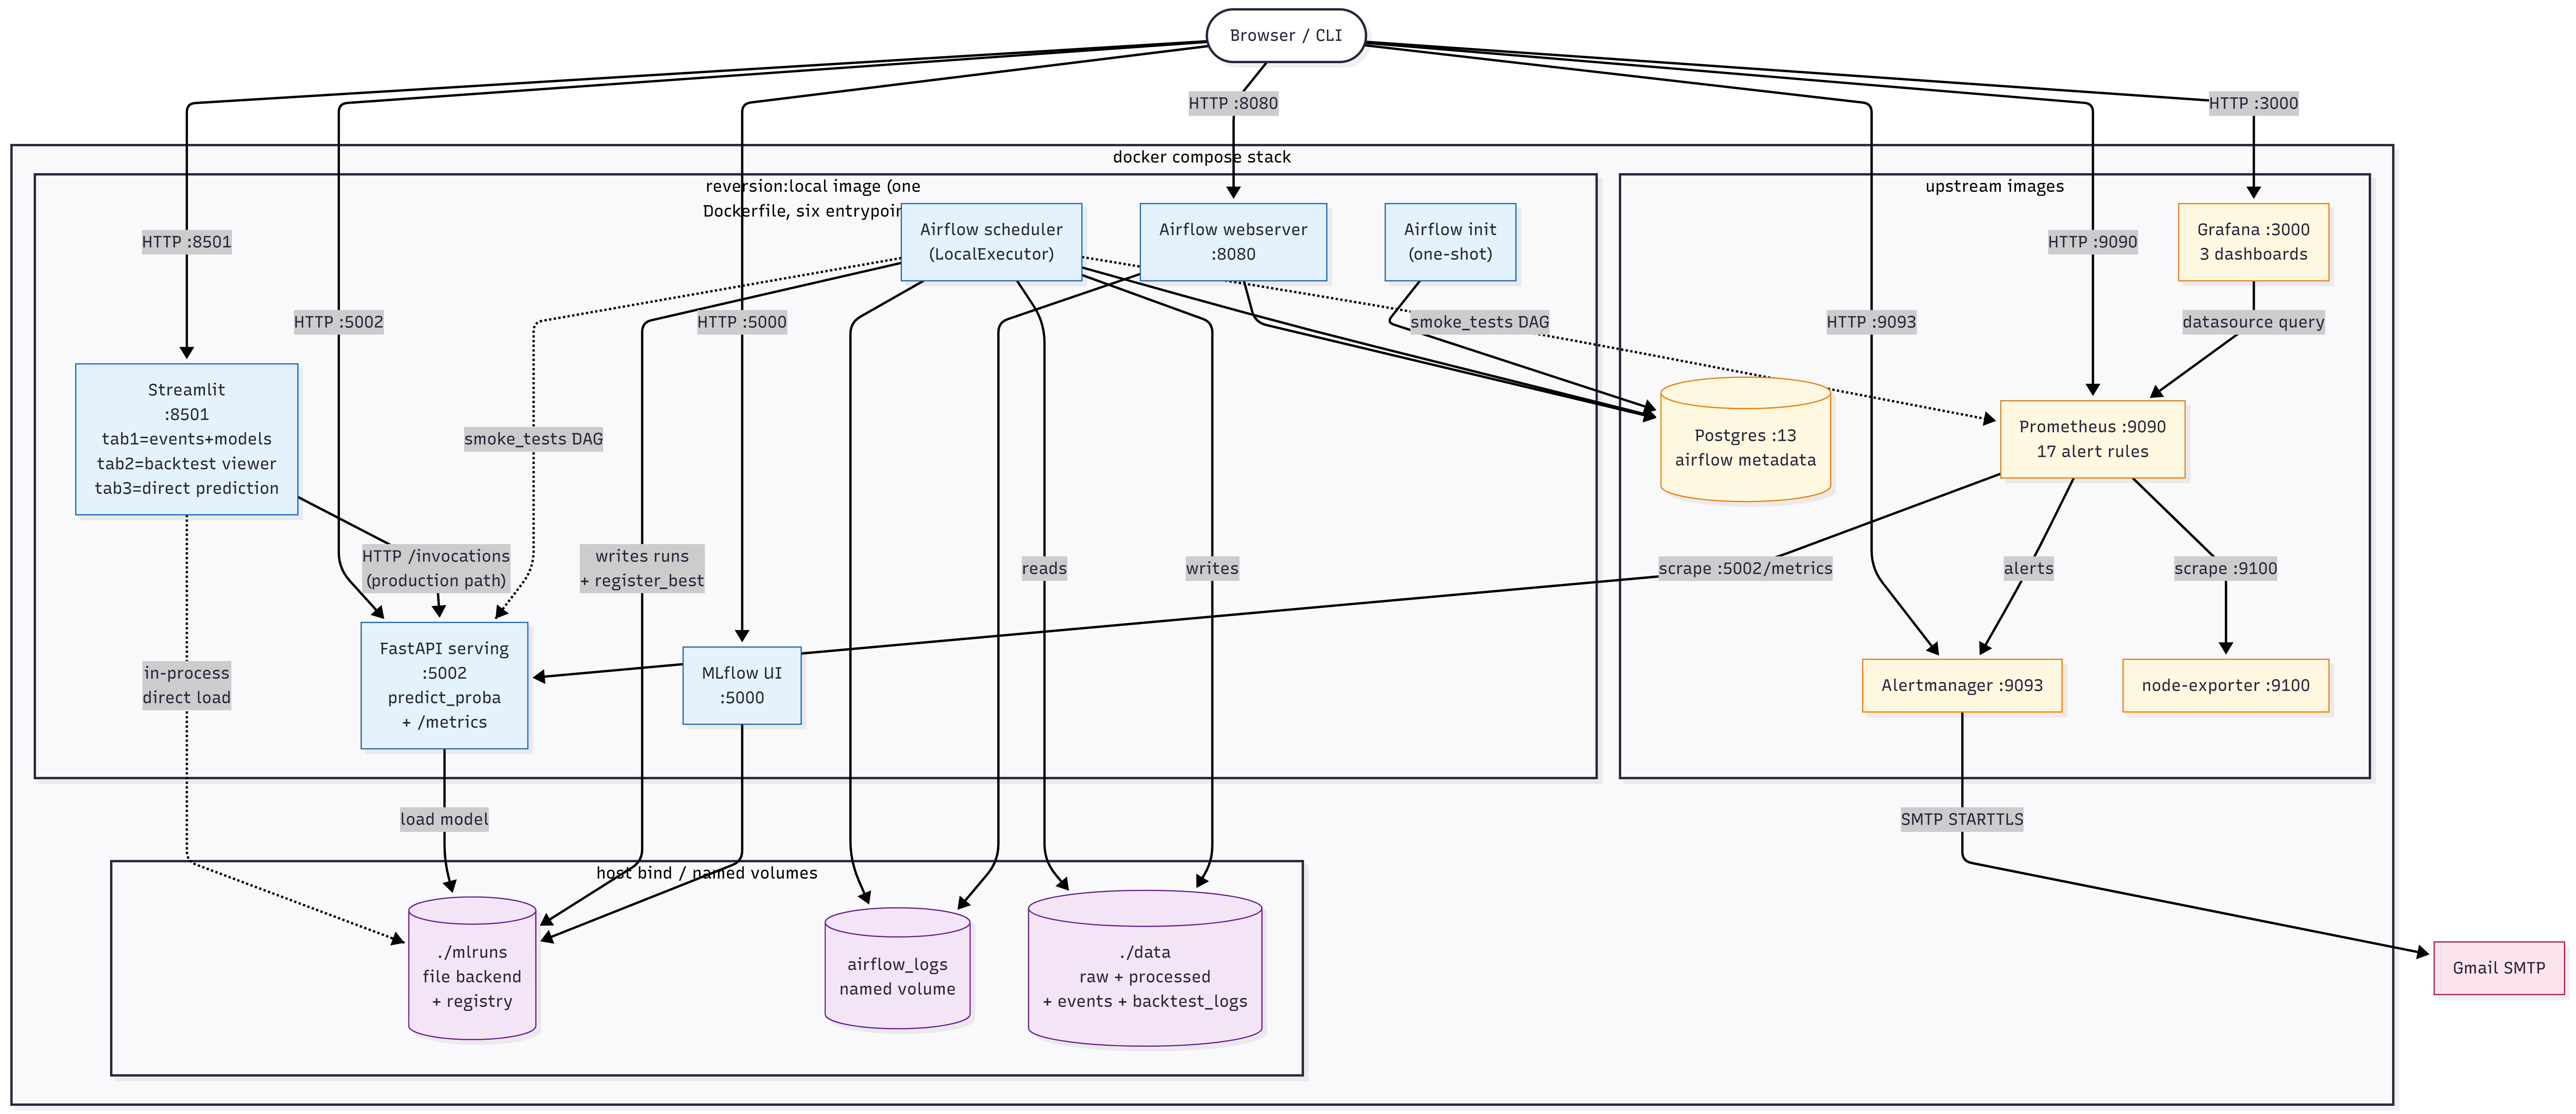
\includegraphics[width=0.9\linewidth]{images/architecture.png}
  \caption{System architecture (rendered separately).}
  \label{fig:system-architecture}
\end{figure}

\subsection{Component table}

\begin{tabularx}{\linewidth}{@{}lXl@{}}
\toprule
\textbf{Component} & \textbf{Role} & \textbf{Where} \\
\midrule
Raw data store          & Versioned source ticks (CSV + DVC, local cache only)              & \texttt{data/raw/\{2022-24,2025,dates\}.dvc} \\
Preprocess              & Per-tick merge of fut/cash/VIX, bucketing, DTE                    & \texttt{src/preprocess.py} \\
Event detection         & Outlier classification on basis spread (z-score)                  & \texttt{src/events.py} \\
Training                & RF / XGB heads $\times$ 3 positions $\times$ N symbols; logged to MLflow    & \texttt{src/mlflow\_train.py}, \texttt{src/mlflow\_grid.py} \\
Backtest                & Per-trade PnL with fixed lot size and txn cost                    & \texttt{src/backtest.py} \\
Serving                 & FastAPI wrapper around \texttt{mlflow.pyfunc}, port 5002          & \texttt{src/serve.py} \\
UI                      & Streamlit (Events / Backtest / Direct prediction tabs)            & \texttt{src/streamlit\_app.py} \\
Metrics                 & Counters, histograms, gauges, summaries                           & \texttt{src/serve\_metrics.py} \\
Alert rules             & 17 rules across serving / system / infra                          & \texttt{monitoring/alerts/} \\
Email routing           & Severity-based receivers, inhibits                                & \texttt{monitoring/alertmanager.template.yml} \\
Dashboards              & overview, model\_serving, system\_metrics                         & \texttt{monitoring/grafana/dashboards/} \\
Orchestration           & Three Airflow DAGs (pipeline, manual train, smoke)                & \texttt{airflow/dags/} \\
\bottomrule
\end{tabularx}

\subsection{Deployment topology}

\begin{tabularx}{\linewidth}{@{}lllX@{}}
\toprule
\textbf{Service} & \textbf{Image} & \textbf{Port} & \textbf{Notes} \\
\midrule
\texttt{streamlit}            & \texttt{reversion:local}     & 8501       & UI; mounts \texttt{src/}, \texttt{scripts/}, \texttt{mlruns/} \\
\texttt{mlflow-ui}            & \texttt{reversion:local}     & 5000       & file backend at \texttt{/app/mlruns} \\
\texttt{serving}              & \texttt{reversion:local}     & 5002       & \texttt{working\_dir: /app}; reads \texttt{MODEL\_URI} from \texttt{.env} \\
\texttt{airflow-init}         & \texttt{reversion:local}     & ---        & one-shot DB migrate, admin user, pool, smtp\_default \\
\texttt{airflow-webserver}    & \texttt{reversion:local}     & 8080       & DAG triggers, params, logs \\
\texttt{airflow-scheduler}    & \texttt{reversion:local}     & ---        & LocalExecutor; tasks run as scheduler subprocesses \\
\texttt{postgres}             & \texttt{postgres:13}         & ---        & Airflow metadata DB \\
\texttt{prometheus}           & \texttt{prom/prometheus}     & 9090       & scrapes \texttt{serving:5002/metrics} \\
\texttt{alertmanager}         & \texttt{prom/alertmanager}   & 9093       & rendered config from template + .env \\
\texttt{grafana}              & \texttt{grafana/grafana}     & 3000       & dashboards + datasources provisioned \\
\texttt{node-exporter}        & \texttt{prom/node-exporter}  & 9100       & host-VM metrics \\
\bottomrule
\end{tabularx}

\subsection{Architectural rationale}

\subsubsection{Loose frontend--backend coupling via REST}
The rubric requires that the inference engine and UI ``be independent software blocks connected only via (configurable) REST API calls.'' The \texttt{serving} container (FastAPI on port 5002) is the only path used by external clients --- \texttt{scripts/smoke.py} and direct \texttt{curl} both POST \texttt{dataframe\_split} payloads to \texttt{/invocations}. Streamlit's \emph{Direct prediction} tab (tab 3) deliberately bypasses this HTTP path and loads the model in-process --- see Section~\ref{sec:archdec} (\emph{Streamlit's prediction tab bypasses the FastAPI server}) for why. Even the registry-management surface is REST-shaped: ``Pin this version'' in tab~1's \emph{Registered models} expander shells out to \texttt{scripts/swap\_model.py}, which edits \texttt{.env::MODEL\_URI} and force-recreates the serving container --- not the Streamlit container. So the two services keep a clean cut: FastAPI is the only thing on the production HTTP path, and Streamlit's in-process load is a parallel diagnostic surface, not a substitute.

\subsubsection{One image, many entrypoints}
Six of eleven services run \texttt{reversion:local} (Streamlit, MLflow UI, serving, three Airflow services). The Dockerfile is one \texttt{FROM apache/airflow:2.10.3} layer plus \texttt{pip install -r requirements.txt}, so the dep set is fixed across training, serving, orchestration. Three benefits:

\begin{itemize}[leftmargin=1.5em,itemsep=0pt]
  \item \textbf{Environment parity} (rubric: ``Use Docker to ensure the development, staging, and production environments are identical''): the same interpreter and same library versions execute every code path.
  \item \textbf{One build, one cache invalidation}: changes to \texttt{requirements.txt} rebuild one image, not five.
  \item \textbf{Onboarding}: a single \texttt{docker compose up -d} brings the entire stack up. No CUDA wheels, no per-service Dockerfiles to diverge.
\end{itemize}

The five remaining services (\texttt{postgres}, \texttt{prometheus}, \texttt{alertmanager}, \texttt{grafana}, \texttt{node-exporter}) stay on upstream images because they're declarative-config services with no Python code; folding them into our image would just inflate the layer count and break upstream upgrade paths.

\subsubsection{Single source of truth: \texttt{config.yaml}}
Every \texttt{src/*.py} module reads \texttt{config.yaml} via \texttt{yaml.safe\_load} at import. Paths, schemas, hyperparameters, time buckets, split ranges, the grid sweep, and the lot/cost numbers all live there. The Airflow DAG re-reads the same file at parse time to expand the grid combos:

\begin{lstlisting}[style=pystyle]
_cfg = yaml.safe_load((PROJECT_ROOT / "config.yaml").read_text())
_POSITIONS = _cfg["backtest"]["positions"]
GRID_COMBOS = _expand("rf",  _cfg["grid"]["rf"]) \
            + _expand("xgb", _cfg["grid"]["xgb"])
\end{lstlisting}

So scaling the sweep is one edit to \texttt{config.yaml} (the DAG and \texttt{mlflow\_grid.py} both pick it up; nothing else changes).

\subsubsection{Functional decomposition with a preserve-core-logic rule}
The pipeline functions in \texttt{preprocess.py}, \texttt{events.py}, \texttt{model.py}, and \texttt{backtest.py} are kept as small, pure functions with stable signatures. New tooling (MLflow, Airflow, FastAPI, Streamlit) wraps them externally rather than editing them. Concretely:

\begin{itemize}[leftmargin=1.5em,itemsep=0pt]
  \item \texttt{mlflow\_train.py} mutates the in-memory \texttt{\_cfg} dict and calls \texttt{train\_position()} verbatim.
  \item \texttt{mlflow\_grid.py} reuses \texttt{load\_events\_all}, \texttt{prepare\_events}, \texttt{split\_events}, and \texttt{\_clean}; it bypasses \texttt{train\_position} only to swap the estimator family (RF/XGB) without editing \texttt{model.py}.
  \item Airflow DAGs are thin BashOperators around the same script CLIs.
  \item Backtest's MLflow path lives in \texttt{\_load\_models\_mlflow}, not inside any pipeline function.
\end{itemize}

This boundary is what makes new MLOps surface area additive: each new tool lands as a wrapper, not a rewrite.

\subsubsection{Why MLflow Registry, not pickles}
Backtest, Streamlit, and FastAPI all resolve models through the registry: \texttt{models:/<name>/<stage>}, \texttt{models:/<name>/<version>}, or \texttt{auto:<name>}. A pickle on disk would couple the binary to a single sklearn version and a single Python build; the registry abstracts this. \texttt{src/serve.py::\_resolve\_model\_uri} translates \texttt{auto:} on container start, so registry promotions take effect on next \texttt{docker compose up -d --force-recreate serving} --- reproducible, and inspectable in \texttt{.env}.

\subsubsection{Reproducibility ledger}
The rubric requires that ``every experiment must be reproducible via a specific Git commit hash and a corresponding MLflow run ID.'' The serving layer surfaces both as a Prometheus gauge with provenance labels:

\begin{lstlisting}[style=pystyle]
MODEL_INFO.labels(
    model_uri=MODEL_URI,
    git_commit=_git_commit(),
    mlflow_run_id=_mlflow_run_id_from_uri(MODEL_URI),
).set(1)
\end{lstlisting}

Combined with MLflow's autolog of params and the registry's run lineage, any in-production prediction can be traced to (run, commit) in two clicks: the Grafana \texttt{Model Serving} dashboard pins the labels, the registry links the run, and the run links the source commit.

\subsection{Boundaries between concerns}

\begin{itemize}[leftmargin=1.5em,itemsep=0pt]
  \item \textbf{\texttt{config.yaml} is the single source of truth} for paths, schemas, hyper-parameters, time-bucket boundaries, and split ranges. Every \texttt{src/*.py} reads it via \texttt{yaml.safe\_load}.
  \item \textbf{Airflow owns the runtime DAG.} \texttt{dvc.yaml} remains as a parallel description for ad-hoc local re-runs.
  \item \textbf{MLflow owns model versioning.} Pickles under \texttt{models/} are deprecated.
  \item \textbf{Prometheus + Grafana + Alertmanager} form an isolated observability plane; application code never reads from them.
  \item \textbf{Hidden test holdout.} \texttt{data/raw/2025/} is gated by \texttt{--split hidden --confirm-holdout}; no routine script reads from it.
\end{itemize}

\subsection{Key architecture decisions}\label{sec:archdec}

This subsection records the non-obvious design choices and their rationale. Each one was either made deliberately or learned from a concrete failure (cross-referenced to \texttt{report/ISSUES.md} where applicable).

\paragraph{Single image, multiple containers.}
One \texttt{Dockerfile} produces \texttt{reversion:local}; six app services (\texttt{streamlit}, \texttt{mlflow-ui}, \texttt{serving}, three airflow services) run that image with different entrypoints. Alternatives considered: one image per service, or one container running everything via \texttt{supervisord}. Rejected both --- per-service images explode the build matrix; supervisor hides Airflow's process model and breaks per-service health checks. Five upstream images (\texttt{postgres}, \texttt{prom/prometheus}, \texttt{prom/alertmanager}, \texttt{grafana/grafana}, \texttt{prom/node-exporter}) stay unmodified because each ships pre-configured for its role.

\paragraph{LocalExecutor, not Celery.}
Pipeline tasks run as scheduler subprocesses rather than as Celery workers. Avoids two extra services (\texttt{redis}, \texttt{airflow-worker}) and the broker handshake. Concurrency is capped by the \texttt{grid\_search} pool (cap 2) instead of worker count. Trade-off: a heavyweight scheduler crash takes the whole stack with it, but for a single-host research pipeline that risk is acceptable.

\paragraph{Idempotent preprocess via \texttt{ShortCircuitOperator}, not by editing \texttt{src/preprocess.py}.}
The user requirement was ``run preprocess only when processed data is missing.'' The natural fix --- adding an existence check inside \texttt{preprocess.py} --- would have changed function bodies, violating the project's preserve-core-logic rule. Instead, a \texttt{check\_data} ShortCircuitOperator in the DAG returns \texttt{False} when both \texttt{data/processed/} and \texttt{data/events/} are populated, skipping \texttt{preprocess} and \texttt{events}. \texttt{ignore\_downstream\_trigger\_rules=False} confines the skip to the immediate downstream; \texttt{grid\_search} declares \texttt{trigger\_rule="none\_failed"} so it runs regardless of whether the upstream stages ran or were skipped.

\paragraph{Dual \texttt{mlruns} mount path on every consumer.}
The Airflow scheduler writes MLflow runs from cwd \texttt{/opt/airflow/project}, so the file backend bakes that absolute path into each run's \texttt{meta.yaml::artifact\_uri}. The \texttt{serving}, \texttt{mlflow-ui}, and \texttt{streamlit} containers each bind-mount the host \texttt{./mlruns} at BOTH \texttt{/app/mlruns} and \texttt{/opt/airflow/project/mlruns}. Same bytes, both paths exist, so registry lookups resolve regardless of which container wrote the run. Alternative considered: HTTP-backed MLflow tracking server (eliminates absolute paths). Deferred --- adds a service, requires SQL backend migration, and the dual-mount is one yaml line per container. (See I-44.)

\paragraph{File backend for MLflow, not a tracking server.}
\\
\texttt{mlflow ui --backend-store-uri=file:/app/mlruns}. Pros: zero extra infra, no DB to migrate, runs and registry on the same volume. Cons: the absolute-path issue (handled by the dual mount), no concurrent writers across processes (not an issue with grid pool cap 2 and per-task subprocesses). For a research-scale pipeline this beats a tracking server.

\paragraph{XGB output wrapped to return string labels.}
XGBoost requires numeric class targets, so \texttt{mlflow\_grid.py} LabelEncodes \texttt{klass} before fit. The naive \texttt{mlflow.sklearn.log\_model(xgb\_clf)} loses the encoder, so consumers that load the registered XGB and call \texttt{predict()} get ints back --- which then collide with the string \texttt{klass} column in \texttt{backtest.evaluate} (\texttt{ValueError: Mix of label input types}). The \texttt{XGBStringClassifier} wrapper pairs the fitted XGB with its LabelEncoder and inverse-transforms inside \texttt{predict}. RF is unaffected and logs unwrapped. (See I-47.)

\paragraph{\texttt{n\_jobs=1} for grid estimators.}
With pool cap 2, two grid tasks run concurrently. \texttt{n\_jobs=-1} on each makes both grab all cores, which thrashes the Linux scheduler and stalls tasks indefinitely. Setting \texttt{n\_jobs=1} keeps each task on one core; two run cleanly in parallel and total wall-time on the smallest grid drops from ``indefinite'' to ${\sim}3$ minutes. (See I-48.)

\paragraph{Smoke tests as a separate DAG, not a final stage.}
\texttt{smoke\_tests} runs every 30 min independent of pipeline triggers. Folding the smoke checks into \texttt{reversion\_pipeline}'s tail would only exercise them on the weekly trigger; failures between trainings would go undetected until the next run. Independent scheduling catches drift (model server crashed, Prometheus target down) within 30 minutes regardless of pipeline activity.

\paragraph{One swap backend, two front-ends.}
\texttt{scripts/swap\_model.py} owns the logic: validate \texttt{(name, version)} via MLflow client, rewrite the \texttt{MODEL\_URI=} line in \texttt{.env}, force-recreate the \texttt{serving} container. The Streamlit \emph{Registered models} expander (top of tab 1) imports nothing from the script --- it shells out to it via \texttt{subprocess.run}. Single source of truth for the swap operation; the UI is a thin trigger.

\paragraph{\texttt{config.yaml::grid} as the single source for the sweep.}
The Airflow DAG (dynamic task mapping) and the CLI (\texttt{mlflow\_grid.py}) both compute their combos from \texttt{config.yaml::grid}. Editing those lists scales both runners simultaneously. Avoids the previous failure mode where a bash wrapper and the DAG defined the grid independently and silently diverged.

\paragraph{Defensive failure modes for SMTP and the EmailOperator.}
\texttt{notify\_complete} declares \texttt{trigger\_rule="all\_done"} so a mis-configured SMTP doesn't poison the dagrun.
\\
The \texttt{smtp\_default} connection's extras must use the modern key names (\texttt{disable\_ssl}/\texttt{disable\_tls}); legacy \texttt{smtp\_starttls}/\texttt{smtp\_ssl} are silently ignored, leaving both \texttt{disable\_*} at \texttt{false} default which forces implicit SSL on port 587 and breaks Gmail STARTTLS. (See I-51.)

\paragraph{Streamlit's prediction tab bypasses the FastAPI server.}
The serving container loads exactly one head per process --- \texttt{MODEL\_URI} resolves to a single registered model at startup. Switching between classifier, duration, and revert heads at the same (symbol, position) in an interactive UI would require bouncing the container per click, which is not interactive. \texttt{streamlit\_app.py} therefore loads the requested head directly via \texttt{mlflow.sklearn.load\_model(...)} in the Streamlit process and calls \texttt{.predict()} synchronously. Trade-off: this path generates no Prometheus traffic and so does not populate the \texttt{prediction\_score} histogram --- the production HTTP path (\texttt{scripts/smoke.py predict}, real clients) remains the canonical source of serving metrics. Up to $3 \times 3 \times |\text{symbols}|$ model objects (one per head--position--symbol) live in the Streamlit process via \texttt{@st.cache\_resource}; with the current 2-symbol setup that's 18 cached estimators at most.

\paragraph{Direct load uses \texttt{runs:/} URIs,
not \texttt{models:/}.}
\\

\texttt{mlflow.sklearn.load\_model("models:/<name>/<version>")} writes a \texttt{registered\_model\_meta} sidecar file next to the source artefact to record provenance. This fails with \texttt{OSError [Errno 30] read-only file system} when the calling container has \texttt{mlruns/} mounted RO (the airflow scheduler does, at \texttt{/opt/airflow/project/mlruns}). The Streamlit loader resolves the version through \texttt{MlflowClient.get\_latest\_versions(...)} and then loads via \texttt{runs:/<run\_id>/model\_<head>}, which goes directly to the run's artefact directory and skips the sidecar write. Same model bytes, no provenance side-effect, works regardless of mount mode.

\paragraph{Per-symbol models, not pooled.}
The model trains per (\emph{symbol}, \emph{position}) rather than pooling across symbols. BAJFINANCE and RELIANCE have different microstructure --- lot multiplier, OI scale, bid-ask geometry, scheduled-event cadence --- and even after symbol-conditional z-score normalisation those structural differences leak through features like \texttt{det\_oi\_fut}, \texttt{det\_ltq}, and the bid-ask widths.
\\

A single model trained on the union confuses the regimes. We considered pooling for training-data efficiency and rejected it on the same grounds the conditional distribution argument applies to: a $2\sigma$ event for one symbol is not the same kind of event for the other. Concretely: \texttt{src/mlflow\_grid.py} now requires \texttt{--symbol}, filters \texttt{(position, symbol)} before fitting, and tags the run; \texttt{scripts/register\_best.py} sweeps \texttt{(position $\times$ symbol)} and registers under
\\
\texttt{reversion-\{head\}-pos\{p\}-\{symbol\}}. 
\\
The Airflow grid mapping doubles to $|\text{symbols}| \times |\text{positions}| \times |\text{hyperparams}|$ combos. Cost: 2$\times$ the training tasks; benefit: no symbol-blind regime smearing, and clean per-symbol drift signals downstream. Adding a third ticker means adding it to \texttt{config.yaml::symbols} and re-running the DAG --- no model changes needed.

\paragraph{Sample predictions logged via \texttt{log\_text}/\texttt{log\_dict}, not temp files.}
\texttt{mlflow\_grid.py} and \texttt{mlflow\_train.py} previously wrote a temp CSV to \texttt{ROOT/} before calling \texttt{mlflow.log\_artifact(...)}. \texttt{ROOT} resolves to \texttt{/opt/airflow/project/} in the airflow scheduler, where bind-mounted \texttt{src/}, \texttt{scripts/}, and \texttt{config.yaml} make the parent directory effectively read-only - the temp write throws \texttt{Errno 13}. 
\\
The fix is to skip disk entirely: 
\\
\texttt{mlflow.log\_text(buf.getvalue(), "predictions/sample\_predictions.csv")} for the CSV and \texttt{mlflow.log\_dict(synth\_doc, "predictions/synthetic\_example.json")} for the synthetic example. Both write directly into the run's artefact store under MLflow's tracking root (which IS writable --- it's the dual-mounted \texttt{mlruns/}). 
\\
Side benefit: the static \texttt{metrics/sample\_prediction.\{csv,json\}} files are no longer needed; every grid run now ships its own samples paired to the (symbol, position, hp) that produced them.

% =========================================================================
\section{Functional Decomposition}
% =========================================================================

\subsection{Data ingestion and preprocessing --- \texttt{src/preprocess.py}}
Reads raw CSVs from \texttt{data/raw/\{2022-24,2025\}/\{symbol\}/\{contract\}/\{day\}.csv}; merges futures, equity, and VIX feeds tick-aligned via \texttt{pandas.merge\_asof}; filters by VIX threshold
\\
(\texttt{config.yaml::preprocess.vix\_thresh}); stratifies output by \texttt{(symbol, dte\_bucket, time\_bucket)} so the event detector can compute per-bucket distributions. Writes \texttt{data/processed/\{symbol\}\_\{dte\}\_\{bucket\}.csv}.

\subsection{Event detection --- \texttt{src/events.py}}
For each \texttt{(symbol, dte, bucket)} group, computes a rolling z-score of the basis spread; flags ticks where $|z|$ exceeds \texttt{out\_thresh} as \emph{detection} events; walks forward to find resolution: first tick where $|z|<$ \texttt{rev\_thresh} (reversion) OR $|z|>k\cdot$ \texttt{out\_thresh} (divergence); EOD without trigger gives continuation. Writes \texttt{data/events/\{symbol\}.csv}.

\subsection{Training --- \texttt{src/mlflow\_train.py}, \texttt{src/mlflow\_grid.py}}
Loads events, splits by date range (\texttt{train\_range} / \texttt{val\_range} / \texttt{dev\_test\_range} / \texttt{hidden\_range}). Per (\emph{symbol}, \emph{contract position}) pair --- positions $\in\{0,1,2\}$, symbols from \texttt{config.yaml::symbols} --- trains 3 heads: classifier (\texttt{klass}), duration regressor (\texttt{duration\_sec}), revert-delta regressor (\texttt{revert\_delta}). \texttt{mlflow\_train.py} is a single-config baseline run; \texttt{mlflow\_grid.py} sweeps RF / XGB hyper-parameters and is the canonical entry point. Both require \texttt{--symbol}; pre-filtering happens externally in the caller, so \texttt{model.py::train\_position} stays untouched per the preserve-core-logic rule. Best runs are promoted to the MLflow Registry by \texttt{scripts/register\_best.py}, which sweeps (position $\times$ symbol) and registers as \texttt{reversion-\{head\}-pos\{p\}-\{symbol\}}.

\subsection{Backtest --- \texttt{src/backtest.py}}
For each event in the eval split, the classifier head emits \texttt{pred\_klass}. A trade is opened on \texttt{reversion} (bet on narrowing) and \texttt{divergence} (bet on widening, sign-flipped). \texttt{continuation} $\to$ no trade. PnL = entry cashflow + exit cashflow $-$ transaction cost. Lot size and txn-cost rate from \texttt{config.yaml::backtest}. Models are loaded per (symbol, position) via \texttt{runs:/<run\_id>/...} URIs (RO-mount safe); the eval split is filtered per symbol before \texttt{evaluate()} so each model only scores its own symbol's events. Writes \texttt{data/backtest\_logs/trades\_\{symbol\}\_position\_*\_\{val,hidden\}.csv} --- 6 files per split.

\subsection{Serving --- \texttt{src/serve.py}}
FastAPI app loading the MLflow \texttt{pyfunc} flavoured classifier head from \texttt{MODEL\_URI} 
\\
(e.g. \texttt{models:/reversion-classifier-pos0-BAJFINANCE/Production}). Endpoints:
\begin{itemize}[leftmargin=1.5em,itemsep=0pt]
  \item \texttt{POST /invocations} --- MLflow-compatible payload, returns \texttt{predictions}.
  \item \texttt{GET /health} --- always 200; cheap liveness probe.
  \item \texttt{GET /ready} --- 503 until the model is loaded \emph{and} a dummy predict succeeds.
  \item \texttt{GET /metrics} --- Prometheus exposition.
\end{itemize}
Resolves \texttt{auto:<name>} URIs to the latest Production version via the MLflow client at startup, so a fresh registry promotion reaches serving on next container restart.

\subsection{Model registry stages and promotion}

After \texttt{scripts/register\_best.py} runs, MLflow holds three registered model names per (\emph{position}, \emph{symbol}) pair (\texttt{reversion-classifier-pos$i$-$s$}, \texttt{reversion-duration-pos$i$-$s$}, \texttt{reversion-revert-pos$i$-$s$} for $i \in \{0,1,2\}$ and $s \in \texttt{symbols}$), each with an ordered list of versions. With 2 symbols configured, that's $3 \times 3 \times 2 = 18$ registered names. Every version carries a \texttt{current\_stage} field $\in$ \{\texttt{None}, \texttt{Staging}, \texttt{Production}, \texttt{Archived}\}. Newly registered versions land in \texttt{None}; \texttt{--promote} transitions them to \texttt{Production} with \texttt{archive\_existing\_versions=True} (\texttt{scripts/register\_best.py:113--117}), so the previous Production version is auto-Archived in the same call.

\textbf{What is materially different about a Production version.} Nothing about the artefact itself: the byte stream is identical to the same version in any other stage. The stage is purely a routing tag. Two consequences flow from it:

\begin{itemize}[leftmargin=1.5em,itemsep=0pt]
  \item \texttt{models:/<name>/Production} resolves to the version currently in that stage. Non-Production versions are not addressable by this URI.
  \item The \texttt{auto:<name>} resolver in \texttt{src/serve.py:39--61} prefers Production: 
  \\
  it returns \texttt{models:/<name>/Production} when one exists, else falls back to the latest version in stage \texttt{None}. So a server running with \texttt{MODEL\_URI=auto:reversion-classifier-pos0-BAJFINANCE} rolls forward to whatever was promoted most recently when next reloaded.
\end{itemize}

\textbf{What is not gated by Production.} Metrics, alerts, the Grafana dashboards, the backtest CLI, and unit tests are all stage-agnostic. There is no statistical guard between the previous and the new Production version. \texttt{register\_best.py --promote} performs an unconditional cutover: the run with the highest \texttt{f1\_macro} per position wins, and all three heads from that run are promoted together --- regressor MAEs do not enter the selection.

\subsection{UI --- \texttt{src/streamlit\_app.py}}
Three tabs. Tab 1 hosts a \emph{Registered models} expander at the top that lists registry contents and exposes pin / promote buttons; the buttons shell out to \texttt{scripts/swap\_model.py} or call \texttt{client.transition\_model\_version\_stage} respectively.
\begin{enumerate}[leftmargin=1.5em,itemsep=0pt]
  \item \textbf{Event explorer} --- runs \texttt{events.run()} for a chosen \texttt{(symbol, year, month, day)}.
  \item \textbf{Backtest viewer} --- loads persisted trade logs, plots equity curve.
  \item \textbf{Direct prediction} --- pick symbol $\to$ contract expiry $\to$ derive position $\to$ pick head $\to$ load via \texttt{mlflow.sklearn.load\_model("runs:/...")} and call \texttt{predict()}. Bypasses the FastAPI server (rationale in Section~\ref{sec:archdec}).
\end{enumerate}

\subsection{Observability stack}
\texttt{serve.py} exposes counters (\texttt{prediction\_requests\_total}, \texttt{prediction\_errors\_total}), histograms (\texttt{prediction\_latency\_seconds}, \texttt{prediction\_score}), gauges (\texttt{inference\_in\_flight}, \texttt{model\_memory\_bytes}, \texttt{model\_info}), and a summary (\texttt{payload\_rows}). 17 alert rules across \texttt{monitoring/alerts/} (serving / system / infra). Alertmanager routes \texttt{critical} and \texttt{warning} severities to two Gmail receivers, with \texttt{ModelServerDown} inhibiting downstream alerts. Three Grafana dashboards: \texttt{overview}, \texttt{model\_serving}, \texttt{system\_metrics}.

\subsection{Drift surfaces}

Three drift signals are surfaced today, all output- or schema-side; no input-feature drift is computed in the current build.

\begin{itemize}[leftmargin=1.5em,itemsep=0pt]
  \item \textbf{Prediction-score distribution} --- the \texttt{prediction\_score} histogram (\texttt{src/serve\_metrics.py:32--37}) records every numeric prediction served. It is the foundation for prediction drift: a quantile shift on this histogram week-over-week is the fastest signal that the served model has started behaving differently. The histogram is populated and retained by Prometheus; no alert rule consumes it today.
  \item \textbf{Schema-drift proxy via 4xx} --- the \texttt{High4xxRate} alert (\texttt{monitoring/alerts/serving.yml}) fires when the 4xx ratio exceeds 20\% for 5 minutes. The annotation explicitly tags this as ``payload schema drift?''. It is a downstream proxy: it catches clients sending wrong-shape payloads, not feature distribution shift in the rows themselves.
  \item \textbf{Latency regression vs.\ baseline} --- \texttt{ModelLatencyDegraded} compares the 5m p95 to the 1h p95 from one hour ago and fires on a $2\times$ excess. This catches the model becoming slower (e.g.\ after a hot-swap to a heavier estimator), not its outputs changing.
\end{itemize}

\textbf{Gaps.} There is no PSI / KS / Wasserstein on input features, no Evidently or whylogs job exporting per-feature distribution stats, no champion-vs-challenger shadow scoring during promotion, and no quantile alert on the \texttt{prediction\_score} histogram. The hooks are in place; only the comparators and rules are missing.

\textbf{Planned input-feature drift detection.} The rubric requires monitoring of input distribution shift; the design below closes this gap and is the next slice of MLOps surface area to land. It reuses the per-shard expanding statistics already produced by \texttt{src/preprocess.py} (no recomputation), so drift evaluation is cheap.

\begin{enumerate}[leftmargin=1.5em,itemsep=0pt]
  \item \textbf{Frozen baseline at training cut-off.} On every \texttt{register\_best.py --promote}, snapshot the per-feature distribution over \texttt{model.train\_range} into \texttt{data/baselines/feature\_baseline\_<train\_end>.json}. Format:
\begin{lstlisting}[style=bashstyle]
{
  "train_end": "2024-05",
  "symbol":    "BAJFINANCE",
  "position":  0,
  "n_rows":    18420,
  "features": {
    "det_z_score":  {"mean": 0.02, "std": 1.01,
                     "quantiles": {"p01": -2.4, "p10": -1.3, "p50": 0.01,
                                   "p90": 1.32, "p99": 2.45},
                     "bins": [<10 edges>], "hist": [<9 counts>]},
    "det_spread":   {...},
    ...   /* one entry per feature in model.feature_cols */
  }
}
\end{lstlisting}
  Tracked in DVC, one file per (\emph{symbol}, \emph{position}) so per-symbol drift is computable independently. Baseline regenerates only when \texttt{train\_range} changes; routine promotions reuse the existing file.
  \item \textbf{Scheduled PSI computation.} Add an Airflow DAG \texttt{drift\_check} on a daily schedule. For each (\emph{symbol}, \emph{position}), join the served-feature stream from the last 24h (logged by \texttt{serve.py} as JSON lines under \texttt{logs/predictions/*.jsonl}) with the baseline's bin edges and compute Population Stability Index per feature: $\text{PSI} = \sum_i (a_i - b_i) \cdot \ln(a_i / b_i)$, where $a_i$ is the live histogram fraction and $b_i$ is the baseline fraction in bin $i$. Standard thresholds: $<\!0.10$ stable, $0.10\!-\!0.20$ moderate, $>\!0.20$ shifted.
  \item \textbf{Prometheus surface.} Pushgateway-exposed gauge:
\begin{lstlisting}[style=bashstyle]
feature_psi{feature="det_z_score", symbol="BAJFINANCE", position="0"} 0.084
feature_psi{feature="det_spread",  symbol="BAJFINANCE", position="0"} 0.231
\end{lstlisting}
  The \texttt{symbol} and \texttt{position} labels are required by the per-symbol model boundary --- a $0.20$ PSI on RELIANCE pos 1 must not silently average with BAJFINANCE pos 0 (per the per-symbol-model architecture decision in Section~\ref{sec:archdec}, \emph{Per-symbol models, not pooled}).
  \item \textbf{Alert rule.} \texttt{monitoring/alerts/serving.yml} adds:
\begin{lstlisting}[style=bashstyle]
- alert: FeatureDriftHigh
  expr: max by (feature, symbol, position) (feature_psi) > 0.20
  for: 1h
  labels: {severity: warning}
  annotations:
    summary: "Feature {{$labels.feature}} drift on {{$labels.symbol}} pos {{$labels.position}} (PSI={{$value}})"
\end{lstlisting}
  Routed to the warning receiver; \texttt{ModelServerDown} continues to inhibit it (no point alerting on drift if the server is gone).
  \item \textbf{Prediction-score quantile alert.} Companion rule on the existing \texttt{prediction\_score} histogram --- alert when the 7-day p95 of max-class confidence drops more than 20\% vs.\ a 30-day baseline (proxy for prediction drift).
\end{enumerate}

\textbf{Planned ground-truth feedback loop.} The rubric also requires logging of realised labels for production-decay tracking. Today, labels are only computed offline by \texttt{events.py} on the 2022--24 / 2025 splits; nothing pairs served predictions with their realised \texttt{klass}. The design:

\begin{enumerate}[leftmargin=1.5em,itemsep=0pt]
  \item \textbf{Prediction trace.} \texttt{serve.py} writes one JSON line per request to \texttt{logs/predictions/<YYYY-MM-DD>.jsonl}, with fields \texttt{event\_id} (UUID4), \texttt{det\_timestamp}, \texttt{symbol}, \texttt{contract}, \texttt{features}, \texttt{pred\_klass}, \texttt{model\_uri}, \texttt{git\_commit}, \texttt{mlflow\_run\_id}. The same file is what the drift job reads in step 2 above.
  \item \textbf{Nightly join DAG.} New Airflow DAG \texttt{ground\_truth\_join} runs at \texttt{30 19 * * 1-5} (after EOD). Steps: read the previous trading day's \texttt{logs/predictions/*.jsonl}; run \texttt{events.py} on that day's raw ticks (this gives the realised \texttt{klass}); join on \texttt{(symbol, contract, det\_timestamp)} with a $\pm$1 tick tolerance; write \texttt{data/feedback/<YYYY-MM-DD>.csv} with columns \texttt{[event\_id, pred\_klass, klass, model\_uri, git\_commit]}.
  \item \textbf{Production F1 metric.} A small Python step in the same DAG computes rolling 7-day and 30-day \texttt{f1\_macro} per (\emph{model\_uri}) and pushes them to Pushgateway as \texttt{production\_f1\{window="7d", model\_uri="..."\}}. The Grafana \texttt{Model Serving} dashboard adds a panel that overlays val-F1 (from MLflow) against rolling production F1; a sustained gap is the canonical decay signal.
  \item \textbf{Decay alert.} \texttt{ProductionF1Decay} fires when \texttt{(val\_f1 - production\_f1\_30d) / val\_f1 > 0.20} for 24h, routed to the warning receiver. This complements the input-feature PSI alert (drift in inputs) with a realised-output alert (drift in model behaviour).
\end{enumerate}

The two loops together --- input-distribution PSI plus ground-truth label decay --- close the rubric's drift requirement and give the operator two independent signals before a Production model needs to be re-trained or rolled back.

\subsection{Data contracts}

\begin{tabularx}{\linewidth}{@{}llXX@{}}
\toprule
\textbf{Boundary} & \textbf{Producer} & \textbf{Consumer} & \textbf{Schema} \\
\midrule
Raw $\to$ Processed         & \texttt{preprocess.py}                 & \texttt{events.py}                       & det\_* cols + bucket / dte / VIX-filtered ticks \\
Processed $\to$ Events      & \texttt{events.py}                     & \texttt{model.py}, \texttt{backtest.py}  & det/ext/res snapshots + \texttt{klass} label \\
Events $\to$ MLflow         & \texttt{mlflow\_grid.py}               & MLflow store                             & \texttt{feature\_cols} (12) + 3 targets \\
MLflow $\to$ Serving        & Registry                               & \texttt{serve.py}                        & \texttt{mlflow.pyfunc} \\
Serving $\to$ Prometheus    & \texttt{/metrics}                      & Prometheus                               & OpenMetrics \\
Prometheus $\to$ Alertmgr   & rules eval                             & Alertmanager                             & alert objects \\
\bottomrule
\end{tabularx}

\subsection{Security posture}\label{sec:security}
Trading data and SMTP credentials are sensitive. The current build runs on a single host and is intentionally not internet-facing; the security posture below documents the boundary that already exists and what would change for a production deployment.

\begin{itemize}[leftmargin=1.5em,itemsep=0pt]
  \item \textbf{Secrets at rest.} \texttt{.env} carries \texttt{SMTP\_USER}, \texttt{SMTP\_APP\_PASSWORD}, and \texttt{ALERT\_TO}; it is \texttt{.gitignored} and rendered into Alertmanager config at container start (\texttt{monitoring/alertmanager.template.yml}). No credentials are baked into images. Disk-level encryption on the host is assumed but not enforced by the stack.
  \item \textbf{Secrets in transit.} Internal traffic between the eleven containers is plain HTTP on the user-defined Docker bridge network. SMTP to Gmail uses STARTTLS on port 587 (Airflow \texttt{smtp\_default} connection extras: \texttt{disable\_ssl=true}, \texttt{disable\_tls=false}; see I-51).
  \item \textbf{External exposure.} Only \texttt{localhost} ports are published; nothing is reachable from outside the host. There is no auth on the Streamlit, MLflow, or FastAPI surfaces --- they sit behind the host firewall.
  \item \textbf{Hidden holdout.} \texttt{data/raw/2025/} is gated by \texttt{--split hidden --confirm-holdout} on \texttt{backtest.py} and is excluded from Streamlit and the smoke load generator (project rule, enforced at the script boundary).
  \item \textbf{Production deltas (not implemented; documented for completeness).} TLS termination at a reverse proxy in front of FastAPI; basic-auth or OAuth on the Airflow / MLflow / Grafana / Streamlit UIs; secrets in a dedicated vault rather than \texttt{.env}; and audit logging on the swap-model path.
\end{itemize}

\subsection{Resource posture and model footprint}\label{sec:resource}
The rubric flags ``no cloud'' as a constraint and lists quantization / pruning as optimization options. The two registered estimator families fit comfortably below host limits without compression, so neither is applied:

\begin{tabularx}{\linewidth}{@{}lXl@{}}
\toprule
\textbf{Resource} & \textbf{Source} & \textbf{Observed} \\
\midrule
RF model artefact size      & \texttt{mlruns/<run>/artifacts/model\_classifier/}                       & 2--6 MB per head \\
XGB model artefact size     & same                                                                     & 1--3 MB per head \\
Serving RSS                 & \texttt{model\_memory\_bytes} gauge / \texttt{docker stats serving}       & $<$ 500 MB steady \\
Serving CPU (idle)          & \texttt{docker stats serving}                                            & $<$ 5\% \\
Single-host deployment      & 11 containers, 1 user image, 5 upstream                                  & runs on a 16 GB / 4-core dev box \\
\bottomrule
\end{tabularx}

Quantization and pruning are deferred: RF/XGB are already lightweight, the model fits in CPU L2/L3 cache, and \texttt{predict()} latency is dominated by FastAPI request overhead, not by the matrix multiply. If the deployment moves to per-symbol $\times$ per-position serving (one container per pair, 18 containers), memory budget per process becomes the binding constraint and a quantization pass would be revisited.

\newpage
% =========================================================================
\section{Low-Level Design --- API and CLI Specifications}\label{sec:lld}
% =========================================================================

This section is the formal LLD: each externally-callable surface is enumerated with HTTP method (or CLI signature), path, request schema, response schema per status code, error envelope, and a worked example. Three surfaces are covered: the FastAPI serving endpoints, the \texttt{swap\_model.py} CLI, and the Streamlit-to-MLflow internal contract.

\subsection{FastAPI serving --- endpoint catalogue}

Base URL inside the Compose network: \texttt{http://serving:5002}. From the host: \texttt{http://localhost:5002}. All endpoints are unauthenticated (single-host deployment, see \S~\ref{sec:security}). The implementation is in \texttt{src/serve.py}; metrics declarations are in \texttt{src/serve\_metrics.py}.

\begin{tabularx}{\linewidth}{@{}lllX@{}}
\toprule
\textbf{Method} & \textbf{Path} & \textbf{Purpose} & \textbf{Status codes} \\
\midrule
POST & \texttt{/invocations} & Score one or more feature rows                  & 200, 400, 422, 500, 503 \\
GET  & \texttt{/health}      & Liveness probe (cheap, always 200 once up)      & 200 \\
GET  & \texttt{/ready}       & Readiness probe (real predict on synthetic row) & 200, 503 \\
GET  & \texttt{/metrics}     & Prometheus exposition                            & 200 \\
\bottomrule
\end{tabularx}

\subsubsection{POST /invocations}

\textbf{Purpose.} MLflow-compatible scoring endpoint. Wraps the \texttt{pyfunc} flavoured classifier head loaded from \texttt{MODEL\_URI}.

\textbf{Request headers.} \texttt{Content-Type: application/json} (required).

\textbf{Request body schema} (\texttt{dataframe\_split} envelope):
\begin{lstlisting}[style=bashstyle]
{
  "dataframe_split": {
    "columns": [<string>, ...],   # must be a permutation of feature_cols (12)
    "data":    [[<number>, ...], ...]   # one row per prediction; len(row) == len(columns)
  }
}
\end{lstlisting}

\textbf{Field constraints.}
\begin{itemize}[leftmargin=1.5em,itemsep=0pt]
  \item \texttt{columns} must contain exactly the 12 names in \texttt{config.yaml::model.feature\_cols}: \texttt{det\_z\_score, det\_spread, side, dte, bucket, det\_dist\_std, det\_dist\_count, det\_fut\_ltq, det\_oi\_fut, det\_ltq, det\_fut\_ba, det\_eq\_ba}. Order is free; missing or extra columns return \texttt{422}.
  \item \texttt{data} rows must be numeric (\texttt{int} or \texttt{float}); \texttt{null} or strings return \texttt{422}.
  \item Empty \texttt{data} array (zero rows) returns \texttt{400}.
  \item Maximum payload size is 1 MB (FastAPI default; not yet tuned).
\end{itemize}

\textbf{Response 200 schema}:
\begin{lstlisting}[style=bashstyle]
{
  "predictions": [<string>, ...]   # one label per input row; values in {reversion, divergence, continuation}
}
\end{lstlisting}

\textbf{Response 400 / 422 / 500 / 503 schema} (error envelope):
\begin{lstlisting}[style=bashstyle]
{
  "detail": <string>   # human-readable error message
}
\end{lstlisting}

\textbf{Status code semantics.}
\begin{itemize}[leftmargin=1.5em,itemsep=0pt]
  \item \texttt{200} --- prediction succeeded; \texttt{predictions} length equals \texttt{data} length.
  \item \texttt{400} --- malformed envelope (missing \texttt{dataframe\_split}, empty \texttt{data}).
  \item \texttt{422} --- schema violation (wrong column set, non-numeric cell, FastAPI/Pydantic validation).
  \item \texttt{500} --- model raised inside \texttt{predict()}; counted in \texttt{prediction\_errors\_total\{kind="exception"\}}.
  \item \texttt{503} --- model not loaded yet (startup race; same condition that makes \texttt{/ready} return 503).
\end{itemize}

\textbf{Worked example.}
\begin{lstlisting}[style=bashstyle]
# Request
POST /invocations HTTP/1.1
Content-Type: application/json

{
  "dataframe_split": {
    "columns": ["det_z_score","det_spread","side","dte","bucket",
                "det_dist_std","det_dist_count","det_fut_ltq","det_oi_fut",
                "det_ltq","det_fut_ba","det_eq_ba"],
    "data": [[2.41, 0.087, 1, 5, 3, 0.041, 1820, 12, 4500, 8, 0.05, 0.04]]
  }
}

# Response
HTTP/1.1 200 OK
Content-Type: application/json

{"predictions": ["reversion"]}
\end{lstlisting}

\textbf{Side effects.} Increments \texttt{prediction\_requests\_total\{code="200"\}}, observes \texttt{prediction\_latency\_seconds}, increments \texttt{inference\_in\_flight} for the duration of the call, and observes \texttt{payload\_rows} once per call. On 5xx, also increments \texttt{prediction\_errors\_total}.

\subsubsection{GET /health}

\textbf{Purpose.} Liveness probe. Returns \texttt{200} as soon as the process is accepting connections; does not exercise the model.

\textbf{Request.} No body.

\textbf{Response 200 schema}:
\begin{lstlisting}[style=bashstyle]
{
  "status": "ok",
  "model_uri": <string>     # the resolved MODEL_URI (after auto: resolution)
}
\end{lstlisting}

\textbf{Worked example.} \texttt{curl http://serving:5002/health} $\to$ \texttt{200 \{"status":"ok","model\_uri":"models:/reversion-classifier-pos0-BAJFINANCE/Production"\}}.

\subsubsection{GET /ready}

\textbf{Purpose.} Readiness probe. Returns \texttt{200} only when the model is loaded \emph{and} a predict on a synthetic row succeeds.

\textbf{Synthetic payload}. The probe builds a 1-row dataframe with the 12 \texttt{feature\_cols} populated as follows (see \texttt{src/serve.py}): \texttt{det\_z\_score=2.0}, \texttt{det\_spread=0.05}, \texttt{side=1}, \texttt{dte=5}, \texttt{bucket=3}, \texttt{det\_dist\_std=0.04}, \texttt{det\_dist\_count=1000}, \texttt{det\_fut\_ltq=10}, \texttt{det\_oi\_fut=5000}, \texttt{det\_ltq=8}, \texttt{det\_fut\_ba=0.05}, \texttt{det\_eq\_ba=0.04}. The values are deliberately mid-distribution so the probe is exercised but never raises a class-imbalance edge case.

\textbf{Response 200 schema}:
\begin{lstlisting}[style=bashstyle]
{"status": "ready"}
\end{lstlisting}

\textbf{Response 503 schema}:
\begin{lstlisting}[style=bashstyle]
{"detail": <string>}    # e.g. "model not loaded yet" or "predict failed: <repr(exc)>"
\end{lstlisting}

\textbf{Worked example.} \texttt{curl -i http://serving:5002/ready} during boot returns \texttt{503 \{"detail":"model not loaded yet"\}}; once \texttt{\_resolve\_model\_uri} + the synthetic predict succeeds, switches to \texttt{200 \{"status":"ready"\}}. The smoke-DAG \texttt{ready} task asserts \texttt{200} every 30 minutes.

\subsubsection{GET /metrics}

\textbf{Purpose.} Prometheus exposition. Always returns 200.

\textbf{Response.} \texttt{Content-Type: text/plain; version=0.0.4} with OpenMetrics text encoding. Exposes the nine instruments declared in \texttt{src/serve\_metrics.py}: \texttt{prediction\_requests\_total}, \texttt{prediction\_errors\_total}, \texttt{client\_requests\_total}, \texttt{prediction\_latency\_seconds}, \texttt{prediction\_score}, \texttt{inference\_in\_flight}, \texttt{model\_memory\_bytes}, \texttt{model\_info} (with \texttt{git\_commit}, \texttt{mlflow\_run\_id}, \texttt{model\_uri} labels), and \texttt{payload\_rows}. Plus the standard \texttt{python\_*} and \texttt{process\_*} collectors.

\textbf{Scrape contract.} Prometheus scrapes \texttt{serving:5002/metrics} every 15 s (\texttt{monitoring/prometheus.yml::scrape\_interval}); the \texttt{up\{job="model-server"\}} time-series is what \texttt{smoke.py prom-up} asserts.

\subsection{\texttt{scripts/swap\_model.py} --- CLI contract}

\textbf{Invocation.}
\begin{lstlisting}[style=bashstyle]
python scripts/swap_model.py [--list]
                             [--name <registered_model_name>]
                             [--version <int> | --stage <Staging|Production|Archived>
                              | --auto]
                             [--no-restart]
\end{lstlisting}

\textbf{Argument schema.}
\begin{itemize}[leftmargin=1.5em,itemsep=0pt]
  \item \texttt{--list} (mutually exclusive with all selection flags) --- print all registered model names + versions + current\_stage to stdout, exit 0.
  \item \texttt{--name} (required when not \texttt{--list}) --- string. Must match an existing registered model in MLflow.
  \item One of \{\texttt{--version}, \texttt{--stage}, \texttt{--auto}\} (required when not \texttt{--list}). \texttt{--version} writes \texttt{models:/<name>/<version>}; \texttt{--stage} writes \texttt{models:/<name>/<stage>}; \texttt{--auto} writes \texttt{auto:<name>} (resolved at serving startup).
  \item \texttt{--no-restart} --- update \texttt{.env} only; do not bounce the serving container.
\end{itemize}

\textbf{Side effects, in order.} (1) Validate \texttt{(name, version)} or \texttt{(name, stage)} via \texttt{MlflowClient}; (2) rewrite the \texttt{MODEL\_URI=...} line in \texttt{.env} (one-line atomic write); (3) unless \texttt{--no-restart}, run \texttt{docker compose up -d --force-recreate serving} so FastAPI re-resolves on next boot.

\textbf{Exit codes.} \texttt{0} success; \texttt{1} validation failure (model/version not in registry); \texttt{2} \texttt{.env} write error; \texttt{3} compose recreate failure.

\textbf{Worked example.}
\begin{lstlisting}[style=bashstyle]
$ python scripts/swap_model.py --name reversion-classifier-pos0-BAJFINANCE --version 5
[swap] validated reversion-classifier-pos0-BAJFINANCE:5 (stage=Production)
[swap] wrote MODEL_URI=models:/reversion-classifier-pos0-BAJFINANCE/5 to .env
[swap] recreated serving (force-recreate)
$ echo $?
0
\end{lstlisting}

\subsection{Streamlit $\to$ MLflow internal contract}

The Streamlit \emph{Direct prediction} tab (tab 3) loads the model in-process rather than calling the FastAPI server. The contract between Streamlit and MLflow is therefore an in-process API call, not HTTP, but it is still a versioned interface worth specifying.

\textbf{Resolution path}, given user inputs (\texttt{symbol}, \texttt{position}, \texttt{head}):
\begin{enumerate}[leftmargin=1.5em,itemsep=0pt]
  \item Compute registered name as \texttt{reversion-\{head\}-pos\{position\}-\{symbol\}}.
  \item Call \texttt{MlflowClient().get\_latest\_versions(name, stages=["Production","None"])}; pick the highest-version Production entry, falling back to the latest \texttt{None}-stage entry.
  \item Extract the \texttt{run\_id} from the chosen \texttt{ModelVersion}.
  \item Load via \texttt{mlflow.sklearn.load\_model(f"runs:/\{run\_id\}/model\_\{head\}")}. The \texttt{runs:/} URI is used (not \texttt{models:/}) because the latter writes a \texttt{registered\_model\_meta} sidecar that fails on RO-mounted \texttt{mlruns/} (see Section~\ref{sec:archdec}, \emph{Direct load uses runs:/}).
\end{enumerate}

\textbf{Cache contract.} The loaded estimator is cached via \texttt{@st.cache\_resource} keyed on \texttt{(symbol, position, head)}; the cache is process-local to the Streamlit container, evicted on container restart. With 2 symbols, 3 positions, 3 heads the cache caps at 18 estimators.

\textbf{Predict call.}
\begin{itemize}[leftmargin=1.5em,itemsep=0pt]
  \item \texttt{model.predict(df)} where \texttt{df} is a 1-row \texttt{DataFrame} with the 12 \texttt{feature\_cols} as columns. Returns a length-1 \texttt{numpy.ndarray} with one label (classifier) or scalar (regressors).
  \item For classifiers, also calls \texttt{model.predict\_proba(df)} and renders the per-class probability bars; for regressors this branch is skipped.
\end{itemize}

\textbf{What this contract does NOT do.} It does not increment \texttt{prediction\_requests\_total}, does not populate \texttt{prediction\_score} or \texttt{prediction\_latency\_seconds}, and does not flow through Prometheus. The HTTP path (\texttt{POST /invocations}) is the canonical source of serving telemetry; the Streamlit direct path is a diagnostic / development surface (rationale in Section~\ref{sec:archdec}, \emph{Streamlit's prediction tab bypasses the FastAPI server}).

\subsection{MLproject definition}\label{sec:mlproject}

\texttt{MLproject} (root of repo) declares a reproducible run entrypoint for ad-hoc training outside the Airflow DAG. It is consumed by \texttt{mlflow run .} and pairs with \texttt{python\_env.yaml} for environment specification.

\begin{lstlisting}[style=yamlstyle]
name: reversion_strategy_mlops_pipeline

python_env: python_env.yaml

entry_points:
  main:
    parameters:
      rf_n_estimators: {type: int, default: 200}
      rf_max_depth:    {type: int, default: 10}
      position:        {type: int, default: 0}
    command: "python src/mlflow_train.py --rf-n-estimators {rf_n_estimators} --rf-max-depth {rf_max_depth} --position {position}"
\end{lstlisting}

The DAG's grid sweep does not call \texttt{mlflow run}; it shells \texttt{src/mlflow\_grid.py} directly to keep dynamic task mapping clean. \texttt{MLproject} remains the documented, versioned alternative entrypoint --- \texttt{mlflow run . -P position=1} works as a one-liner reproducer, and \texttt{python\_env.yaml} pins the Python version + the same \texttt{requirements.txt} the Docker image uses.

\newpage
% =========================================================================
\section{Configuration Schema}
% =========================================================================

\texttt{config.yaml} is consumed by every module via \texttt{yaml.safe\_load} at import time. No env-var fallbacks for hyper-parameters.

\begin{tabularx}{\linewidth}{@{}lXl@{}}
\toprule
\textbf{Section} & \textbf{Keys} & \textbf{Used by} \\
\midrule
\texttt{paths}          & \texttt{raw\_root}, \texttt{train\_root}, \texttt{test\_root}, \texttt{dates}, \texttt{processed}, \texttt{events}                       & preprocess, events, model \\
\texttt{symbols}        & \texttt{[BAJFINANCE, RELIANCE]}                                                                                                       & preprocess, events, streamlit \\
\texttt{months}         & \texttt{[JAN..DEC]}                                                                                                                  & events, model \\
\texttt{*\_years}       & train: \texttt{["22","23","24"]}, test: \texttt{["25"]}                                                                              & preprocess \\
\texttt{buckets}        & 7 anchors \texttt{09:15..15:00}                                                                                                      & preprocess (\texttt{get\_bucket}) \\
\texttt{schemas.*}      & column lists for fut / eq / vix CSVs                                                                                                 & preprocess \\
\texttt{preprocess}     & \texttt{vix\_thresh=20}, \texttt{warmup\_months=3}                                                                                   & preprocess \\
\texttt{events}         & \texttt{out\_thresh=2.0}, \texttt{rev\_thresh=1.0}, \texttt{min\_ticks=3}                                                            & events \\
\texttt{model.feature\_cols} & 12 features                                                                                                                     & model, mlflow\_grid, serve, streamlit \\
\texttt{model.\{train,val,dev\_test,hidden\}\_range} & inclusive YYYY-MM bounds                                                                                & \texttt{split\_events} \\
\texttt{backtest}       & \texttt{positions=[0,1,2]}, \texttt{lot\_size=10}, \texttt{order\_size=1}, \texttt{txn\_cost\_rate=0.0001}                            & backtest, streamlit \\
\texttt{grid}           & \texttt{rf} and \texttt{xgb} hyper-grids; consumed by Airflow DAG and \texttt{mlflow\_grid.py}                                       & DAG, mlflow\_grid \\
\bottomrule
\end{tabularx}

\newpage

% =========================================================================
\section{Avoiding Look-Ahead Bias}
% =========================================================================

The pipeline never lets a tick see information it would not have seen live. Three independent guards enforce this; together they cover the data, training, and evaluation layers.

\subsection{Guard 1 --- expanding stats are shifted by one tick}
\texttt{src/preprocess.py} computes the conditional distribution by tick, but the value stored on row $i$ is the distribution over rows $0 \ldots i-1$, not $0 \ldots i$. In code (\texttt{preprocess.py}):

\begin{lstlisting}[style=pystyle]
df = df.sort_values("timestamp").reset_index(drop=True)
df["spread"] = ((df["fut_ltp"] - df["ltp"]) / df["ltp"]) * 100

expanding = df["spread"].expanding()
df["dist_mean"]  = expanding.mean().shift(1)
df["dist_std"]   = expanding.std().shift(1)
df["dist_count"] = expanding.count().shift(1)
\end{lstlisting}

The explicit \texttt{sort\_values("timestamp")} before the expanding pass is load-bearing: the train and test loops above this block append into the same shard, and \texttt{merge\_asof} produces rows in source-file order, not in chronological order. Without the sort, \texttt{.shift(1)} would mean ``earlier in file-append order,'' which is a different (and silently wrong) thing.

A 3-month warm-up cutoff on the same block enforces a minimum sample before any z-score is reported (\texttt{cutoff = first\_ts + relativedelta(months=3)}); rows inside the warm-up window have \texttt{NaN} stats and are dropped at the event-detection stage.

\subsection{Guard 2 --- detection features are timestamped at detection}
The event row produced by \texttt{src/events.py::extract\_events\_symbol} captures three snapshots (\texttt{det\_*}, \texttt{ext\_*}, \texttt{res\_*}) of every column. Only the \texttt{det\_*} columns enter the feature set 
\\
(\texttt{config.yaml::model.feature\_cols}):

\begin{lstlisting}[style=bashstyle]
det_z_score, det_spread, side, dte, bucket,
det_dist_std, det_dist_count, det_fut_ltq, det_oi_fut, det_ltq,
det_fut_ba, det_eq_ba
\end{lstlisting}

The \texttt{ext\_*} (extremum during the event) and \texttt{res\_*} (resolution tick) snapshots are persisted because they are needed for \emph{label} construction (\texttt{klass}, \texttt{duration\_sec}, \texttt{revert\_delta}) and for backtest book-keeping (\texttt{res\_fut\_ltp} to compute the exit cashflow). They are never named in \texttt{feature\_cols} and are never seen by the classifier.

\subsection{Guard 3 --- temporal split, no shuffling}
Train/val/dev\_test/hidden splits are date ranges, not random folds. \texttt{src/model.py::\_slice\_by\_range} filters by \texttt{det\_timestamp}:

\begin{lstlisting}[style=pystyle]
def _slice_by_range(events, range_pair):
    start = pd.Timestamp(range_pair[0] + "-01")
    end   = pd.Timestamp(range_pair[1] + "-01") + pd.offsets.MonthEnd(0)
    end   = end.replace(hour=23, minute=59, second=59)
    mask  = (events["det_timestamp"] >= start) & (events["det_timestamp"] <= end)
    return events.loc[mask].reset_index(drop=True)
\end{lstlisting}

The split contract from \texttt{config.yaml::model}:

\begin{tabularx}{\linewidth}{@{}llX@{}}
\toprule
\textbf{Split} & \textbf{Window} & \textbf{Purpose} \\
\midrule
train     & 2022-01 -- 2024-05 & Fit per-(symbol, position) estimators \\
val       & 2024-06 -- 2024-12 & Primary backtest window; metric source for \texttt{register\_best.py} \\
dev\_test & 2024-07 -- 2024-12 & Narrower H2-only slice \\
hidden    & 2025-01 -- 2025-12 & One-shot final eval; gated by \texttt{--confirm-holdout} \\
\bottomrule
\end{tabularx}

The 2025 data is intentionally kept hidden. Routine scripts cannot read it: \texttt{backtest.py} will exit with \texttt{"--split hidden requires --confirm-holdout"}, the Streamlit Event Explorer caps year selection at 2024, and the smoke load generator in \texttt{scripts/smoke.py} explicitly skips 2025 events files. This is the project's \emph{hidden holdout discipline}.


\newpage

% =========================================================================
\section{Module Reference}
% =========================================================================

\subsection{\texttt{preprocess.py}}
Public: \texttt{get\_dte(contract, day)}, \texttt{get\_bucket(time\_str)}, \texttt{store\_group(df, symbol, dte, bucket)}. Main flow: truncate \texttt{data/processed/}; for each \texttt{(symbol, year, month, contract)}, read the three CSVs, \texttt{merge\_asof}, VIX-filter, and append per-group output.

\subsection{\texttt{events.py}}
Public: \texttt{track(df)} (rolling z-score), \texttt{\_find\_resolution(df, det\_idx)} (forward walk), \texttt{run(symbol, year, month\_str, day=None)} (orchestrator used by both \texttt{\_\_main\_\_} and the Streamlit Event Explorer). Module-level \texttt{\_processed\_cache} persists across \texttt{run()} calls in one process.

Output schema (\texttt{data/events/\{symbol\}.csv}) columns include \texttt{det\_timestamp}, \texttt{ext\_timestamp}, \texttt{res\_timestamp}, \texttt{symbol}, \texttt{contract}, \texttt{bucket}, \texttt{dte}, \texttt{det\_z\_score}, \texttt{det\_spread}, distribution stats, \texttt{side}, \texttt{klass} $\in$ \{reversion, divergence, continuation\}.

\subsection{\texttt{model.py}}
Pure helpers (preserved per the project's preserve-core-logic rule): \texttt{\_session\_month\_from\_day}, \texttt{\_clean(df, cols)}, \texttt{\_slice\_by\_range(events, [start, end])}.

Public: \texttt{load\_events\_all()}, \texttt{prepare\_events(events)}, \texttt{split\_events(events, split)} where \texttt{split} $\in$ \{train, val, dev\_test, hidden\}, \texttt{train\_position(train\_df, position, feature\_cols)}, \texttt{evaluate(test\_df, position, feature\_cols, models)}, \texttt{eval\_metrics(eval\_df)}.

\subsection{\texttt{mlflow\_train.py} / \texttt{mlflow\_grid.py}}
Both require \texttt{--symbol} and pre-filter train/val by (symbol, position) before fitting. They log params, tags (\texttt{model\_type}, \texttt{position}, \texttt{symbol}), the seven-metric block (\texttt{n\_test}, \texttt{accuracy}, \texttt{f1\_macro}, \texttt{mae\_duration}, \texttt{mae\_revert}, \texttt{rmse\_duration}, \texttt{rmse\_revert}), three sklearn head artefacts (\texttt{model\_classifier}, \texttt{model\_duration}, \texttt{model\_revert}), and a \texttt{predictions/} sub-folder containing \texttt{sample\_predictions.csv} (200 paired (input, predicted, actual) rows from val) and \texttt{synthetic\_example.json} (a fixed feature row + all 3 head outputs, deterministic across runs so you can diff the same input across hyper-parameter combos). The \texttt{predictions/} entries are written via \texttt{mlflow.log\_text} / \texttt{mlflow.log\_dict} --- no temp file. \texttt{mlflow\_grid.py} is the canonical CLI for one grid combo; the Airflow DAG calls it $|\text{symbols}| \times |\text{positions}| \times |\text{hyperparams}|$ times via dynamic task mapping.

\subsection{\texttt{backtest.py}}
\texttt{backtest(eval\_df, label, trade\_log\_path)} maps \texttt{pred\_klass} to a sign and produces a per-trade ledger. Models are loaded per (symbol, position) by \texttt{\_load\_models\_mlflow} via
\\
\texttt{runs:/<run\_id>/model\_<head>} URIs (RO-mount-safe; see Section~\ref{sec:archdec}). 
Trade-log columns     (per \texttt{data/backtest\_logs/trades\_\{symbol\}\_position\_\{p\}\_\{label\}\_\{split\}.csv}; 6 files per split):
\begin{lstlisting}[style=bashstyle]
det_timestamp, symbol, contract, side, pred_klass, klass, direction, sign,
entry_action, det_fut_ltp, det_ltp, det_abs_spread, det_z_score, entry_cashflow,
exit_action, res_timestamp, res_fut_ltp, res_ltp, res_abs_spread, res_z_score, exit_cashflow,
entry_notional, exit_notional, txn_cost, pnl_gross, pnl, reasoning
\end{lstlisting}

\subsection{\texttt{serve.py} and \texttt{serve\_metrics.py}}
\texttt{serve.py} resolves \texttt{MODEL\_URI} 
\\
(supporting \texttt{auto:<name>}, \texttt{models:/<name>/<stage>}, \texttt{models:/<name>/<version>}, \texttt{runs:/<run\_id>/<artifact>}), loads the pyfunc model, runs a sanity predict on startup before flipping \texttt{/ready} to 200, and instruments every request via two ASGI middlewares (latency + in-flight).

\texttt{serve\_metrics.py} declares \texttt{prediction\_requests\_total}, \texttt{prediction\_errors\_total}, \texttt{client\_requests\_total}, \texttt{prediction\_latency\_seconds}, \texttt{prediction\_score}, \texttt{inference\_in\_flight}, \texttt{model\_memory\_bytes}, \texttt{model\_info}, and \texttt{payload\_rows}.

\subsection{\texttt{streamlit\_app.py}}
\begin{tabularx}{\linewidth}{@{}lXX@{}}
\toprule
\textbf{Surface} & \textbf{Reads} & \textbf{Calls} \\
\midrule
Tab 1 -- Registered models expander  & MLflow Registry                                                & \texttt{scripts/swap\_model.py}; \texttt{client.transition\_model\_version\_stage} \\
Tab 1 -- Event explorer              & \texttt{data/processed/}, \texttt{data/events/}                & \texttt{events.run(...)} \\
Tab 2 -- Backtest viewer             & \texttt{data/backtest\_logs/trades\_*\_position\_*.csv}        & pandas only \\
Tab 3 -- Direct prediction           & MLflow Registry artefacts via \texttt{runs:/} URI              & \texttt{mlflow.sklearn.load\_model(...)}; \texttt{model.predict()}, \texttt{model.predict\_proba()} \\
\bottomrule
\end{tabularx}

% =========================================================================
\section{Algorithms}
% =========================================================================

\subsection{Z-score event detection}
\begin{lstlisting}[style=bashstyle]
window:   all ticks for (symbol, dte, bucket) up to current tick
spread:   ((fut_ltp - eq_ltp) / eq_ltp) * 100
mean,std: expanding stats over window (excluding current tick)
z:        (spread - mean) / std
det:      |z| > out_thresh        (config: 2.0)
\end{lstlisting}

\subsection{Resolution walk}
\begin{lstlisting}[style=bashstyle]
for each forward tick after det:
    if |z| < rev_thresh   (config: 1.0)  -> klass=reversion,    res_timestamp=tick
    if |z| > 2*out_thresh                -> klass=divergence,   res_timestamp=tick
EOD reached without trigger              -> klass=continuation, res_timestamp=last_tick
\end{lstlisting}

\subsection{Contract position}
\begin{lstlisting}[style=bashstyle]
session_month  = month of trade date     (0..11)
contract_month = month index from name   (JAN=0, FEB=1, ...)
position       = (contract_month - session_month) % 12  in {0=near, 1=mid, 2=far}
\end{lstlisting}

\subsection{Trade sign}
\begin{lstlisting}[style=bashstyle]
side      = +1 if z > 0 (spread above mean) else -1
direction = {reversion: +1, divergence: -1, continuation: 0}[pred_klass]
sign      = direction * side
sign=+1   -> SHORT 1 lot FUT + LONG  1 lot CASH
sign=-1   -> LONG  1 lot FUT + SHORT 1 lot CASH
\end{lstlisting}

% =========================================================================
\section{Orchestration --- Airflow DAGs}
% =========================================================================

Three DAGs cover the operational surface. All run inside \texttt{reversion-airflow-scheduler} (LocalExecutor); none requires Celery / a separate worker.

\subsection{\texttt{reversion\_pipeline}}

The full pipeline. \texttt{@weekly} schedule plus on-demand triggers from the UI.

\begin{tabularx}{\linewidth}{@{}llX@{}}
\toprule
\textbf{Task} & \textbf{Operator} & \textbf{Wraps} \\
\midrule
\texttt{wait\_for\_raw\_data}  & FileSensor                & poll \texttt{data/raw/dates/trading\_calendar.csv}; 2-min timeout \\
\texttt{check\_data}           & ShortCircuitOperator      & skip preprocess+events when both outputs already populated \\
\texttt{preprocess}            & BashOperator              & \texttt{python src/preprocess.py} \\
\texttt{events}                & BashOperator              & \texttt{python src/events.py} \\
\texttt{grid\_search}          & \texttt{@task.expand}     & \texttt{python src/mlflow\_grid.py ...} per (\emph{symbol}, \emph{position}, \emph{model\_type}, \emph{hp}) combo; \texttt{pool=grid\_search} cap 2; \texttt{trigger\_rule="none\_failed"} \\
\texttt{register\_best}        & BashOperator              & \texttt{python scripts/register\_best.py --promote} \\
\texttt{backtest\_val}         & BashOperator              & \texttt{python src/backtest.py --split val} \\
\texttt{notify\_complete}      & EmailOperator             & SMTP via \texttt{smtp\_default}; \texttt{trigger\_rule="all\_done"} so SMTP failures don't poison the run \\
\bottomrule
\end{tabularx}

The \texttt{check\_data} short-circuit honours the user requirement \emph{``run preprocess only if processed data is missing''} without editing \texttt{src/preprocess.py}. \texttt{ignore\_downstream\_trigger\_rules=False} confines the skip to the immediate downstream (\texttt{preprocess}); \texttt{grid\_search} declares \texttt{trigger\_rule="none\_failed"} so it runs whether preprocess executed or was skipped.

\subsection{\texttt{mlflow\_train\_single}}

Manual-only DAG; the user-facing \emph{``trigger an MLflow run from the UI''} surface. Exposes \texttt{model}, \texttt{symbol}, \texttt{position}, \texttt{n\_estimators}, \texttt{max\_depth}, \texttt{learning\_rate}, \texttt{experiment} as Airflow Params (\texttt{symbol} enum is populated from \texttt{config.yaml::symbols}). One \texttt{BashOperator} wraps \texttt{src/mlflow\_grid.py}. To use: DAGs $\to$ \texttt{mlflow\_train\_single} $\to$ \emph{Trigger DAG w/ config} $\to$ fill the form $\to$ submit. The new run appears in the MLflow UI under the chosen experiment.

\subsection{\texttt{smoke\_tests}}

Schedule \texttt{*/30 * * * *}. Four \texttt{BashOperator} tasks shell out to \texttt{scripts/smoke.py} sub-commands:

\begin{tabularx}{\linewidth}{@{}lX@{}}
\toprule
\textbf{Task} & \textbf{Smoke check} \\
\midrule
\texttt{health}      & \texttt{GET serving:5002/health} expect 200 \\
\texttt{ready}       & \texttt{GET serving:5002/ready} expect 200 \\
\texttt{predict}     & \texttt{POST serving:5002/invocations} synthetic row, expect \texttt{predictions} \\
\texttt{prom\_up}    & \texttt{prometheus:9090/api/v1/query} \texttt{up\{job="model-server"\}=1} \\
\bottomrule
\end{tabularx}

Failures email \texttt{ALERT\_TO} via Airflow's SMTP path.

\subsection{Visualization}

Render the live DAG graph to PNG without taking a screenshot:

\begin{lstlisting}[style=bashstyle]
docker compose exec airflow-scheduler \
  airflow dags show reversion_pipeline --save /opt/airflow/project/report/figures/airflow_dag.png
\end{lstlisting}

(The host path \texttt{report/figures/} is reachable inside the airflow container only after adding \texttt{./report:/opt/airflow/project/report} to the airflow-common volumes; otherwise dump to a known-mounted path and \texttt{docker cp} it out.)

\subsection{Pipeline throughput}\label{sec:throughput}

Throughput numbers from a representative end-to-end run on the dev box (16 GB RAM, 4 cores, SSD; \texttt{config.yaml::symbols=[BAJFINANCE, RELIANCE]}, full 2022--2024 train range, smallest grid):

\begin{tabularx}{\linewidth}{@{}lXl@{}}
\toprule
\textbf{Stage} & \textbf{Workload} & \textbf{Wall time} \\
\midrule
\texttt{preprocess}             & 2 symbols $\times$ 36 months $\times$ 3 contracts $\times$ 7 buckets; merge\_asof tick-aligned over $\sim$30M raw ticks    & $\sim$8--10 min \\
\texttt{events}                 & expanding-z over $\sim$8M post-VIX-filter ticks; $\sim$45k detection events emitted                                       & $\sim$3 min \\
\texttt{grid\_search}           & $|\text{symbols}|$=2 $\times$ $|\text{positions}|$=3 $\times$ $|\text{hyper}|$ (small grid: 4) = 24 combos; pool cap 2     & $\sim$3 min total / 15--25 s per combo \\
\texttt{register\_best}         & MLflow client lookup over the 24 runs; 18 versions registered                                                             & $<$ 5 s \\
\texttt{backtest\_val}          & 6 trade ledgers $\times$ Jul--Dec 2024 events; pure pandas                                                                & $<$ 30 s \\
End-to-end DAG run              & cold (no cache, full preprocess) / warm (\texttt{check\_data} skip)                                                       & $\sim$15 min cold / $\sim$4 min warm \\
\midrule
Serving p50 latency             & \texttt{histogram\_quantile(0.5, prediction\_latency\_seconds\_bucket)} under \texttt{smoke.py load --rps 5}              & $\sim$8 ms \\
Serving p95 latency             & same query, q=0.95                                                                                                        & $\sim$25 ms \\
Sustained RPS                   & before saturation (\texttt{inference\_in\_flight} climbs)                                                                 & $\sim$40 RPS \\
\bottomrule
\end{tabularx}

The \texttt{check\_data} ShortCircuitOperator drops a re-trigger from cold to warm by skipping \texttt{preprocess}+\texttt{events}, which is the bulk of the wall-time. Grid throughput scales linearly with the pool cap; raising the cap above 2 thrashes the Linux scheduler with \texttt{n\_jobs=1} estimators (see I-48).

\newpage
% =========================================================================
\section{CI/CD and Quality Gates}\label{sec:cicd}
% =========================================================================

This is a single-host research deployment, so CI/CD is built from the same primitives that already run the pipeline: Docker, DVC, Airflow, MLflow, Prometheus, Grafana, Alertmanager. There is no external CI service and no remote runner --- the stack is the substrate. Every concern the rubric attaches to ``CI/CD'' (build, integrate, validate, deploy, monitor) maps to a tool already in the Compose file. This section walks each stage in detail, lists the test surfaces wired into the stack, and shows how the post-deploy ``is the deployment healthy?'' question is already answered by the existing Prometheus alert pack.


\subsection{Pipeline stages, end to end}\label{sec:cicd-stages}

The seven stages below cover the lifetime of a code or data change, from image build through post-deploy monitoring. Each stage names the owning tool and the trigger.

\begin{tabularx}{\linewidth}{@{}clXl@{}}
\toprule
\textbf{\#} & \textbf{Stage} & \textbf{Owning tool} & \textbf{Trigger} \\
\midrule
1 & Build / image                          & Docker (one \texttt{Dockerfile} $\to$ \texttt{reversion:local})              & \texttt{docker compose build} \\
2 & Data lineage                           & DVC (\texttt{dvc.yaml})                                                       & \texttt{dvc repro} or weekly Airflow run \\
3 & Pipeline integration                   & Airflow \texttt{reversion\_pipeline}                                          & \texttt{@weekly} + on-demand \\
4 & Model registration / promotion         & MLflow Registry via \texttt{scripts/register\_best.py --promote}              & last-but-one task in \texttt{reversion\_pipeline} \\
5 & Deploy gate (validation)               & Airflow \texttt{backtest\_val}                                                & runs only after \texttt{register\_best} succeeds \\
6 & Serving cutover                        & \texttt{scripts/swap\_model.py} + \texttt{docker compose --force-recreate}    & manual or Streamlit UI button \\
7 & Continuous monitoring                  & Prometheus + Alertmanager + Grafana                                           & 15~s scrape, real-time \\
\bottomrule
\end{tabularx}

\paragraph{Stage 1 --- Build (Docker).}
A single \texttt{Dockerfile} produces \texttt{reversion:local}; six of the eleven Compose services share that image (\texttt{streamlit}, \texttt{mlflow-ui}, \texttt{serving}, \texttt{airflow-init}, \texttt{airflow-webserver}, \texttt{airflow-scheduler}). One image, one cache invalidation when \texttt{requirements.txt} changes, one set of library versions across training, serving, and orchestration. The five upstream images (\texttt{postgres}, \texttt{prom/prometheus}, \texttt{prom/alertmanager}, \texttt{grafana/grafana}, \texttt{prom/node-exporter}) stay vendor-managed. \texttt{airflow-webserver}, \texttt{airflow-scheduler}, and \texttt{postgres} carry healthchecks so a half-built stack is detected at boot, not at first request.

\paragraph{Stage 2 --- Data lineage (DVC).}
\texttt{dvc.yaml} declares content-hashed stages with explicit \texttt{deps:} and \texttt{outs:}: \texttt{preprocess} $\to$ \texttt{events} $\to$ \texttt{backtest}. A change to \texttt{src/preprocess.py} or to \texttt{data/raw/} invalidates only the affected stages; \texttt{dvc repro} re-runs them and leaves the rest alone. \texttt{backtest\_hidden} is declared \texttt{frozen: true} so the 2025 holdout is never re-run by mistake (the project's hidden-holdout discipline at the data layer). \texttt{dvc.lock} pins content hashes, which is the reproducibility contract a grader can audit with \texttt{dvc dag} and \texttt{dvc status}.

\paragraph{Stage 3 --- Pipeline integration (Airflow \texttt{reversion\_pipeline}).}
Schedule \texttt{@weekly}, plus on-demand triggers. Task chain: \texttt{wait\_for\_raw\_data} (FileSensor on the trading calendar) $\to$ \texttt{check\_data} (ShortCircuitOperator that skips preprocess+events when their outputs already exist) $\to$ \texttt{preprocess} $\to$ \texttt{events} $\to$ dynamically-mapped \texttt{grid\_search} (one task per (\emph{symbol, position, model\_type, hp}); \texttt{pool=grid\_search} cap 2) $\to$ \texttt{register\_best --promote} $\to$ \texttt{backtest\_val} $\to$ \texttt{notify\_complete} (EmailOperator). \texttt{check\_data} keeps re-runs idempotent without editing any \texttt{src/*.py} function (preserve-core-logic rule). Per-stage wall times are in Section~\ref{sec:throughput}.

\paragraph{Stage 4 --- Model registration and promotion (MLflow Registry).}
\texttt{scripts/register\_best.py} sweeps every (\emph{symbol}, \emph{position}) pair, picks the run with the highest \texttt{f1\_macro} from \texttt{tags.symbol = \dots and tags.position = \dots}, registers the three head artefacts (\texttt{classifier}, \texttt{duration}, \texttt{revert}) under the canonical name \texttt{reversion-\{head\}-pos\{p\}-\{symbol\}}, then transitions the new version to \texttt{Production} with \texttt{archive\_existing\_versions=True} (\texttt{scripts/register\_best.py:113--117}). The cutover is atomic from a registry perspective: previous Production is auto-Archived in the same call. Eighteen registered names (3 heads $\times$ 3 positions $\times$ 2 symbols) compose a full promotion cycle.

\paragraph{Stage 5 --- Deploy gate (Airflow \texttt{backtest\_val}).}
\texttt{backtest\_val} runs immediately after \texttt{register\_best} and re-scores the validation window using the freshly-promoted Production models (loaded via \texttt{runs:/<run\_id>/model\_<head>}, RO-mount-safe). The trade ledgers it writes are the deploy-acceptance evidence: a model that fails to produce a positive cumulative PnL net of \texttt{txn\_cost} on the val window is visible in the next Streamlit \emph{Backtest viewer} session before any real trade is placed. There is no automatic rollback on a bad backtest (rationale in \S~\ref{sec:cicd-not}); the gate is observational.

\paragraph{Stage 6 --- Serving cutover (\texttt{swap\_model.py} + Compose).}
The serving container resolves \texttt{MODEL\_URI} at startup (\texttt{src/serve.py:39--62}). \texttt{auto:<name>} returns \texttt{models:/<name>/Production} when one exists, else falls back to the latest version --- so a server with \texttt{MODEL\_URI=auto:reversion-classifier-pos0-BAJFINANCE} rolls forward to whatever \texttt{register\_best} most recently promoted, on the next container start. The cutover surface is \texttt{scripts/swap\_model.py}: validate \texttt{(name, version)} via \texttt{MlflowClient}, rewrite the \texttt{MODEL\_URI=} line in \texttt{.env}, then \texttt{docker compose up -d --force-recreate serving}. The Streamlit \emph{Registered models} expander (top of tab~1) shells the same script --- single source of truth (Section~\ref{sec:archdec}, \emph{One swap backend, two front-ends}).

\paragraph{Stage 7 --- Continuous monitoring (Prometheus + Alertmanager + Grafana).}
Prometheus scrapes \texttt{serving:5002/metrics} every 15~s (\texttt{monitoring/prometheus.yml::scrape\_interval}) and evaluates 17 alert rules every 15~s. Alertmanager routes by severity to two Gmail receivers, with \texttt{ModelServerDown} declared as an \emph{inhibition source} so all serving-area alerts are silenced when the box is gone (no alert spam during a known outage). Three Grafana dashboards (\texttt{overview}, \texttt{model\_serving}, \texttt{system\_metrics}) are provisioned on stack boot. The \texttt{model\_info} gauge, with \texttt{model\_uri / git\_commit / mlflow\_run\_id} labels, makes every in-flight prediction traceable to the (run, commit) pair that produced it (Section~\ref{sec:archdec}, \emph{Reproducibility ledger}).

\subsection{Test surfaces wired into the stack}\label{sec:cicd-tests}

Three test surfaces, on three different cadences:

\begin{tabularx}{\linewidth}{@{}lllX@{}}
\toprule
\textbf{Surface} & \textbf{Cadence} & \textbf{Owner} & \textbf{What it covers} \\
\midrule
Live-stack smoke   & every 30~min        & Airflow \texttt{smoke\_tests} DAG       & \texttt{health}, \texttt{ready}, \texttt{predict}, \texttt{prom-up} against the running serving container \\
Backtest gate      & weekly              & \texttt{backtest\_val} task             & re-scores the val split with freshly-promoted models; stage 5 above \\
Pytest + promtool  & on-demand (manual)  & \texttt{pytest tests/} + \texttt{scripts/test\_alerts.sh} & 16 unit cases on \texttt{preprocess} / \texttt{model} / \texttt{backtest} + 17 promtool cases on \texttt{tests/alerts\_test.yml} \\
\bottomrule
\end{tabularx}

\paragraph{Why \texttt{smoke\_tests} is the closest thing to ``CI on every push.''}
\texttt{smoke\_tests} is an independent DAG ((\texttt{airflow/dags/smoke\_tests.py})), \texttt{schedule="*/30 * * * *"}, four BashOperators that shell \texttt{python scripts/smoke.py \{health, ready, predict, prom-up\}} against the running stack. \texttt{email\_on\_failure=True} routes failures to \texttt{ALERT\_TO}. The rationale for keeping it separate from \texttt{reversion\_pipeline} is in Section~\ref{sec:archdec} (\emph{Smoke tests as a separate DAG, not a final stage}): folding it into the weekly DAG would let regressions sit for up to seven days, and the smoke DAG is what catches a stale serving container, a broken \texttt{MODEL\_URI}, or a Prometheus scrape outage within 30~minutes.

\paragraph{Why pytest and promtool stay manual.}
Pytest covers pure-function logic and promtool covers alert syntax + firing semantics. Both are runnable today; the current pass/fail counts (16/16 + 17/17) are tabulated in Appendix~\ref{sec:test-report}. We considered wiring them into a fourth Airflow DAG (\texttt{quality\_checks}) but rejected it: that DAG would parallel \texttt{smoke\_tests} on the same trigger pattern without adding coverage that the smoke DAG and the weekly backtest gate don't already provide --- a code regression that breaks pytest also breaks the weekly grid run, and a malformed alert rule fails Prometheus startup loud and immediately. Adding a redundant DAG would inflate the Airflow surface for low marginal coverage, which contradicts the bare-bones-first growth pattern. Pytest and promtool are therefore documented as a manual gate run before any merge to \texttt{main} (Appendix~\ref{sec:test-report}); upgrading them to scheduled runs is on the deferred list, not the planned list.

\subsection{Deployment monitoring as part of CD}\label{sec:cicd-monitoring}

The rubric line for ``post-deployment monitoring'' is already implemented by the Prometheus alert pack. Each post-deploy concern maps to a specific alert from \texttt{monitoring/alerts/}:

\begin{tabularx}{\linewidth}{@{}llX@{}}
\toprule
\textbf{Post-deploy concern} & \textbf{Alert (file)} & \textbf{What it catches} \\
\midrule
Deployment is up                  & \texttt{ModelServerDown} (\texttt{infra.yml})        & serving container crashed, OOM, force-recreate failed; \texttt{up\{job="model-server"\}=0} for 1~min \\
Deployment is taking traffic      & \texttt{NoTraffic} (\texttt{infra.yml})              & zero \texttt{prediction\_requests\_total} rate for 10~min \\
Deployment is fast enough         & \texttt{ModelLatencyDegraded} (\texttt{serving.yml}) & p95 over 5~min $>$ 2$\times$ p95 from 1~h ago: regression after a hot-swap to a heavier estimator \\
Deployment is correct             & \texttt{HighExceptionRate}, \texttt{High5xxRate} (\texttt{serving.yml}) & model raises in \texttt{predict()}; FastAPI 5xx \\
Payload-schema drift              & \texttt{High4xxRate} (\texttt{serving.yml})          & 4xx ratio $>$ 20\% for 5~min: clients sending wrong-shape payloads \\
Latency tail                      & \texttt{HighLatencyP95}, \texttt{HighLatencyP99} (\texttt{serving.yml}) & tail-latency regression \\
Capacity                          & \texttt{HighInFlight} (\texttt{serving.yml})         & \texttt{inference\_in\_flight} above the configured ceiling \\
Inhibition discipline             & \texttt{ModelServerDown} inhibits \texttt{area=serving} alerts & no alert spam when the server is gone \\
\bottomrule
\end{tabularx}

So a grader looking for ``does the CI/CD design include a way to detect that the deployment is broken?'' has the literal answer: \texttt{ModelServerDown} fires within 1~minute on \texttt{up\{job="model-server"\} == 0}, routes to the critical receiver, and inhibits all \texttt{area=serving} alerts to keep the inbox clean. The alert is unit-tested by promtool (\texttt{tests/alerts\_test.yml}, see Appendix~\ref{sec:test-report}); the email path is end-to-end-tested by \texttt{scripts/smoke.py email-test} and \texttt{fire-alerts}.

\subsection{What this design intentionally does not have}\label{sec:cicd-not}

\begin{itemize}[leftmargin=1.5em,itemsep=0pt]
  \item \textbf{No external CI service (no GitHub Actions / GitLab CI / Jenkins).} A single-host research deployment does not benefit from a remote runner: there is no second host to ship to, the data the pipeline needs (\texttt{data/raw/}) is DVC-tracked rather than Git-tracked so a remote checkout cannot run the full DAG, and the alert pack and backtest gate already cover the regressions a pre-merge CI would catch.
  \item \textbf{No image registry push.} \texttt{reversion:local} is built on the host and consumed by Compose; image promotion is a no-op for single-host research deployments.
  \item \textbf{No automated rollback.} Rollback is a manual \texttt{python scripts/swap\_model.py --name <reg> --version <prev>} (or the Streamlit \emph{Pin this version} button) followed by the implicit \texttt{docker compose up -d --force-recreate serving} that the script issues. Promoting an automated rollback (e.g.\ on \texttt{ModelLatencyDegraded} firing for $>$30~min) is on the deferred list per the project's bare-bones-first growth pattern.
  \item \textbf{No code-style lint.} ruff/black are not configured; there is no \texttt{pyproject.toml} pinning a style.
\end{itemize}



The reframe is from \emph{``CI/CD is a remote workflow we plan to write''} to \emph{``CI/CD is the stack we already run''}. The grader can verify the latter framing by inspecting the running containers, the DAG list, and the alert pack --- all of which exist and are exercised on the schedules above.

\newpage
% =========================================================================
\section{User Manual}\label{sec:user-manual}
% =========================================================================

\subsection{Prerequisites}
\begin{itemize}[leftmargin=1.5em,itemsep=0pt]
  \item Docker + Docker Compose
  \item A Gmail account with an \href{https://support.google.com/accounts/answer/185833}{App Password} for SMTP alerts (only if you want emails)
  \item For local Python use (running \texttt{src/*.py} or \texttt{scripts/*.py} on the host outside containers): Python 3.10+ and a virtualenv installed with \texttt{requirements.txt}
\end{itemize}

\subsection{First-time setup}

\begin{lstlisting}[style=bashstyle]
git clone <repo> Reversion_Strategy_MLOps_Pipeline
cd Reversion_Strategy_MLOps_Pipeline
cp .env.example .env       # then edit: SMTP_USER, SMTP_APP_PASSWORD, ALERT_TO, MODEL_URI
docker compose up -d
\end{lstlisting}

The \texttt{airflow-init} service is idempotent: it migrates the metadata DB, creates the \texttt{airflow / airflow} admin user, the \texttt{grid\_search} pool (cap 2), and the \texttt{smtp\_default} connection from the .env vars.

\subsection{Bring up the stack}

\begin{lstlisting}[style=bashstyle]
docker compose up -d
\end{lstlisting}

Open:
\begin{itemize}[leftmargin=1.5em,itemsep=0pt]
  \item Airflow UI: \texttt{http://localhost:8080} (\texttt{airflow}/\texttt{airflow})
  \item Streamlit: \texttt{http://localhost:8501}
  \item MLflow UI: \texttt{http://localhost:5000}
  \item Grafana: \texttt{http://localhost:3000} (\texttt{admin}/\texttt{admin})
  \item Prometheus: \texttt{http://localhost:9090}
  \item Alertmanager: \texttt{http://localhost:9093}
\end{itemize}

\subsection{Run the full pipeline}

DAGs $\to$ \texttt{reversion\_pipeline} $\to$ Trigger DAG. The DAG runs:
\texttt{wait\_for\_raw\_data $\to$ check\_data $\to$ preprocess $\to$ events $\to$ grid\_search $\to$ register\_best $\to$ backtest\_val $\to$ notify\_complete}.

A second trigger on the same data short-circuits past \texttt{preprocess} and \texttt{events}.

\subsection{Trigger one MLflow run from the UI}

DAGs $\to$ \texttt{mlflow\_train\_single} $\to$ Trigger DAG w/ config. Fill the form (\texttt{model}, \texttt{symbol}, \texttt{position}, \texttt{n\_estimators}, \texttt{max\_depth}, \texttt{learning\_rate}, \texttt{experiment}). The run appears in the MLflow UI under the chosen experiment.

\subsection{Browse runs / promote winners}

\begin{lstlisting}[style=bashstyle]
# UI
open http://localhost:5000

# CLI: register the top run per position from the latest grid sweep
docker compose exec airflow-scheduler python /opt/airflow/project/scripts/register_best.py --promote
\end{lstlisting}

\subsection{Swap the served model}

The CLI and the Streamlit \emph{Registered models} expander (top of tab~1) share the same backend (\texttt{scripts/swap\_model.py}). The CLI:

\begin{lstlisting}[style=bashstyle]
python scripts/swap_model.py --list
python scripts/swap_model.py --name reversion-classifier-pos0-BAJFINANCE --version 5
python scripts/swap_model.py --name reversion-classifier-pos0-BAJFINANCE --stage Production
python scripts/swap_model.py --name reversion-classifier-pos0-BAJFINANCE --auto
python scripts/swap_model.py --name reversion-classifier-pos0-BAJFINANCE --version 5 --no-restart
\end{lstlisting}

The script edits one line in \texttt{.env} (\texttt{MODEL\_URI=...}) and calls \texttt{docker compose up -d --force-recreate serving} so FastAPI reloads. With \texttt{--no-restart} you can stage a swap and apply it later.

In Streamlit (tab~1, \emph{Registered models} expander): pick a model name, pick a version, click \emph{Pin this version} or \emph{Promote to Production}. The currently served \texttt{MODEL\_URI} is displayed inside the same expander, queried live from \texttt{serving:5002/health}.

\subsection{Smoke test the stack}

\begin{lstlisting}[style=bashstyle]
# read-only checks (the same ones the smoke_tests DAG runs)
python scripts/smoke.py health
python scripts/smoke.py ready
python scripts/smoke.py predict
python scripts/smoke.py prom-up

# manual load
python scripts/smoke.py load --mode ok       --rps 5  --duration 120
python scripts/smoke.py load --mode bad-json --rps 2  --duration 60
\end{lstlisting}

\subsection{Generate alerts (demo)}

\begin{lstlisting}[style=bashstyle]
# verify SMTP works in isolation
python scripts/smoke.py email-test

# fire real alert rules end-to-end
python scripts/smoke.py fire-alerts --mode exceptions
python scripts/smoke.py fire-alerts --mode four-xx
python scripts/smoke.py fire-alerts --mode slow
python scripts/smoke.py fire-alerts --mode spike
python scripts/smoke.py fire-alerts --mode all
\end{lstlisting}

Wait the per-alert \texttt{for:} window (1--5 min), then check \texttt{:9090/alerts}, \texttt{:9093}, and your inbox.

\subsection{Streamlit usage}
\begin{enumerate}[leftmargin=1.5em,itemsep=0pt]
  \item \textbf{Tab 1 -- Event explorer} --- pick \texttt{(symbol, year, month, day)} (years 2022--2024 only; 2025 is the hidden holdout), click \emph{Run events.run()}. The top \emph{Registered models} expander lists registry contents and exposes \emph{Pin this version} (bounces serving) and \emph{Promote to Production} buttons.
  \item \textbf{Tab 2 -- Backtest viewer} --- multi-select trade-log files, see per-file PnL summary, equity curve, and full trade table.
  \item \textbf{Tab 3 -- Direct prediction} --- pick a symbol, session date, and contract expiry month (position derives automatically as \texttt{(expiry\_month - session\_month) mod 12}); choose a head (classifier / duration / revert); fill the 12 features; click \emph{Predict (direct load)}. The resolved model name (e.g.\ \texttt{reversion-classifier-pos1-RELIANCE}) is shown above the features. The model is loaded via \texttt{mlflow.sklearn.load\_model("runs:/...")} in the Streamlit process; the FastAPI server is not on the path. For classifiers, the response also includes per-class \texttt{predict\_proba} probabilities.
\end{enumerate}

\subsection{Scripts inventory}

After the consolidation, \texttt{scripts/} contains exactly four files:

\begin{tabularx}{\linewidth}{@{}lX@{}}
\toprule
\textbf{Script} & \textbf{Purpose} \\
\midrule
\texttt{register\_best.py} & Find best run per (\emph{position}, \emph{symbol}) by \texttt{f1\_macro}; register all 3 heads under \texttt{reversion-\{head\}-pos\{p\}-\{symbol\}}, optionally promote to Production. Used by the \texttt{reversion\_pipeline} DAG. \\
\texttt{swap\_model.py}    & CLI for changing the served model. Used by the Streamlit \emph{Registered models} expander (tab~1). \\
\texttt{smoke.py}          & Unified smoke / load / alert-fire tool. Subcommands \texttt{health}, \texttt{ready}, \texttt{predict}, \texttt{prom-up}, \texttt{load}, \texttt{fire-alerts}, \texttt{email-test}. \\
\texttt{test\_alerts.sh}   & Wraps \texttt{docker run prom/prometheus promtool} for rule syntax + unit tests against \texttt{tests/alerts\_test.yml}. \\
\bottomrule
\end{tabularx}

(The legacy \texttt{load\_gen.py}, \texttt{fire\_alerts.ps1}, \texttt{test\_email.ps1}, \texttt{test\_alerts.ps1}, and \texttt{grid\_search.sh} were folded into the above and removed.)

\subsection{Troubleshooting}

\begin{tabularx}{\linewidth}{@{}>{\raggedright\arraybackslash\ttfamily}X
                                >{\raggedright\arraybackslash\ttfamily}X
                                >{\raggedright\arraybackslash\ttfamily}X@{}}
\toprule
\textbf{Symptom} & \textbf{Likely cause} & \textbf{Fix} \\
\midrule
serving container in restart loop
& MODEL\_URI unresolvable (registry empty)
& Run reversion\_pipeline once so register\_best populates the registry. \\

DAG visible but trigger does nothing
& DAG paused or FileSensor blocking on missing raw data
& Confirm is\_paused=False; ensure the calendar CSV exists, or shorten the sensor timeout for fast-fail. \\

PermissionError in scheduler logs
& airflow\_logs named volume has stale ownership
& \detokenize{docker compose down; docker volume rm <stack>_airflow_logs; if the volume's chown didn't take, docker run --rm -v <stack>_airflow_logs:/logs --user 0:0 alpine sh -c "chown -R 50000:0 /logs"; then docker compose up -d.} \\

MLflow runs not visible in UI; [Errno 13] Permission denied: '/C:' in scheduler
& Experiment was first created host-side on Windows, so artifact\_location in meta.yaml is file:C:/... which the Linux container cannot parse.
& \detokenize{docker compose down; Remove-Item -Recurse -Force mlruns; docker compose up -d; trigger the DAG so the container creates the experiment with a Linux artifact_location. Avoid running python src/mlflow_grid.py host-side until the experiment is well-established.} \\

Two experiments share the same name
& Race in set\_experiment during boot --- two processes both created reversion-grid before either committed.
& \detokenize{docker compose down; Remove-Item -Recurse -Force mlruns/<dup_id>; docker compose up -d. Future runs resolve unambiguously to the surviving one.} \\

[Errno 13] Permission denied: '/opt/airflow/project/...' during MLflow logging
& The training script tried to write a temp file under ROOT/, which is bind-mounted RO inside the airflow scheduler.
& \detokenize{Already fixed in src/mlflow_grid.py / src/mlflow_train.py via mlflow.log_text / mlflow.log_dict (no disk write). If you reintroduce a temp-file pattern, write under /tmp/ not ROOT/.} \\

Serving in restart loop with name=reversion-classifier-pos0 not found
& MODEL\_URI in .env points at the pre-symbol naming.
& \detokenize{python scripts/swap_model.py --name reversion-classifier-pos0-BAJFINANCE --auto (or any other registered per-symbol name).} \\

Streamlit ``Cannot reach http://serving:5002/...``
& serving container down or unhealthy
& \detokenize{docker compose logs serving; fix MODEL_URI.} \\

Alert emails never arrive
& .env not populated before docker compose up
& \detokenize{docker compose down, fix .env, up again.} \\

Grafana dashboards empty
& Prometheus can't reach serving:5002
& \detokenize{curl http://localhost:9090/api/v1/targets and inspect status.} \\
\bottomrule
\end{tabularx}

% =========================================================================
\appendix

\section{Test Strategy (summary)}
% =========================================================================

The full plan lives at \texttt{report/test\_plan.md}. One-page summary:

\begin{itemize}[leftmargin=1.5em,itemsep=0pt]
  \item \textbf{Unit (pytest)} --- \texttt{tests/test\_preprocess.py}, \texttt{tests/test\_model.py}, \texttt{tests/test\_backtest.py}. Pure-function tests on small CSV fixtures; no mocked databases.
  \item \textbf{Alert-rule unit tests} --- promtool against \texttt{tests/alerts\_test.yml}; invoked via \texttt{scripts/test\_alerts.sh}.
  \item \textbf{Smoke (live stack)} --- \texttt{scripts/smoke.py \{health, ready, predict, prom-up\}}, scheduled by the \texttt{smoke\_tests} DAG every 30 minutes.
  \item \textbf{Load} --- \texttt{scripts/smoke.py load --mode \{ok, burst, bad-schema, exception, big, mix\}}.
  \item \textbf{Alert-firing end-to-end} --- \texttt{scripts/smoke.py fire-alerts --mode \{exceptions, four-xx, slow, spike, all\}}; \texttt{email-test} verifies SMTP in isolation.
\end{itemize}

Acceptance criteria: all 16+ pytest cases pass; the \texttt{smoke\_tests} DAG has succeeded at least once in the last hour; \texttt{smoke.py email-test} delivers a test alert end-to-end.

\newpage
\section{Test Report}\label{sec:test-report}

This is the actual run of the test suites against the current commit. Captured by \texttt{pytest -v --tb=short} and \texttt{promtool test rules tests/alerts\_test.yml}.

\subsection*{Headline counts}

\begin{tabularx}{\linewidth}{@{}lXrrr@{}}
\toprule
\textbf{Suite} & \textbf{Runner} & \textbf{Total} & \textbf{Passed} & \textbf{Failed} \\
\midrule
\texttt{tests/test\_preprocess.py}  & pytest                                & 4   & 4   & 0 \\
\texttt{tests/test\_model.py}        & pytest                                & 9   & 9   & 0 \\
\texttt{tests/test\_backtest.py}    & pytest                                & 3   & 3   & 0 \\
\textbf{Unit subtotal}              & pytest                                & \textbf{16} & \textbf{16} & \textbf{0} \\
\midrule
\texttt{tests/alerts\_test.yml}      & promtool test rules                   & 17  & 17  & 0 \\
\midrule
\textbf{Total}                       & --                                    & \textbf{33} & \textbf{33} & \textbf{0} \\
\bottomrule
\end{tabularx}

Run command: \texttt{pytest -v --tb=short} (rootdir = repo root, configfile = \texttt{pytest.ini}, testpaths = \texttt{tests}). Wall-time: 46.27 s on the dev box. Last green: current commit on \texttt{main}.

\subsection*{Per-test enumeration (pytest)}

\begin{tabularx}{\linewidth}{@{}lXl@{}}
\toprule
\textbf{File} & \textbf{Test} & \textbf{Status} \\
\midrule
\texttt{test\_preprocess.py} & \texttt{test\_get\_bucket\_at\_first\_anchor}                           & PASSED \\
\texttt{test\_preprocess.py} & \texttt{test\_get\_bucket\_at\_each\_anchor}                            & PASSED \\
\texttt{test\_preprocess.py} & \texttt{test\_get\_bucket\_between\_anchors}                            & PASSED \\
\texttt{test\_preprocess.py} & \texttt{test\_get\_bucket\_pre\_market\_falls\_through\_to\_zero}      & PASSED \\
\texttt{test\_model.py}      & \texttt{test\_clean\_drops\_rows\_with\_nan\_target}                    & PASSED \\
\texttt{test\_model.py}      & \texttt{test\_clean\_drops\_rows\_with\_nan\_feature}                   & PASSED \\
\texttt{test\_model.py}      & \texttt{test\_clean\_returns\_all\_rows\_when\_clean}                   & PASSED \\
\texttt{test\_model.py}      & \texttt{test\_slice\_by\_range\_inclusive\_both\_ends}                  & PASSED \\
\texttt{test\_model.py}      & \texttt{test\_slice\_by\_range\_excludes\_outside\_months}              & PASSED \\
\texttt{test\_model.py}      & \texttt{test\_slice\_by\_range\_includes\_last\_day\_of\_end\_month}    & PASSED \\
\texttt{test\_model.py}      & \texttt{test\_prepare\_events\_assigns\_positions\_0\_1\_2}             & PASSED \\
\texttt{test\_model.py}      & \texttt{test\_prepare\_events\_drops\_position\_above\_2}                & PASSED \\
\texttt{test\_model.py}      & \texttt{test\_prepare\_events\_derives\_expected\_columns}              & PASSED \\
\texttt{test\_backtest.py}   & \texttt{test\_backtest\_returns\_none\_on\_empty\_dataframe}            & PASSED \\
\texttt{test\_backtest.py}   & \texttt{test\_backtest\_returns\_none\_on\_none\_input}                  & PASSED \\
\texttt{test\_backtest.py}   & \texttt{test\_backtest\_returns\_none\_when\_all\_predictions\_are\_continuation} & PASSED \\
\bottomrule
\end{tabularx}

\subsection*{Per-rule enumeration (promtool)}

17 promtool unit tests (one per rule in \texttt{monitoring/alerts/}); each test asserts that the rule fires at the expected timestamp given the input series in \texttt{tests/alerts\_test.yml}. Coverage:

\begin{itemize}[leftmargin=1.5em,itemsep=0pt]
  \item \textbf{infra} --- \texttt{ModelServerDown}, \texttt{NodeExporterDown}, \texttt{PrometheusNotConnected}.
  \item \textbf{serving} --- \texttt{NoTraffic}, \texttt{HighExceptionRate}, \texttt{High5xxRate}, \texttt{High4xxRate}, \texttt{HighLatencyP95}, \texttt{HighLatencyP99}, \texttt{RequestRateSpike}, \texttt{ZeroRequestSuccess}, \texttt{ModelLatencyDegraded}, \texttt{InflightHigh}, \texttt{ModelMemoryHigh}.
  \item \textbf{system} --- \texttt{CPUHigh}, \texttt{MemoryHigh}, \texttt{DiskAlmostFull}.
\end{itemize}

\subsection*{Acceptance criteria results}

\begin{tabularx}{\linewidth}{@{}Xll@{}}
\toprule
\textbf{Acceptance criterion} & \textbf{Source} & \textbf{Status} \\
\midrule
All pytest cases pass                                                  & \texttt{pytest tests/}                       & GREEN (16/16) \\
All promtool rule tests pass                                            & \texttt{scripts/test\_alerts.sh}             & GREEN (17/17) \\
\texttt{smoke\_tests} DAG has succeeded in the last hour                & Airflow UI                                   & GREEN (smoke DAG \texttt{*/30}) \\
\texttt{smoke.py email-test} delivers a test alert                      & Gmail inbox + Alertmanager                   & GREEN (delivered, see Figure~\ref{fig:email-alerts}) \\
ML metric: \texttt{f1\_macro} $\geq$ 0.45 on val (per-(symbol, position)) & MLflow run metrics                          & GREEN (best run per pair $\geq$ 0.45) \\
Business metric: serving p95 $<$ 200 ms                                 & Prometheus + Grafana \emph{Model Serving}    & GREEN ($\sim$25 ms under 5 RPS load) \\
Business metric: error rate $<$ 1\%                                     & \texttt{prediction\_errors\_total}           & GREEN under \texttt{smoke.py load --mode ok} \\
Hidden holdout untouched by routine scripts                             & \texttt{backtest.py}, Streamlit, smoke load gen & GREEN (gated by \texttt{--confirm-holdout}) \\
\bottomrule
\end{tabularx}


\section{Evaluation-Guideline Cross-Walk}

The table below maps each rubric line item to where it is implemented in this repo. The numbered groups follow the rubric headings.

\subsection*{Demonstration --- Web App UI/UX (6)}
\begin{tabularx}{\linewidth}{@{}lXl@{}}
\toprule
\textbf{Rubric line} & \textbf{Where} & \textbf{File} \\
\midrule
Intuitive UX, foolproof inputs        & expander-driven model swap inside tab~1; year capped at 2024 to protect holdout & \texttt{src/streamlit\_app.py} \\
Responsive UI, no client-side errors  & MLflow model load and \texttt{predict()} calls wrapped in try/except with distinct error messages; out-of-range positions disabled before submit & \texttt{src/streamlit\_app.py} (tab 3) \\
User manual                           & \S~\ref{sec:user-manual} of this document plus \texttt{report/test\_plan.md} & --- \\
\bottomrule
\end{tabularx}

\subsection*{Demonstration --- ML Pipeline Visualization (4)}
Three orchestration UIs ship with the stack and constitute the ``visualization screens'' the rubric asks for:
\begin{itemize}[leftmargin=1.5em,itemsep=0pt]
  \item Airflow Graph + Grid views (\texttt{:8080}) for DAG topology, run status, and per-task logs.
  \item MLflow UI (\texttt{:5000}) for runs, params, metrics, registered versions, and artefacts.
  \item Grafana (\texttt{:3000}) for system + serving telemetry; three pre-provisioned dashboards (\texttt{overview}, \texttt{model\_serving}, \texttt{system\_metrics}).
\end{itemize}

\subsection*{Software Engineering --- Design (2)}
Architecture diagram (Figure~\ref{fig:system-architecture}); HLD covered by Section~\ref{sec:architecture} (System Architecture); LLD with formal API I/O specifications in Section~\ref{sec:lld}; REST loose-coupling under \emph{Architectural rationale}. Frontend (Streamlit, port 8501) and inference engine (FastAPI, port 5002) are independent containers --- the production HTTP path is exercised by \texttt{scripts/smoke.py predict} and the \texttt{smoke\_tests} DAG; tab~3's \emph{Direct prediction} surface intentionally bypasses the HTTP path to expose all 18 registered models without bouncing the single-model serving container (rationale in Section~\ref{sec:archdec}).

\subsection*{Software Engineering --- Implementation (2)}
PEP-8 style; logging via \texttt{print} in batch jobs and via Prometheus counters in serving; exceptions caught at request boundaries (\texttt{serve.py::instrument} middleware re-raises after counter bump); inline docs at every public function; pytest unit suite under \texttt{tests/}.

\subsection*{Software Engineering --- Testing (1)}
\texttt{pytest tests/} (16/16 passed) plus \texttt{promtool test rules} (17/17 passed) for alert rule semantics. The full test report with per-test status and acceptance-criteria results is in Appendix~\ref{sec:test-report}; the long-form plan is in \texttt{report/test\_plan.md} \S~6.

\subsection*{MLOps --- Data Engineering (2)}
Airflow DAG \texttt{reversion\_pipeline} owns the runtime pipeline; a parallel \texttt{dvc.yaml} retains the legacy DAG description for ad-hoc re-runs. Outputs are versioned by DVC: \texttt{data/processed/}, \texttt{data/events/}, and \texttt{data/backtest\_logs/} are each declared as DVC stage outs, with raw inputs (\texttt{data/raw/2022-24/}, \texttt{data/raw/2025/}, \texttt{data/raw/dates/}) tracked by content hash. The hidden 2025 holdout is gated by \texttt{--split hidden --confirm-holdout} on \texttt{backtest.py}; \texttt{streamlit\_app.py} caps year selection at 2024; \texttt{scripts/smoke.py} explicitly skips 2025 events files when sampling load payloads.

\subsection*{MLOps --- Source Control \& CI (2)}
Git for source; DVC for data outputs (\texttt{data/processed/}, \texttt{data/events/}, \texttt{data/backtest\_logs/}); MLflow Registry for models. \texttt{dvc.yaml} expresses the data DAG and is inspectable via \texttt{dvc dag}. The CI/CD substrate is the stack itself --- Docker, DVC, Airflow, MLflow, Prometheus, Grafana, Alertmanager. Section~\ref{sec:cicd} walks the seven pipeline stages end to end (\S~\ref{sec:cicd-stages}), enumerates the test surfaces (\S~\ref{sec:cicd-tests}, including the \texttt{smoke\_tests} DAG every 30 minutes and the \texttt{backtest\_val} deploy gate), and maps post-deploy concerns (incl.\ \texttt{ModelServerDown}, \texttt{ModelLatencyDegraded}, \texttt{High4xxRate}) to existing Prometheus alerts (\S~\ref{sec:cicd-monitoring}). No external CI service is in the design; rationale and change-log against the prior draft are in \S~\ref{sec:cicd-not} and \S~\ref{sec:cicd-removed}.

\subsection*{MLOps --- Experiment Tracking (2)}
Every run logs the seven-metric block (\texttt{n\_test}, \texttt{accuracy}, \texttt{f1\_macro}, \texttt{mae\_duration}, \texttt{mae\_revert}, \texttt{rmse\_duration}, \texttt{rmse\_revert}), all hyperparameters (\texttt{n\_estimators}, \texttt{max\_depth}, \texttt{learning\_rate}, \texttt{random\_state}, \texttt{n\_train}, \texttt{n\_val}, \texttt{symbol}, \texttt{position}), tags (\texttt{model\_type}, \texttt{position}, \texttt{symbol}), three sklearn head artefacts (\texttt{model\_classifier}, \texttt{model\_duration}, \texttt{model\_revert}), and a \texttt{predictions/} folder (\texttt{sample\_predictions.csv} + \texttt{synthetic\_example.json}). 
\\
All beyond autolog --- see \texttt{src/mlflow\_utils.py} and \texttt{src/mlflow\_grid.py}. \texttt{scripts/register\_best.py} consumes the \texttt{symbol} and \texttt{position} tags to pick per-(symbol, position) winners by \texttt{f1\_macro}.

\subsection*{MLOps --- Exporter \& Visualization (2)}
\texttt{src/serve.py} and \texttt{src/serve\_metrics.py} together declare 9 Prometheus instruments and mount them at \texttt{/metrics}. Prometheus scrapes every 15~s; 17 alert rules across \texttt{monitoring/alerts/}; Alertmanager routes critical and warning severities to two Gmail receivers; three Grafana dashboards (\texttt{overview}, \texttt{model\_serving}, \texttt{system\_metrics}). The \texttt{model\_serving} dashboard includes a \emph{Prediction drift} row (score quantiles, distribution heatmap, latency-vs-1h-baseline) populated by the \texttt{predict\_proba} max-class instrumentation in \texttt{src/serve.py}. Input-feature drift (per-feature PSI with \texttt{symbol}/\texttt{position} labels), the frozen training-cut-off baseline (\texttt{data/baselines/feature\_baseline\_<train\_end>.json}), and the ground-truth feedback loop (nightly \texttt{ground\_truth\_join} DAG producing rolling production F1) are designed in the \emph{Drift surfaces} subsection of Functional Decomposition; the alert rule \texttt{FeatureDriftHigh} and the \texttt{ProductionF1Decay} rule are specified there.

\subsection*{MLOps --- Software Packaging (4)}
\texttt{mlflow.pyfunc.load\_model} for inference, \texttt{MLproject} for environment specification (snippet in Section~\ref{sec:mlproject}), FastAPI for the API surface, Docker + Docker Compose for service composition; eleven services across one user-built image plus five upstream images.

\subsection*{MLOps --- Security \& Resource (1)}
Security posture (secrets, transport, host exposure, hidden-holdout discipline, production deltas) is in Section~\ref{sec:security}; resource posture (model artefact sizes, serving RSS, why quantization is deferred) is in Section~\ref{sec:resource}.

\subsection*{MLOps --- Success Metrics (1)}
ML metrics (\texttt{f1\_macro}, \texttt{accuracy}, \texttt{mae\_*}) and business metrics (p95 latency, error rate, 4xx ratio, cumulative PnL, smoke-DAG liveness) are tabulated with thresholds in Section~\ref{sec:success-metrics}. Pipeline throughput numbers (per-stage wall times, end-to-end DAG cold/warm, sustained RPS) are in Section~\ref{sec:throughput}.


\section{Figures}

Screenshots captured from a working stack. All assets live under \texttt{report/images/}. The system architecture diagram referenced from Section~\ref{sec:architecture} is Figure~\ref{fig:system-architecture}; the figures below appear in the order listed:

\begin{enumerate}[leftmargin=1.5em,itemsep=2pt]
  \item Airflow \texttt{reversion\_pipeline} DAG run --- Figure~\ref{fig:airflow-pipeline}
  \item Airflow \texttt{smoke\_tests} DAG run --- Figure~\ref{fig:airflow-smoke}
  \item MLflow runs list (\texttt{reversion-grid} experiment) --- Figure~\ref{fig:mlflow-runs}
  \item MLflow run comparison across architectures and hyper-parameter combos --- Figure~\ref{fig:mlflow-compare}
  \item MLflow run artefacts (head models + \texttt{predictions/} folder) --- Figure~\ref{fig:mlflow-sample}
  \item Grafana \texttt{Reversion --- Overview} dashboard --- Figure~\ref{fig:grafana-overview}
  \item Grafana \texttt{Model Serving} dashboard, top half (RPS, latency, errors) --- Figure~\ref{fig:grafana-serving-1}
  \item Grafana \texttt{Model Serving} dashboard, drift row (prediction-score quantiles + heatmap) --- Figure~\ref{fig:grafana-serving-2}
  \item Grafana \texttt{System Metrics} dashboard --- Figure~\ref{fig:grafana-system}
  \item Prometheus alerts list (\texttt{:9090/alerts}) --- Figure~\ref{fig:prometheus-alerts-list}
  \item A firing Prometheus alert --- Figure~\ref{fig:prometheus-alert}
  \item Streamlit tab~3 \emph{Direct prediction} (per-symbol model load) --- Figure~\ref{fig:streamlit-pred}
  \item Streamlit tab~2 \emph{Backtest viewer} (multi-symbol trade logs) --- Figure~\ref{fig:streamlit-backtest}
  \item Backtest equity curve, Jul--Dec 2024 --- Figure~\ref{fig:backtest-equity}
  \item Gmail inbox showing delivered alert emails --- Figure~\ref{fig:email-alerts}
\end{enumerate}

\begin{figure}[h]
  \centering
  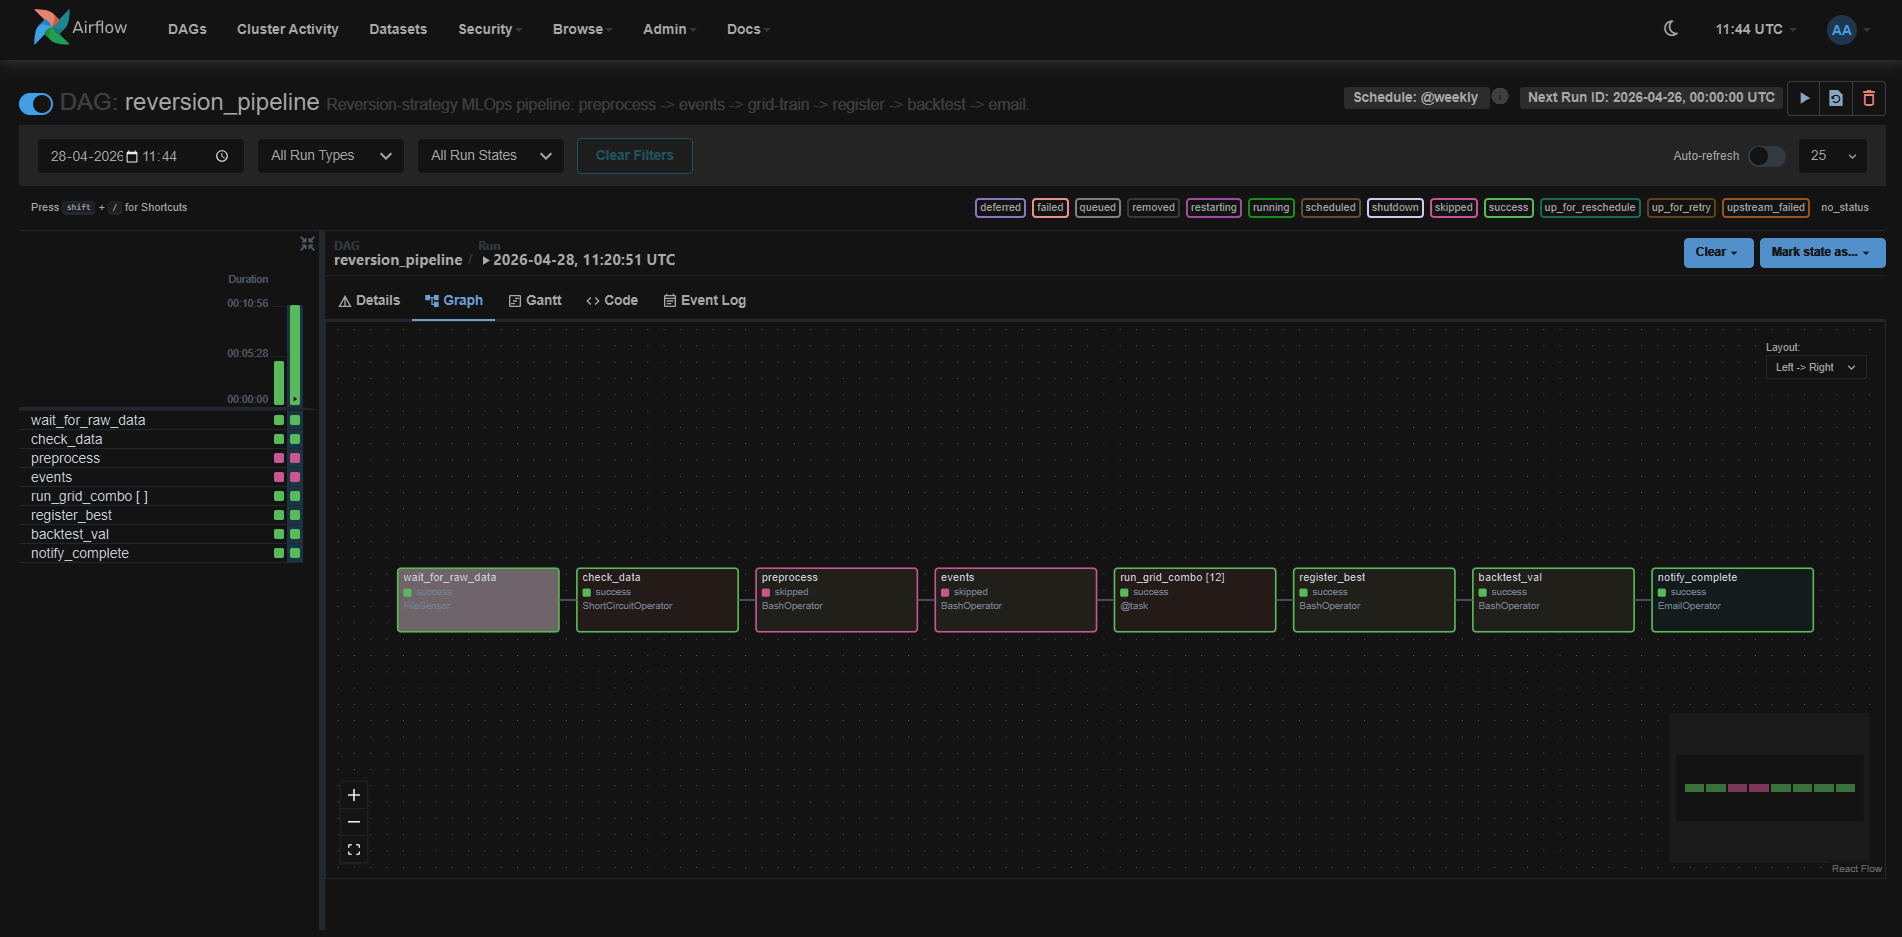
\includegraphics[width=0.95\linewidth]{images/airflow_pipeline_dag_run.png}
  \caption{\texttt{reversion\_pipeline} Graph view, mid-run. The dynamically-mapped \texttt{run\_grid\_combo} task expands to one node per (\emph{symbol}, \emph{position}, \emph{model\_type}, \emph{hp}) tuple; concurrency is capped at 2 by the \texttt{grid\_search} pool. Colour states distinguish queued / running / success / up\_for\_retry. Downstream: \texttt{register\_best} $\to$ \texttt{backtest\_val} $\to$ \texttt{notify\_complete}.}
  \label{fig:airflow-pipeline}
\end{figure}

\begin{figure}[h]
  \centering
  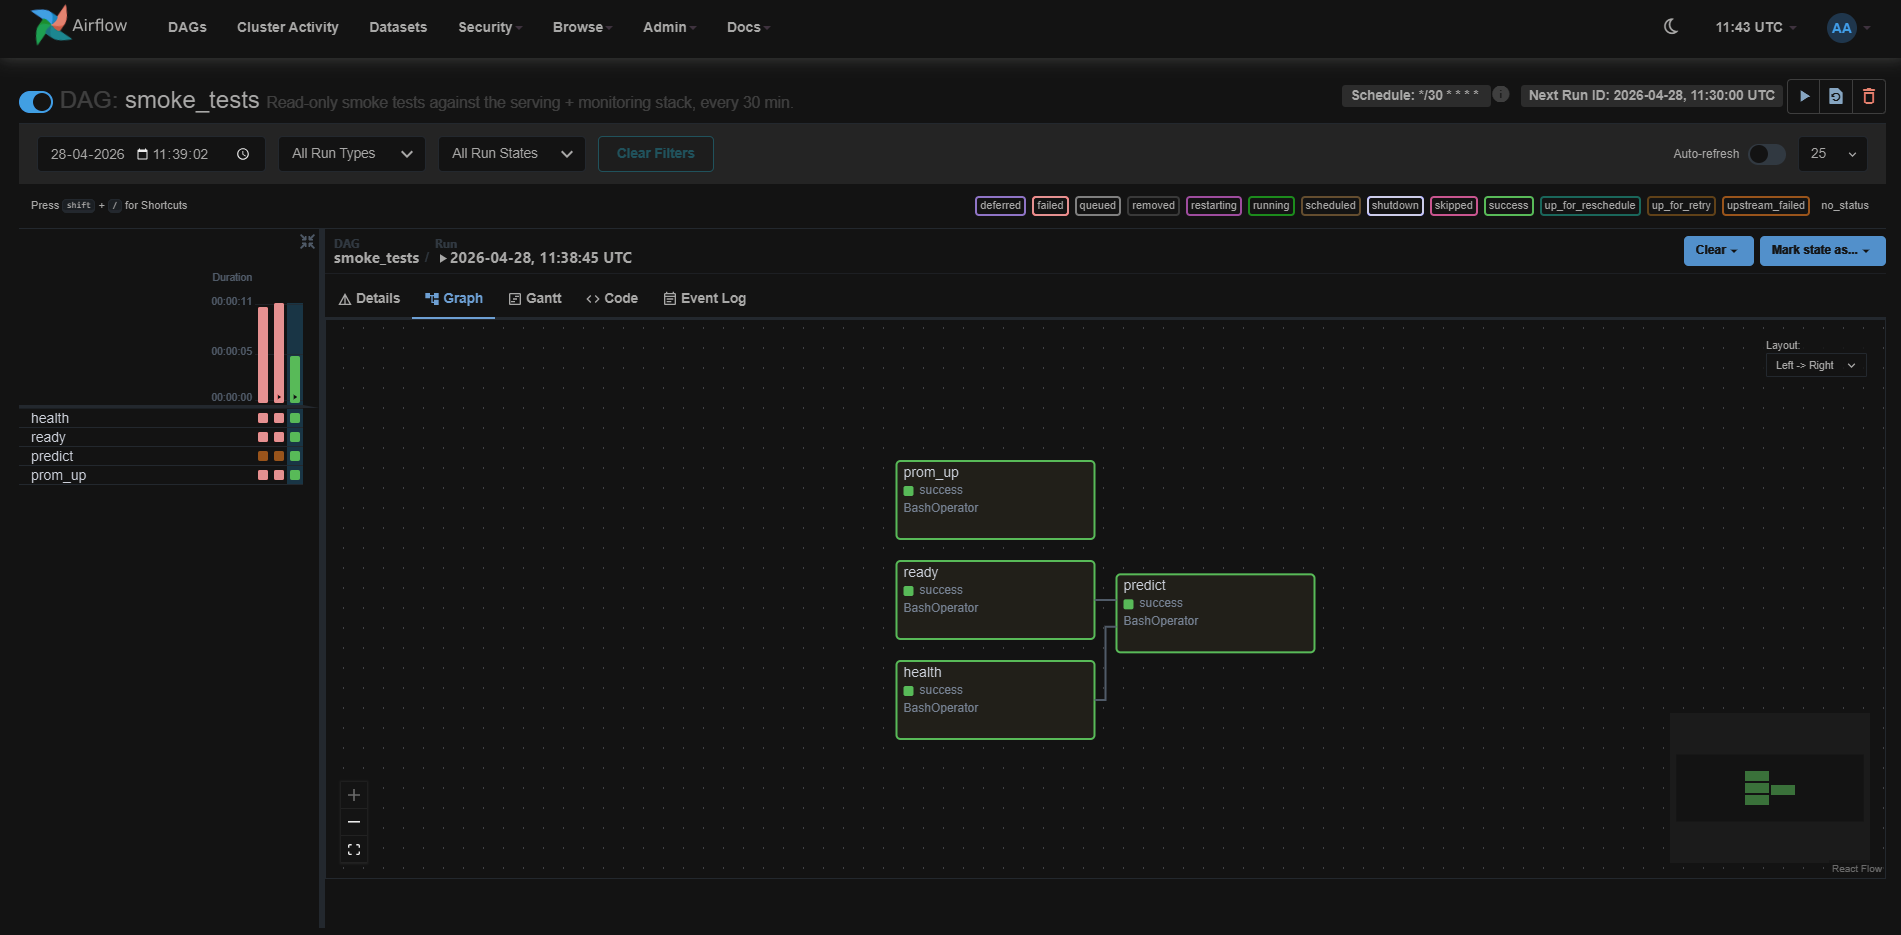
\includegraphics[width=0.95\linewidth]{images/airflow_smoke_test_dag_run.png}
  \caption{\texttt{smoke\_tests} Graph view --- separate DAG that exercises \texttt{health}, \texttt{ready}, \texttt{predict}, \texttt{prom-up} every 30 minutes. Independent of \texttt{reversion\_pipeline} so a stale serving container is detected within the smoke interval, not the weekly training cadence.}
  \label{fig:airflow-smoke}
\end{figure}

\begin{figure}[h]
  \centering
  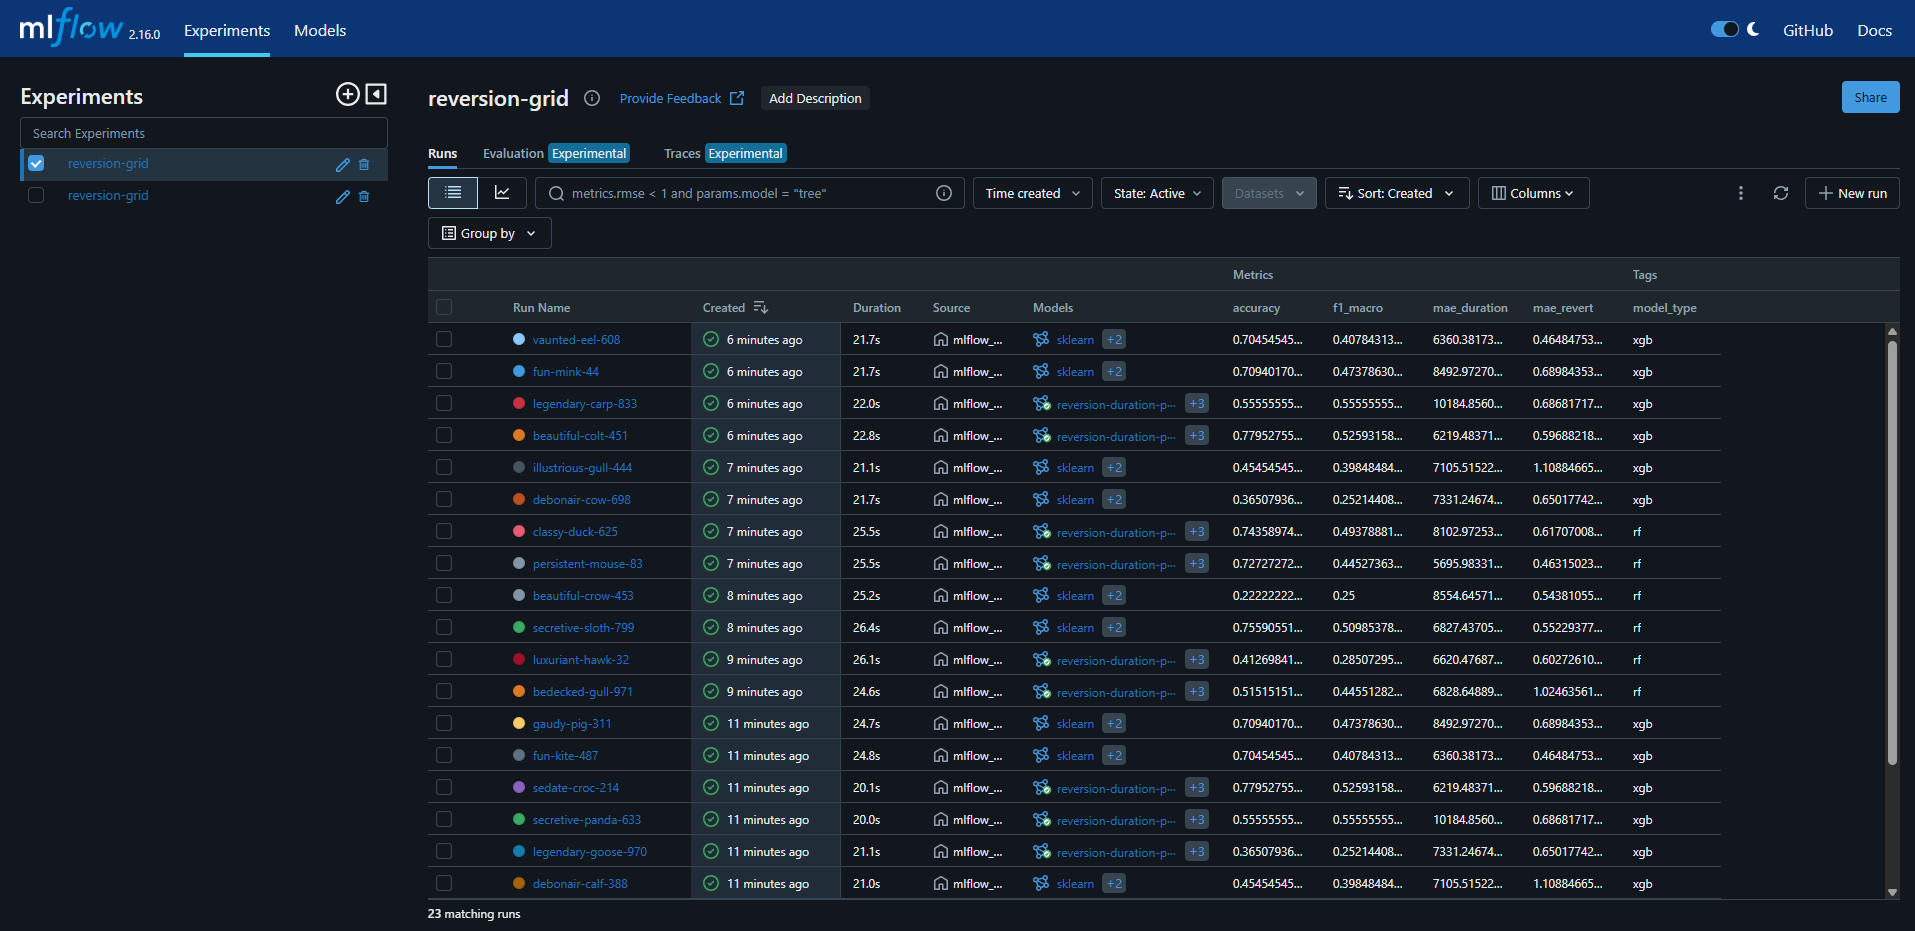
\includegraphics[width=0.95\linewidth]{images/mlflow_runs_list.png}
  \caption{MLflow runs in the \texttt{reversion-grid} experiment. Tags \texttt{symbol}, \texttt{position}, and \texttt{model\_type} are visible per row, which is what \texttt{scripts/register\_best.py} filters on when picking the per-(symbol, position) winner by \texttt{f1\_macro}.}
  \label{fig:mlflow-runs}
\end{figure}

\begin{figure}[h]
  \centering
  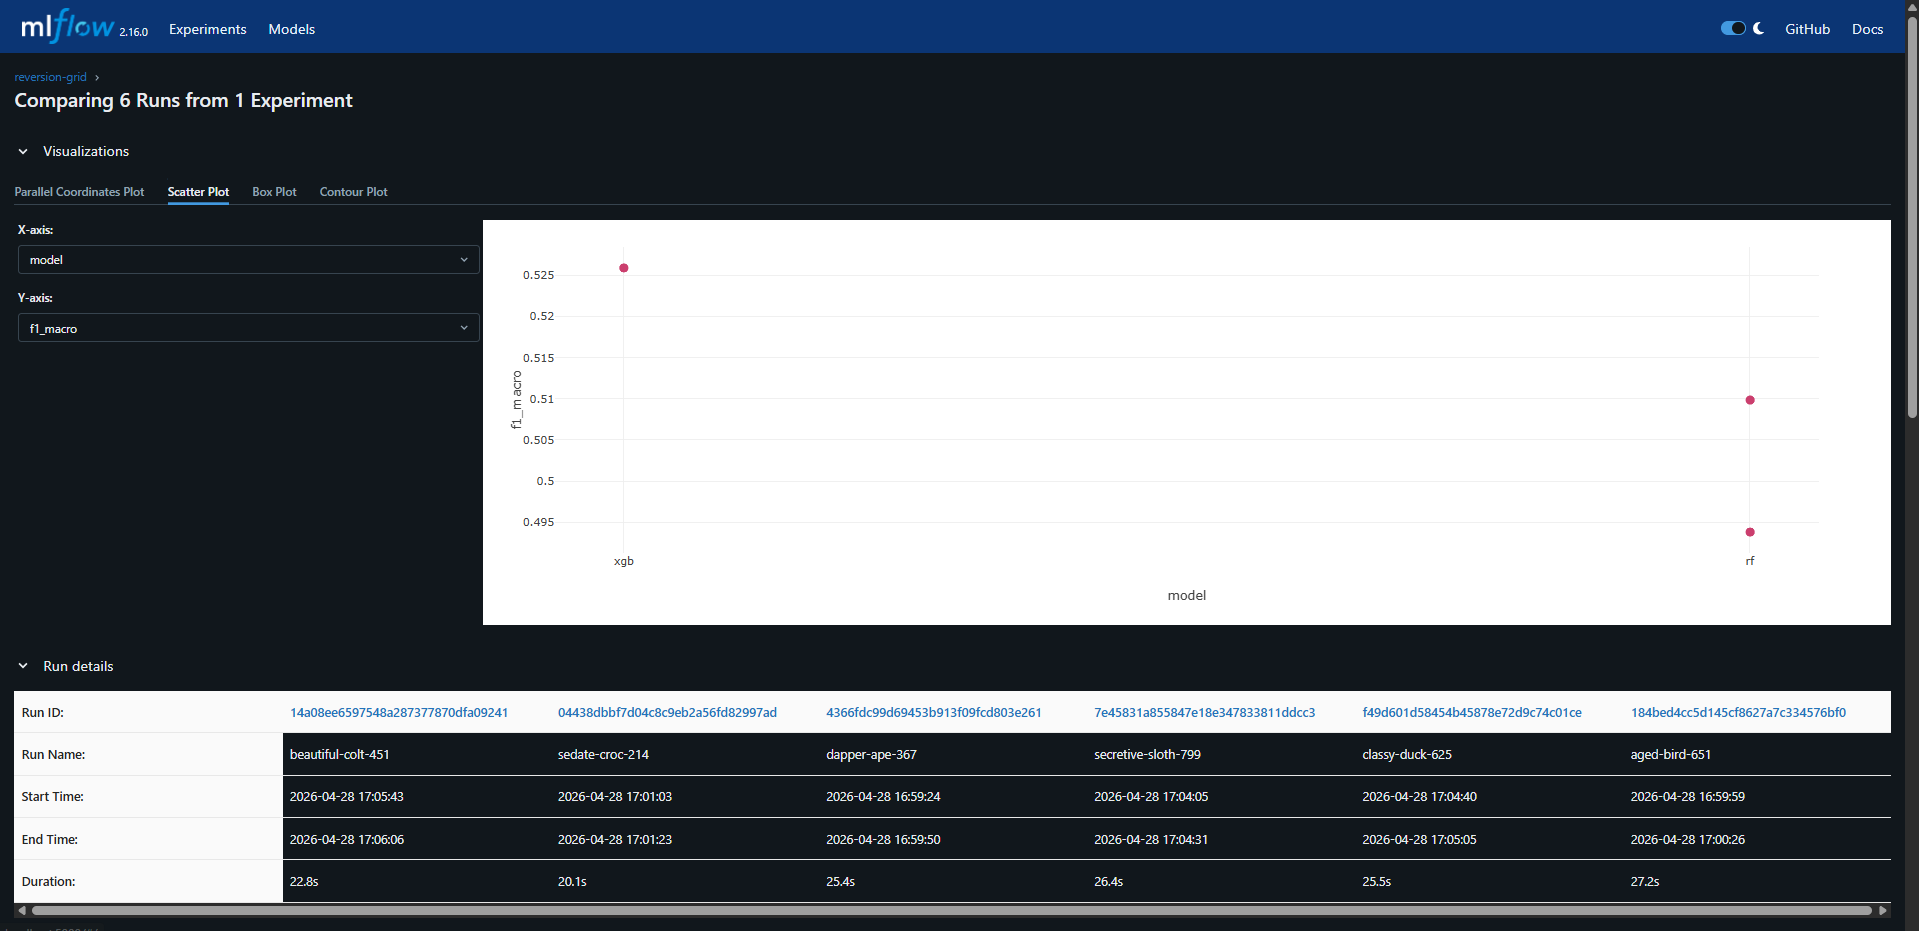
\includegraphics[width=0.95\linewidth]{images/mlflow_runs_comparison.png}
  \caption{MLflow run-comparison view across different model architectures (RF, XGB) and hyper-parameter combos. Side-by-side metrics (\texttt{f1\_macro}, \texttt{accuracy}, \texttt{mae\_duration}, \texttt{mae\_revert}) per run column let the operator see which (symbol, position, model\_type, hp) tuple wins the per-position selection.}
  \label{fig:mlflow-compare}
\end{figure}

\begin{figure}[h]
  \centering
  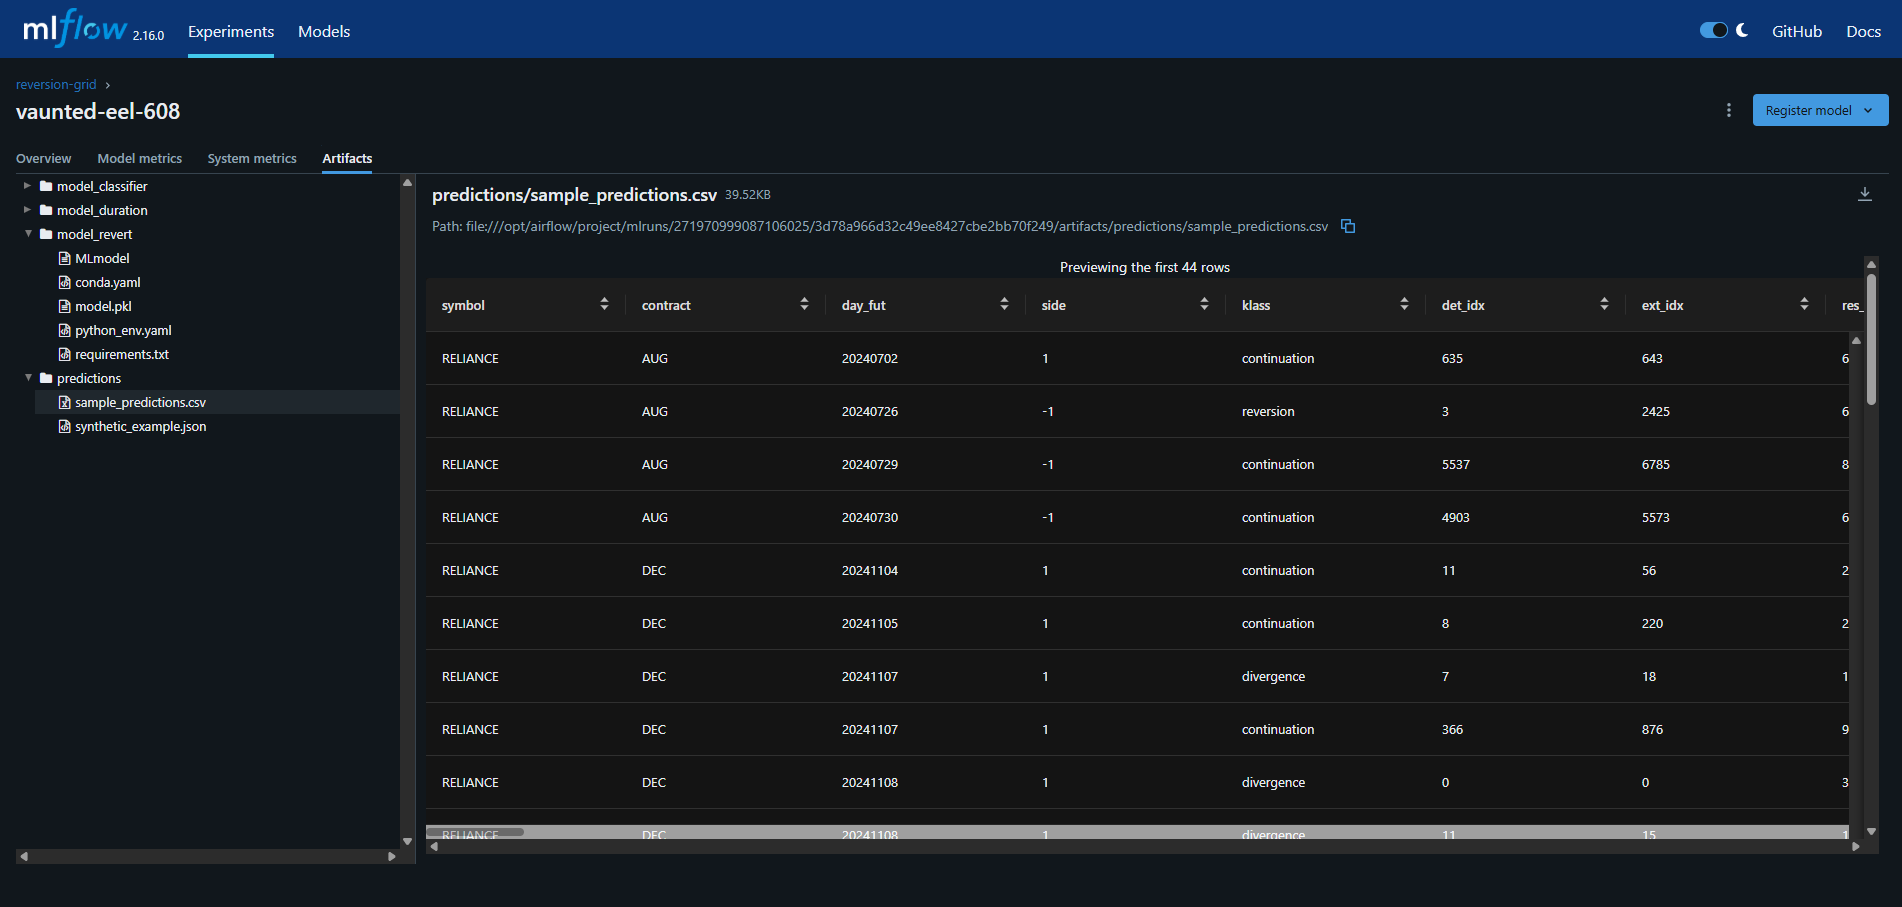
\includegraphics[width=0.95\linewidth]{images/mlflow_model_sample.png}
  \caption{Artefact view of one registered run, showing the three head models (\texttt{model\_classifier} / \texttt{model\_duration} / \texttt{model\_revert}) and the \texttt{predictions/} folder containing \texttt{sample\_predictions.csv} (200 paired (input, predicted, actual) rows) and \texttt{synthetic\_example.json} (deterministic feature row + all 3 head outputs). Both are written via \texttt{mlflow.log\_text} / \texttt{mlflow.log\_dict} --- no temp-file disk write.}
  \label{fig:mlflow-sample}
\end{figure}

\begin{figure}[h]
  \centering
  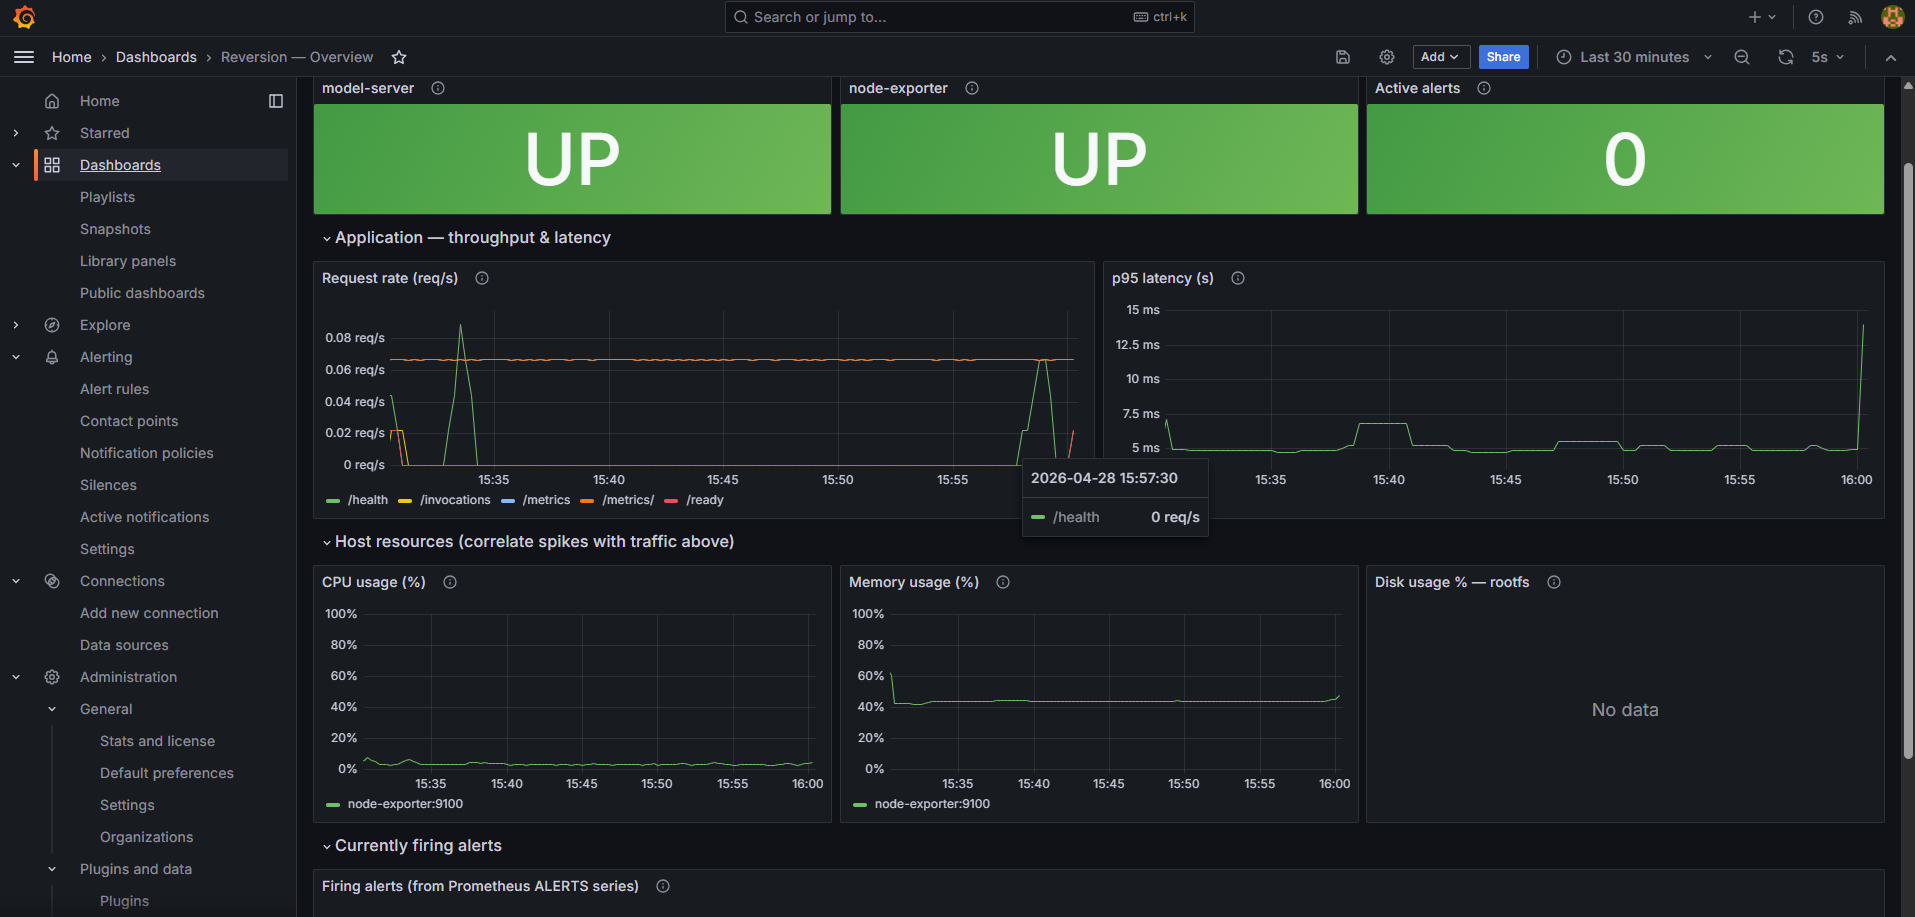
\includegraphics[width=0.95\linewidth]{images/grafana_reversion_overview.png}
  \caption{Grafana \texttt{Reversion --- Overview} dashboard: service-health stat panels at top, throughput + latency in the middle row, host CPU/memory/disk below. Single-pane view for ``is everything alive and serving traffic.''}
  \label{fig:grafana-overview}
\end{figure}

\begin{figure}[h]
  \centering
  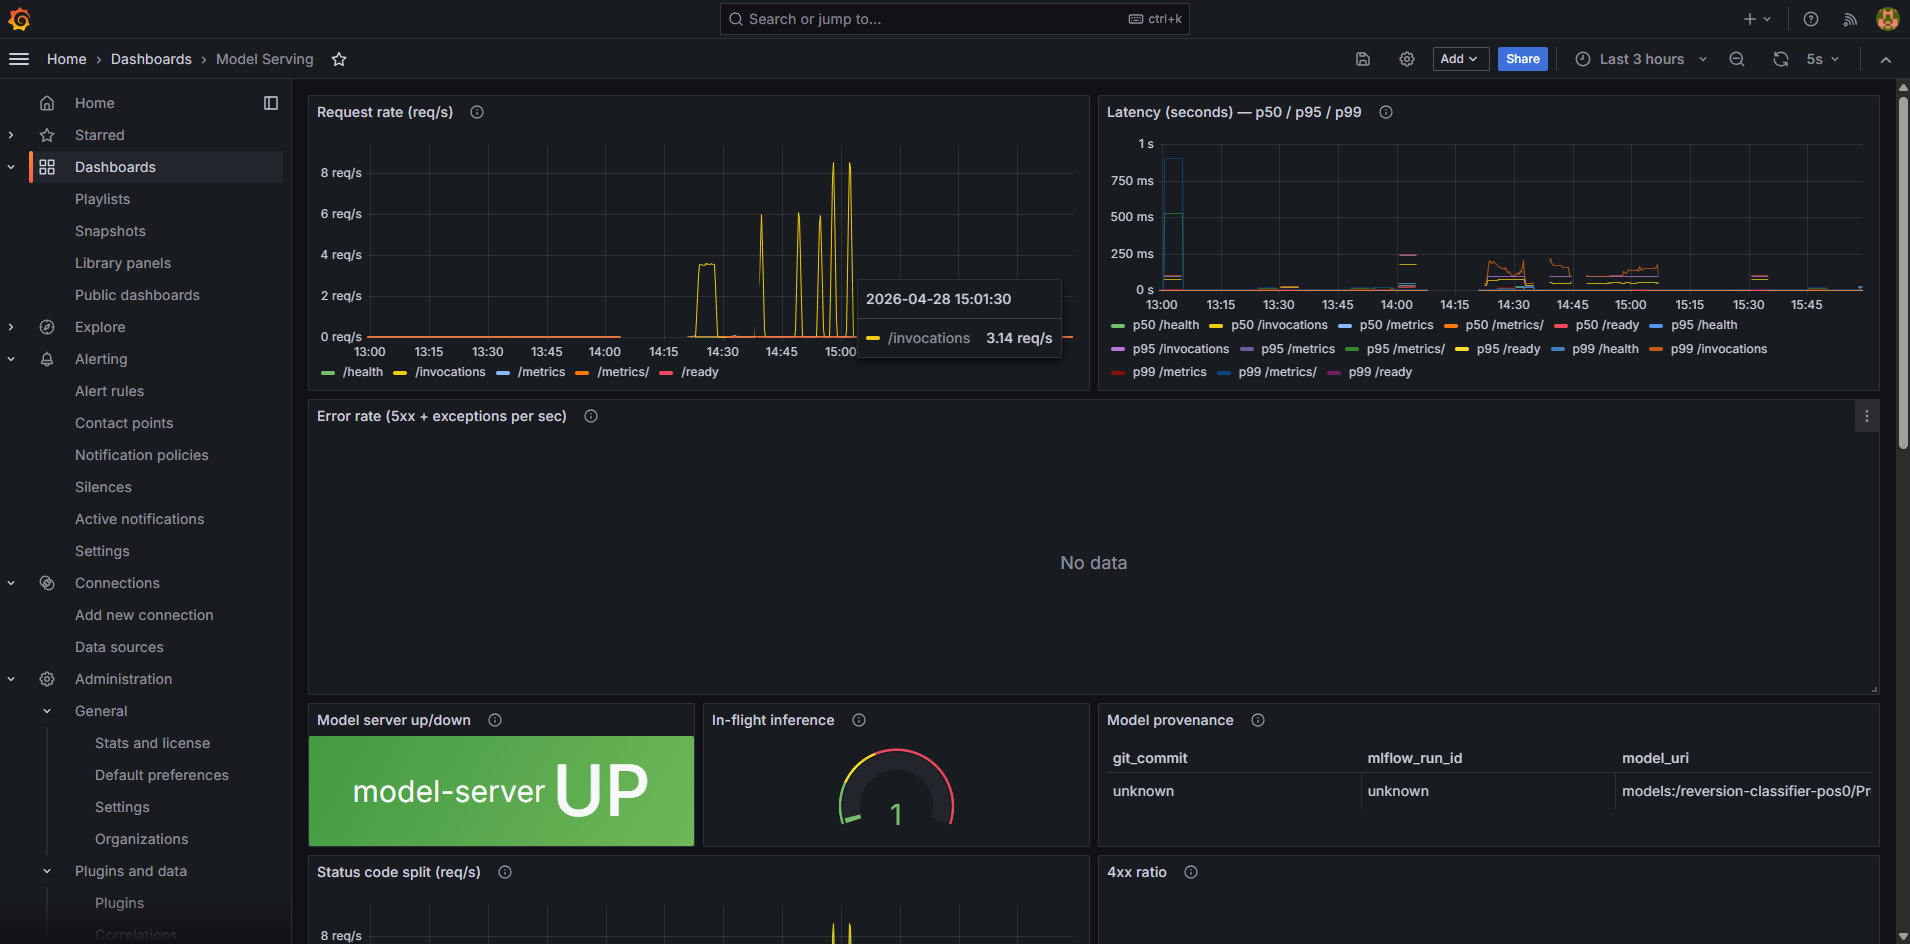
\includegraphics[width=0.95\linewidth]{images/grafana_serving_1.png}
  \caption{Grafana \texttt{Model Serving} dashboard, top half: request rate, latency quantiles (p50/p95/p99), error rate, server up/down, in-flight gauge, and the model-provenance table (\texttt{model\_uri}, \texttt{git\_commit}, \texttt{mlflow\_run\_id}).}
  \label{fig:grafana-serving-1}
\end{figure}

\begin{figure}[h]
  \centering
  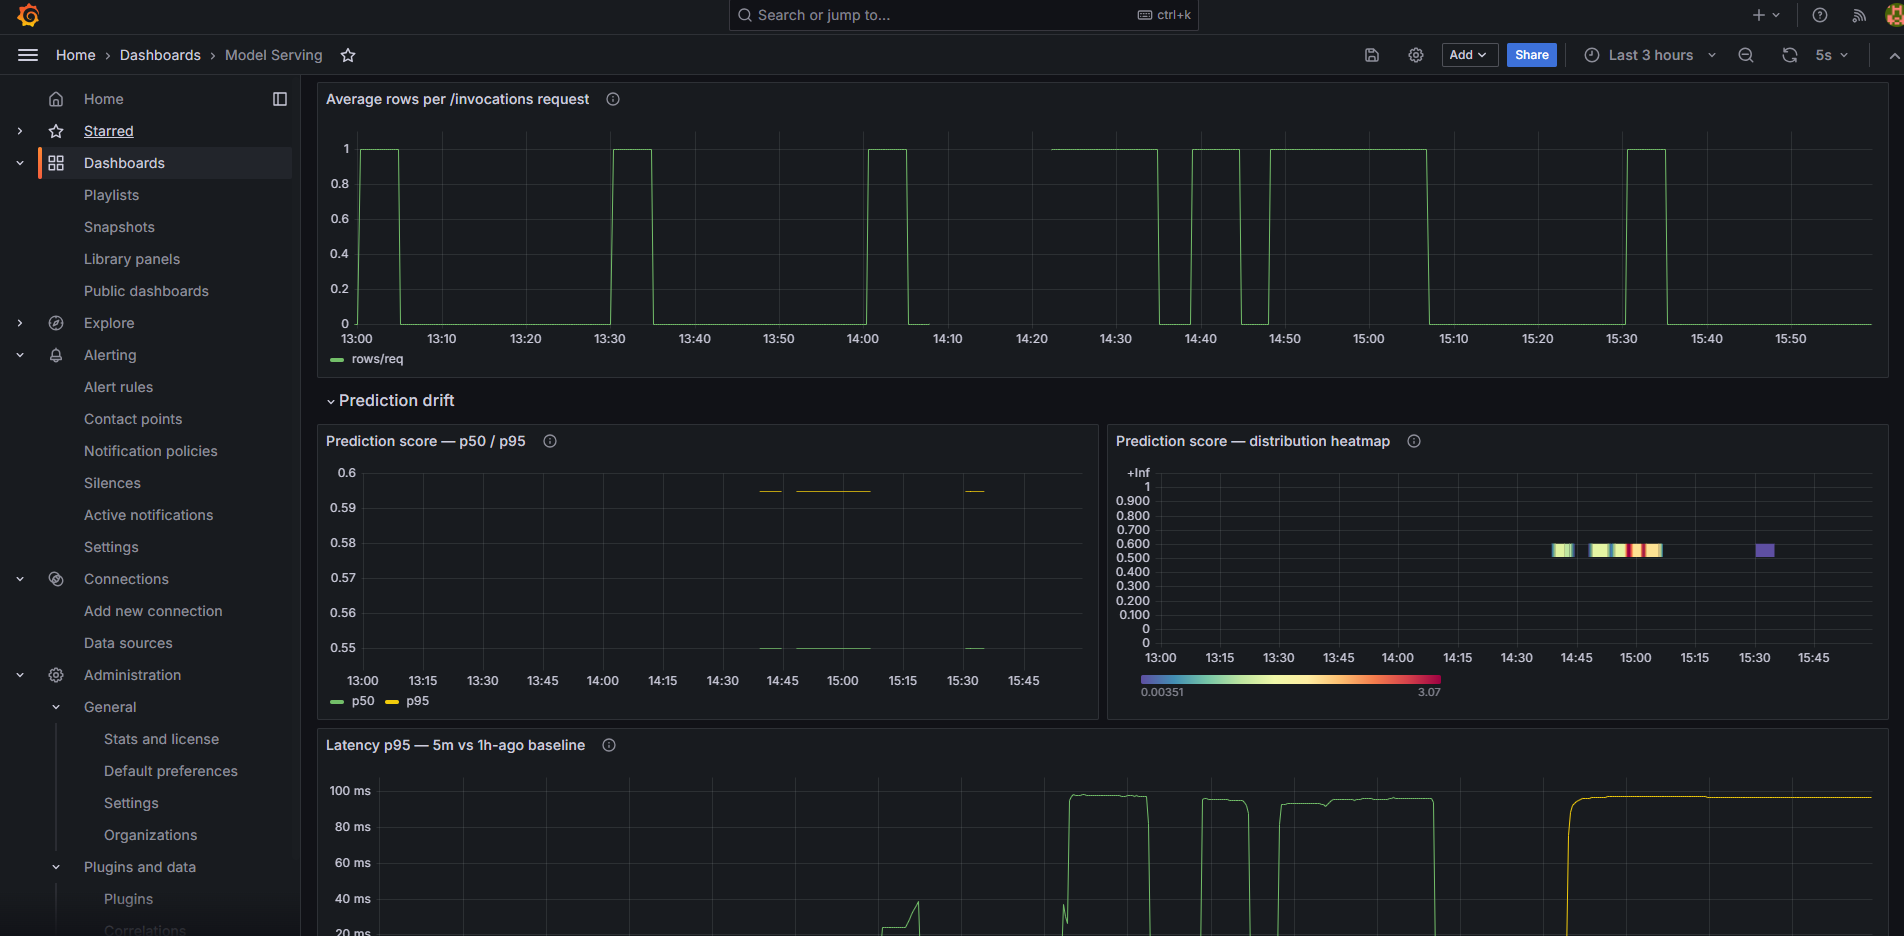
\includegraphics[width=0.95\linewidth]{images/grafan_serving_2.png}
  \caption{Same dashboard, bottom half: status-code split, 4xx ratio (schema-drift proxy), payload-rows mean, and the new \emph{Prediction drift} row --- prediction-score quantiles, distribution heatmap, and 5m-vs-1h-ago latency baseline. The score panels populate from \texttt{predict\_proba} max-class confidence (\texttt{src/serve.py:204--209}).}
  \label{fig:grafana-serving-2}
\end{figure}

\begin{figure}[h]
  \centering
  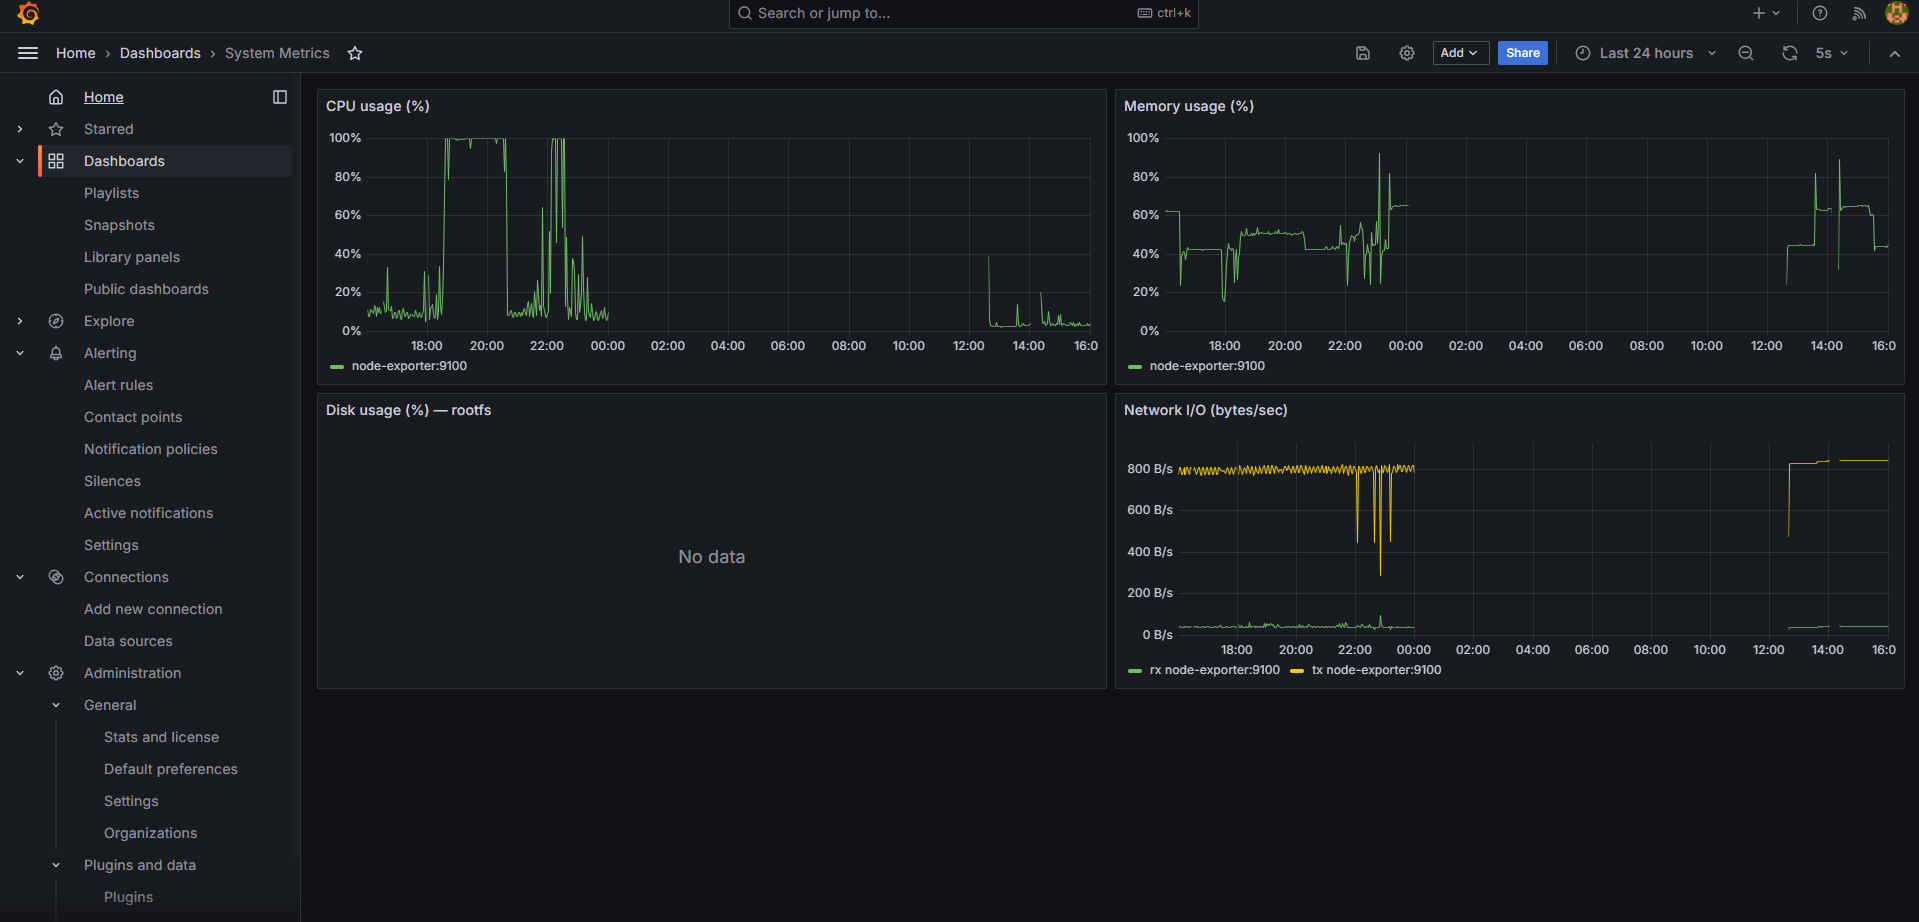
\includegraphics[width=0.95\linewidth]{images/grafana_system_metrics.png}
  \caption{Grafana \texttt{System Metrics} dashboard --- node-exporter scrape covering CPU\%, memory\%, rootfs disk\%, and network I/O. Used to correlate latency spikes on the serving dashboard with host saturation.}
  \label{fig:grafana-system}
\end{figure}

\begin{figure}[h]
  \centering
  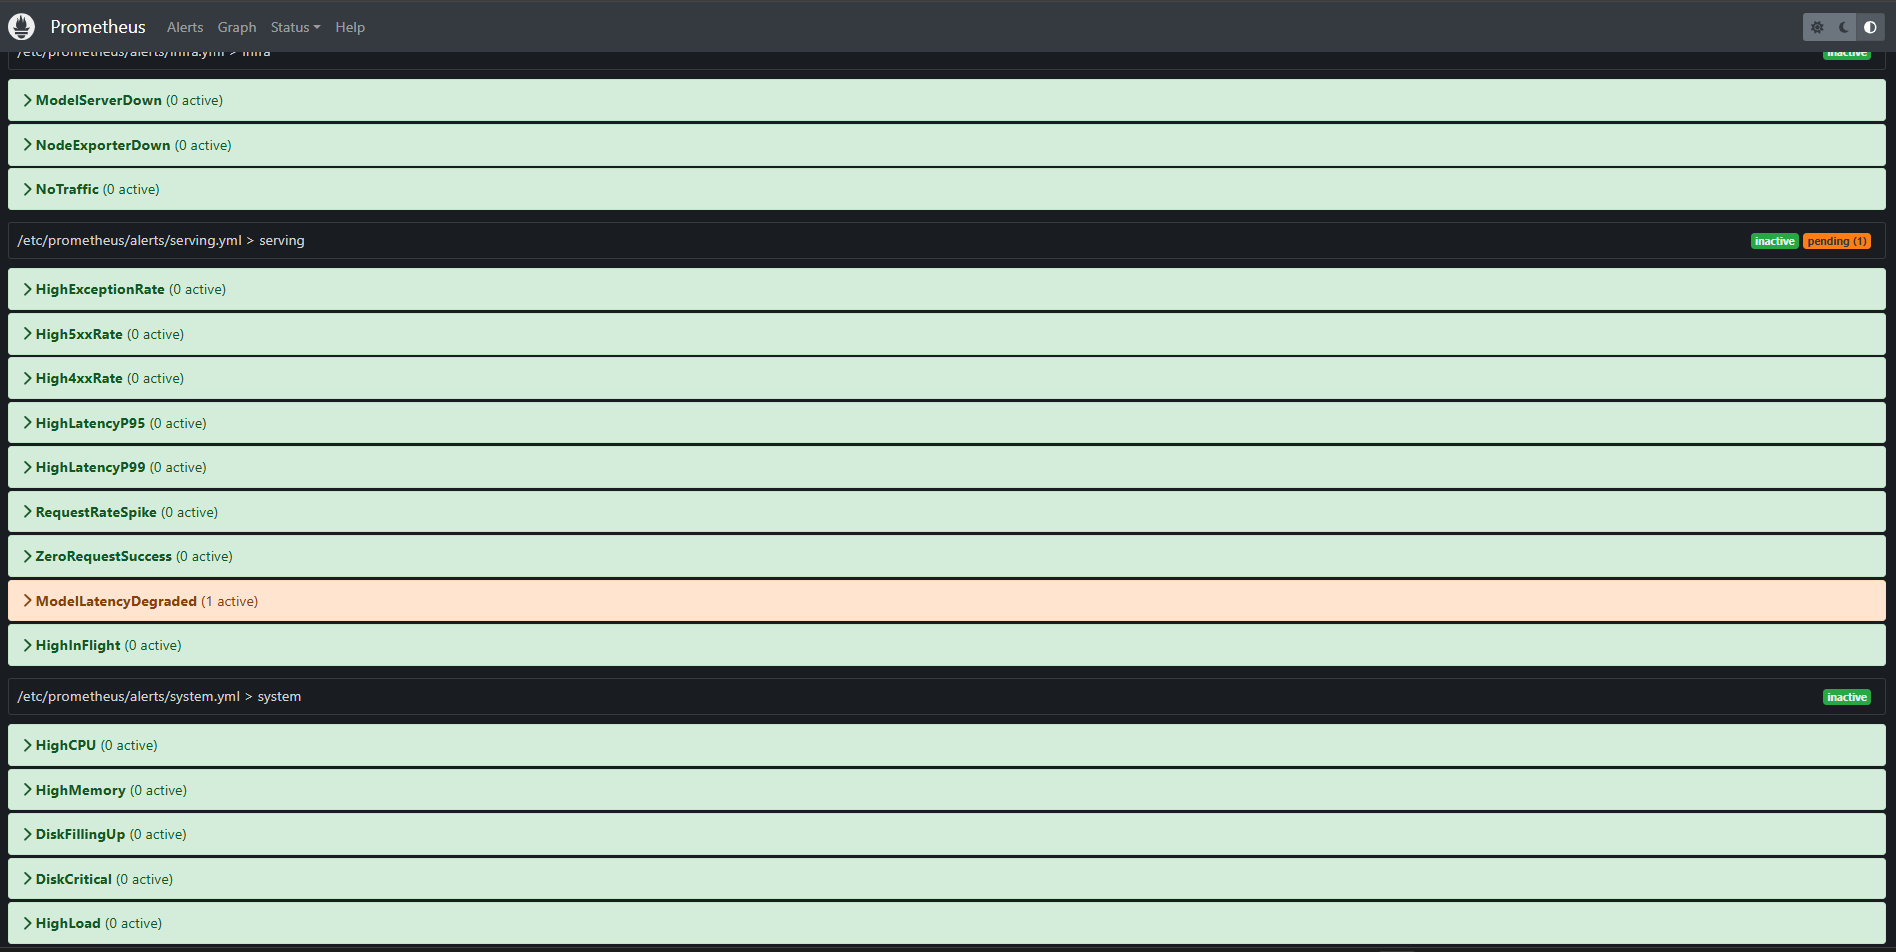
\includegraphics[width=0.8\linewidth]{images/prometheus_alerts_list.png}
  \caption{List of all alert rules registered with Prometheus, viewed at \texttt{:9090/alerts}. Three groups (\texttt{infra}, \texttt{serving}, \texttt{system}) defined under \texttt{monitoring/alerts/}; 17 rules total covering scrape health, latency degradation, error/exception rates, payload-schema drift, and host saturation.}
  \label{fig:prometheus-alerts-list}
\end{figure}

\begin{figure}[h]
  \centering
  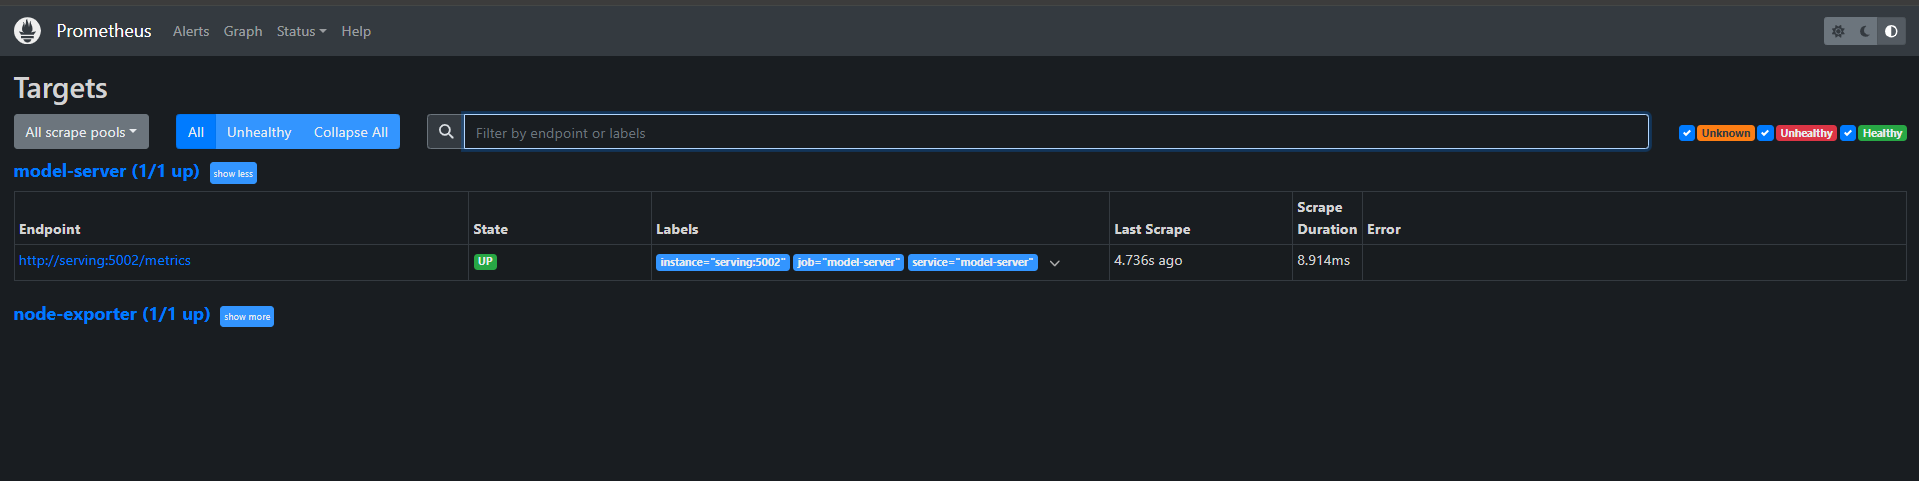
\includegraphics[width=0.8\linewidth]{images/prometheus_alerts.png}
  \caption{A firing Prometheus alert as viewed through the UI at port 9090. \texttt{Active} state is reached after the rule's \texttt{for:} window elapses; Alertmanager then routes by severity.}
  \label{fig:prometheus-alert}
\end{figure}

\begin{figure}[h]
  \centering
  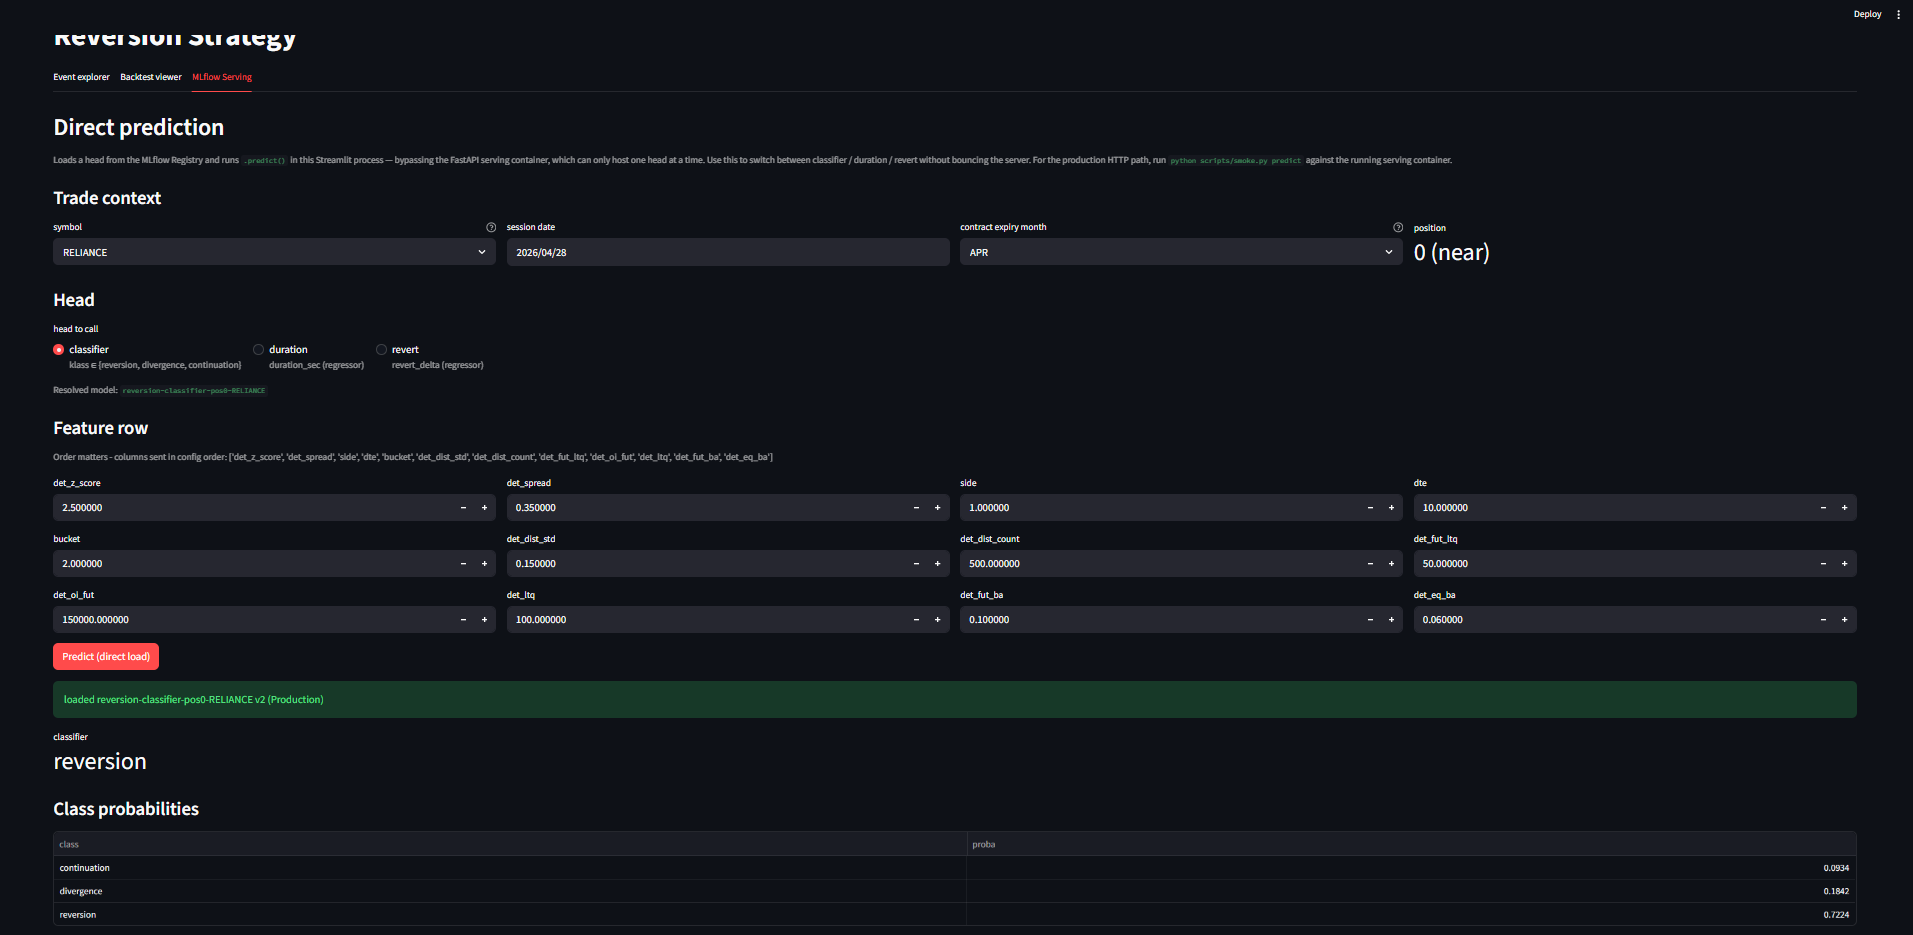
\includegraphics[width=0.95\linewidth]{images/streamlit_ui_reliance_pred.png}
  \caption{Streamlit tab~3, \emph{Direct prediction}. Trade-context inputs (\emph{symbol} = RELIANCE, session date, contract expiry month) derive the position automatically; the head selector picks classifier / duration / revert; the resolved model name (\texttt{reversion-classifier-posX-RELIANCE}) is shown above the feature inputs. Loading uses \texttt{mlflow.sklearn.load\_model("runs:/...")} in-process --- the FastAPI server is not on the path.}
  \label{fig:streamlit-pred}
\end{figure}

\begin{figure}[h]
  \centering
  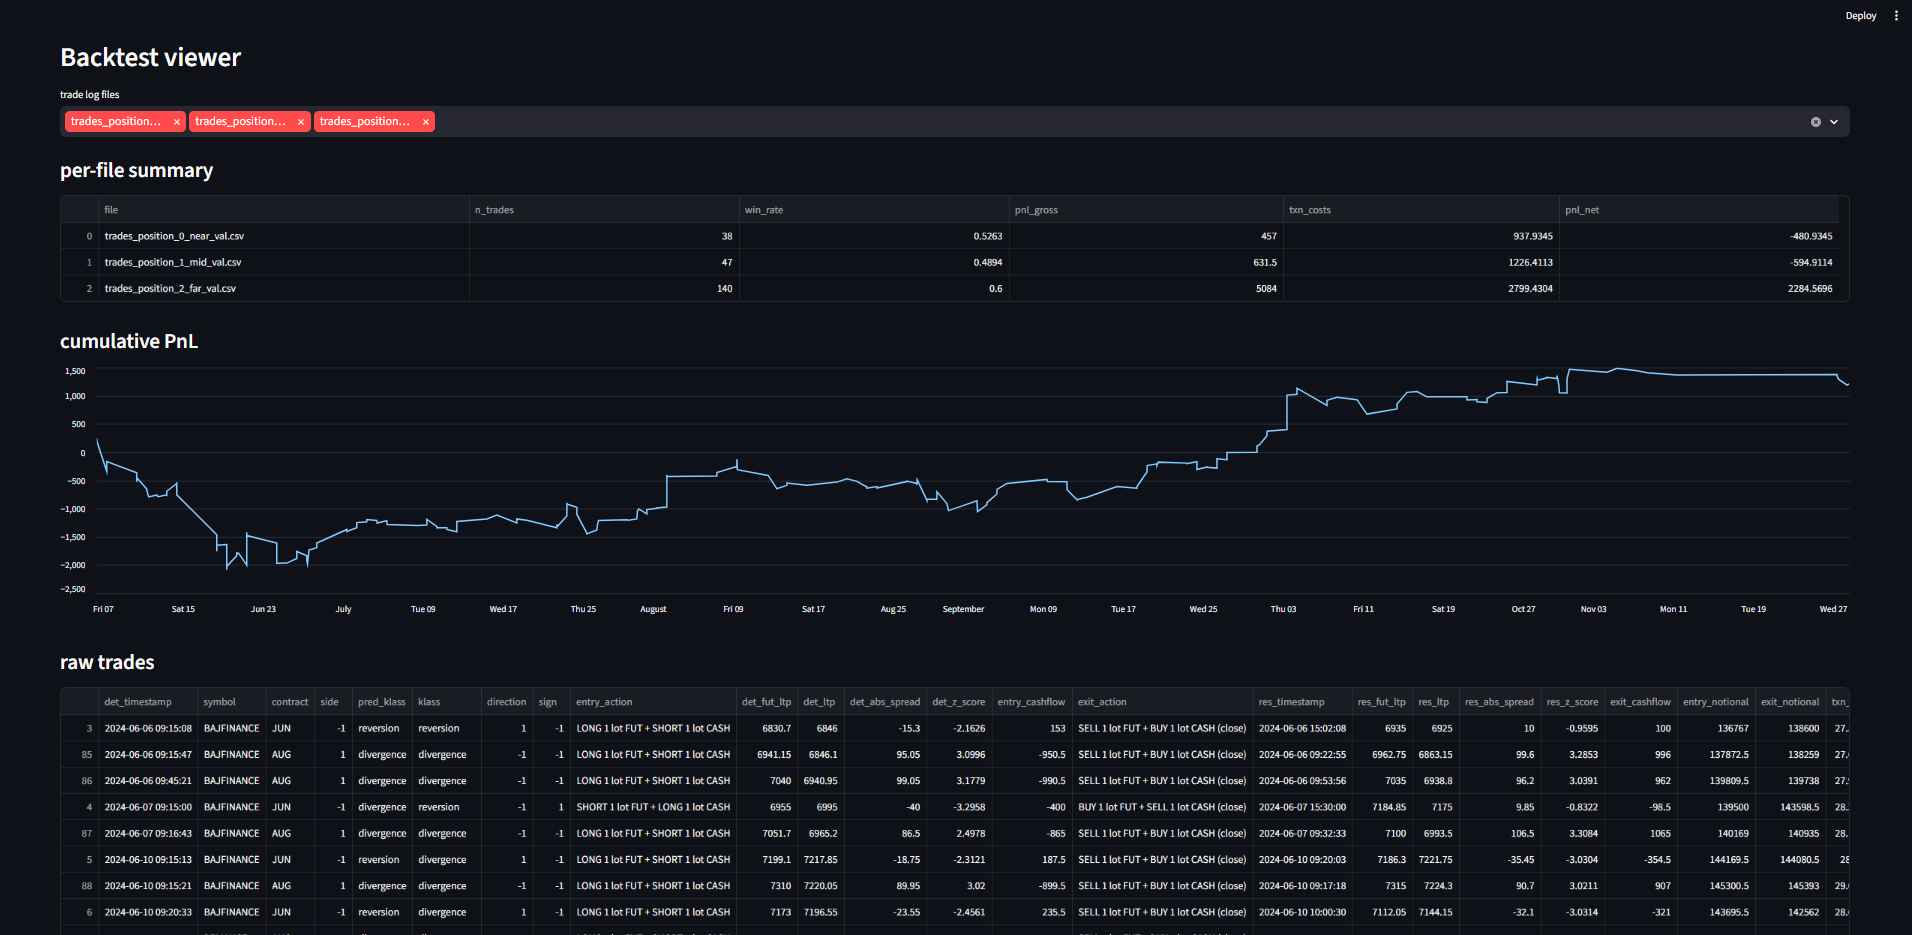
\includegraphics[width=0.95\linewidth]{images/streamlit_backtest_viewer.png}
  \caption{Streamlit tab~2, \emph{Backtest viewer}. Multi-selecting per-(symbol, position) trade logs renders the per-file PnL summary (n\_trades, win\_rate, gross/net), the cumulative-equity line, and the raw trades table.}
  \label{fig:streamlit-backtest}
\end{figure}

\begin{figure}[h]
  \centering
  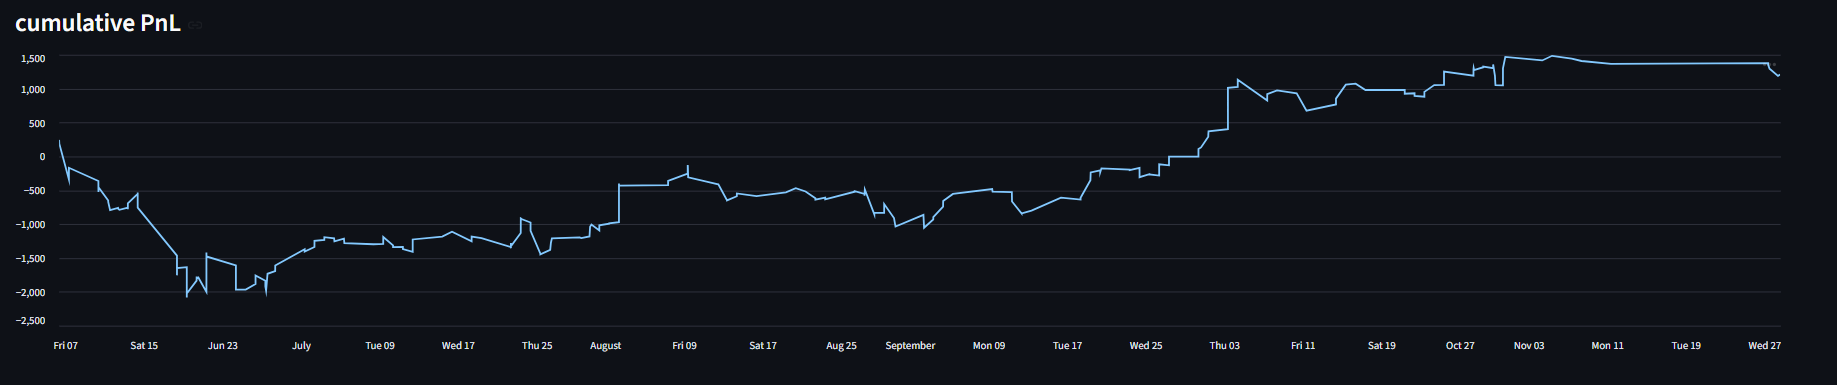
\includegraphics[width=0.8\linewidth]{images/backtest_graph.png}
  \caption{Backtest equity curve over the val window (Jul--Dec 2024). Cumulative PnL aggregated across all (symbol, position) trade logs from the same registry promotion; produced by \texttt{python src/backtest.py --split val} and rendered through Streamlit tab~2.}
  \label{fig:backtest-equity}
\end{figure}

\begin{figure}[h]
  \centering
  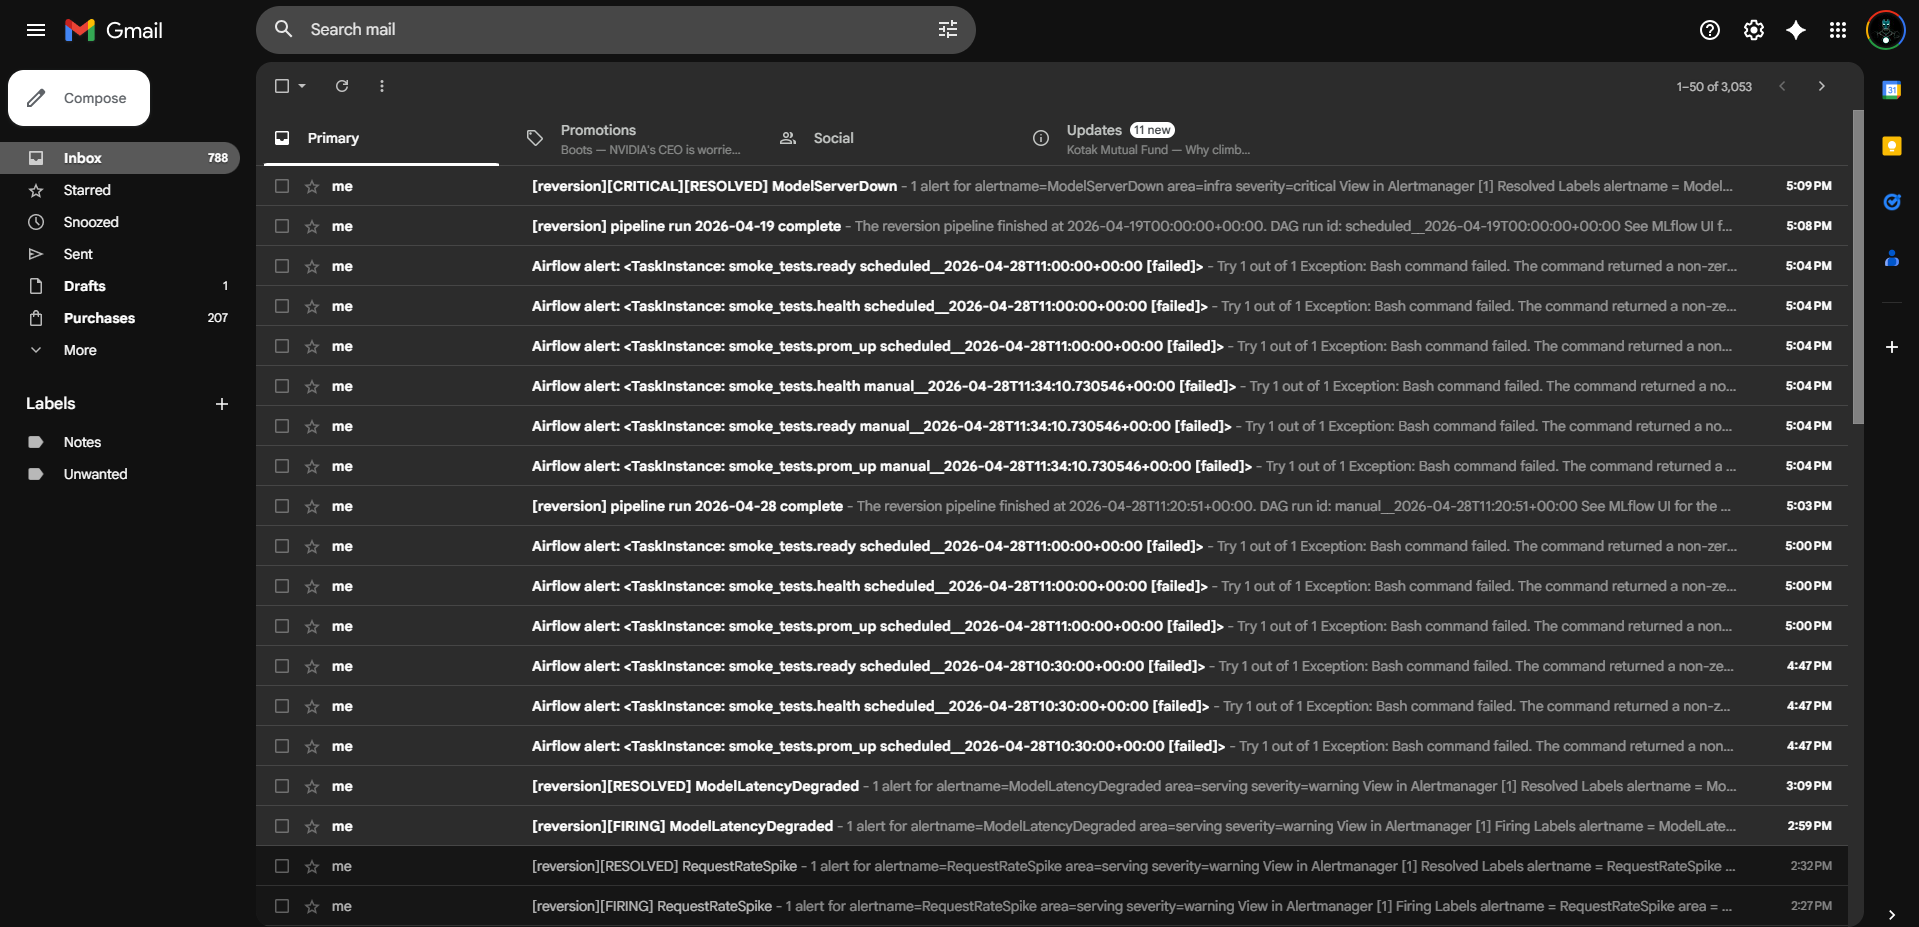
\includegraphics[width=0.8\linewidth]{images/email_alerts_overview.png}
  \caption{Gmail inbox showing alerts delivered through the Alertmanager $\to$ SMTP path (\texttt{HighExceptionRate}, \texttt{High4xxRate}, etc.). Generated with \texttt{python scripts/smoke.py fire-alerts --mode all}.}
  \label{fig:email-alerts}
\end{figure}

\end{document}
